% =============================================================================
%  এমএসসি প্রকল্প প্রতিবেদন — বাংলা সংস্করণ
%  (Bangla version of main.tex; the English report is unchanged)
%
%  Compile with XeLaTeX (Unicode Bengali needs it):
%     tectonic -X compile main_bn.tex           (this PC: ../.tex/Library/bin/tectonic.exe)
%  or on Overleaf: Menu -> Compiler = XeLaTeX, Main document = main_bn.tex
%  Font: "Nirmala UI" (Windows) if present, otherwise "FreeSerif" (in every TeX Live / Overleaf).
%  Numbers come from generated/numbers.tex; tables from tables_bn/ (both generated by the pipeline).
% =============================================================================
\documentclass[12pt,a4paper,oneside]{report}

% ---------------------------------------------------------------- Bengali fonts (XeLaTeX)
\usepackage{fontspec}
\IfFontExistsTF{Nirmala UI}
  {\setmainfont{Nirmala UI}[Script=Bengali, AutoFakeSlant=0.18]
   \setsansfont{Nirmala UI}[Script=Bengali, AutoFakeSlant=0.18]}
  {\setmainfont{FreeSerif}[Script=Bengali]
   \setsansfont{FreeSans}[Script=Bengali]}

% ---------------------------------------------------------------- packages (same as the English report)
\usepackage[margin=2.5cm,left=3cm]{geometry}
\usepackage{setspace}\setstretch{1.45}
\usepackage{graphicx}
\usepackage{booktabs,tabularx,longtable,array,multirow}
\usepackage{amsmath,amssymb}
\usepackage{xcolor}
\usepackage{caption}\captionsetup{font=small,labelfont=bf,skip=6pt}
\usepackage{float}
\usepackage{adjustbox}
\usepackage{enumitem}
\usepackage{xspace}
\usepackage{listings}
\usepackage{tikz}\usetikzlibrary{arrows.meta,positioning,shapes.geometric,shapes.multipart,fit,backgrounds}
\usepackage{fancyhdr}
\usepackage{titlesec}
\usepackage[round,authoryear]{natbib}
\usepackage[hidelinks]{hyperref}
\usepackage[nameinlink,capitalise]{cleveref}

\definecolor{brand}{HTML}{1F4E79}
\definecolor{accent}{HTML}{C55A11}
\definecolor{codebg}{HTML}{F5F7FA}
\titleformat{\chapter}[display]{\normalfont\huge\bfseries\color{brand}}{\chaptertitlename\ \thechapter}{12pt}{\Huge}
\titlespacing*{\chapter}{0pt}{-10pt}{24pt}
\titleformat{\section}{\normalfont\Large\bfseries\color{brand}}{\thesection}{1em}{}
\titleformat{\subsection}{\normalfont\large\bfseries}{\thesubsection}{1em}{}
\setlength{\headheight}{15pt}
\pagestyle{fancy}\fancyhf{}\fancyhead[L]{\small\nouppercase{\leftmark}}\fancyfoot[C]{\thepage}
\renewcommand{\headrulewidth}{0.4pt}
\fancypagestyle{plain}{\fancyhf{}\fancyfoot[C]{\thepage}\renewcommand{\headrulewidth}{0pt}}
\lstset{basicstyle=\ttfamily\footnotesize,backgroundcolor=\color{codebg},frame=single,rulecolor=\color{gray!40},
  breaklines=true,columns=fullflexible,keywordstyle=\color{brand}\bfseries,commentstyle=\color{gray},
  stringstyle=\color{accent},showstringspaces=false,xleftmargin=4pt,framexleftmargin=4pt}
\setlist{itemsep=2pt,topsep=4pt}
\graphicspath{{figures/}}
\setlength{\emergencystretch}{3em}

% ---------------------------------------------------------------- Bangla names for document parts
\renewcommand{\contentsname}{সূচিপত্র}
\renewcommand{\listfigurename}{চিত্রের তালিকা}
\renewcommand{\listtablename}{সারণির তালিকা}
\renewcommand{\bibname}{তথ্যসূত্র}
\renewcommand{\chaptername}{অধ্যায়}
\renewcommand{\appendixname}{পরিশিষ্ট}
\renewcommand{\figurename}{চিত্র}
\renewcommand{\tablename}{সারণি}
\crefname{chapter}{অধ্যায়}{অধ্যায়}\Crefname{chapter}{অধ্যায়}{অধ্যায়}
\crefname{appendix}{পরিশিষ্ট}{পরিশিষ্ট}\Crefname{appendix}{পরিশিষ্ট}{পরিশিষ্ট}
\crefname{section}{অনুচ্ছেদ}{অনুচ্ছেদ}\Crefname{section}{অনুচ্ছেদ}{অনুচ্ছেদ}
\crefname{subsection}{অনুচ্ছেদ}{অনুচ্ছেদ}\Crefname{subsection}{অনুচ্ছেদ}{অনুচ্ছেদ}
\crefname{figure}{চিত্র}{চিত্র}\Crefname{figure}{চিত্র}{চিত্র}
\crefname{table}{সারণি}{সারণি}\Crefname{table}{সারণি}{সারণি}
\crefname{equation}{সমীকরণ}{সমীকরণ}\Crefname{equation}{সমীকরণ}{সমীকরণ}

% ---------------------------------------------------------------- generated results
% AUTO-GENERATED by src/dancake/export.py - do not edit by hand; re-run the pipeline instead.
\newcommand{\NRows}{500,000\xspace}
\newcommand{\NCols}{23\xspace}
\newcommand{\NProducts}{52\xspace}
\newcommand{\NRegions}{11\xspace}
\newcommand{\NChannels}{4\xspace}
\newcommand{\NCustTypes}{5\xspace}
\newcommand{\DateMin}{January 2020\xspace}
\newcommand{\DateMax}{September 2026\xspace}
\newcommand{\NOutlierFlags}{1,334\xspace}
\newcommand{\OutlierPct}{0.27\xspace}
\newcommand{\WarehouseSeconds}{3.5\xspace}
\newcommand{\TotalSales}{318.4\xspace}
\newcommand{\TotalUnits}{3.09\xspace}
\newcommand{\AOV}{637\xspace}
\newcommand{\AvgDiscount}{2.35\xspace}
\newcommand{\DiscountCost}{7.67\xspace}
\newcommand{\CAGRSales}{16.6\xspace}
\newcommand{\CAGRUnits}{5.0\xspace}
\newcommand{\CAGRPrice}{11.2\xspace}
\newcommand{\AvgVolGrowth}{5.0\xspace}
\newcommand{\AvgPriceGrowth}{11.3\xspace}
\newcommand{\YTDGrowth}{14.0\xspace}
\newcommand{\PeakMonth}{December\xspace}
\newcommand{\PeakIndex}{124.8\xspace}
\newcommand{\TroughMonth}{February\xspace}
\newcommand{\TroughIndex}{85.7\xspace}
\newcommand{\DecPerDay}{122.6\xspace}
\newcommand{\FebPerDay}{92.1\xspace}
\newcommand{\NovIndex}{106.5\xspace}
\newcommand{\OctIndex}{104.1\xspace}
\newcommand{\KWMonthH}{510.9\xspace}
\newcommand{\DowCV}{0.62\xspace}
\newcommand{\TopCategory}{Muffin\xspace}
\newcommand{\TopCategoryShare}{22.4\xspace}
\newcommand{\TopTenShare}{38.5\xspace}
\newcommand{\NClassA}{27\xspace}
\newcommand{\NClassB}{12\xspace}
\newcommand{\NClassC}{13\xspace}
\newcommand{\DhakaShare}{43.9\xspace}
\newcommand{\DhakaCtgShare}{58.3\xspace}
\newcommand{\GTShare}{45.6\xspace}
\newcommand{\MTShare}{25.6\xspace}
\newcommand{\DistShare}{22.9\xspace}
\newcommand{\EcomShare}{5.9\xspace}
\newcommand{\DistQty}{11.4\xspace}
\newcommand{\EcomQty}{3.7\xspace}
\newcommand{\GTQty}{5.3\xspace}
\newcommand{\MTQty}{6.3\xspace}
\newcommand{\LargeRate}{19.2\xspace}
\newcommand{\QtySkew}{3.12\xspace}
\newcommand{\ValueSkew}{4.47\xspace}
\newcommand{\QtyMedian}{4\xspace}
\newcommand{\EpsChannel}{0.087\xspace}
\newcommand{\EpsRegion}{0.055\xspace}
\newcommand{\PCustType}{0.62\xspace}
\newcommand{\RhoDisc}{0.0010\xspace}
\newcommand{\PDisc}{0.48\xspace}
\newcommand{\CramerV}{0.252\xspace}
\newcommand{\CorrSalesQty}{0.70\xspace}
\newcommand{\CorrSalesPrice}{0.68\xspace}
\newcommand{\CorrQtyPrice}{0.025\xspace}
\newcommand{\Elasticity}{0.09\xspace}
\newcommand{\ElasticityLo}{-0.28\xspace}
\newcommand{\ElasticityHi}{0.46\xspace}
\newcommand{\ElasticityP}{0.62\xspace}
\newcommand{\ElasticityNaive}{0.42\xspace}
\newcommand{\ElasticityRtwo}{0.81\xspace}
\newcommand{\FastCategory}{Layer Cake\xspace}
\newcommand{\FastCategoryCAGR}{67.7\xspace}
\newcommand{\PanelSeries}{52\xspace}
\newcommand{\PanelTrain}{2,912\xspace}
\newcommand{\PanelTest}{1,092\xspace}
\newcommand{\PanelFeatures}{24\xspace}
\newcommand{\TestMonths}{21\xspace}
\newcommand{\BestReg}{Support Vector Regression\xspace}
\newcommand{\BestRegRMSE}{115.2\xspace}
\newcommand{\BestRegMAE}{90.6\xspace}
\newcommand{\BestRegWAPE}{11.13\xspace}
\newcommand{\BestRegRtwo}{0.744\xspace}
\newcommand{\BestRegMAPE}{12.26\xspace}
\newcommand{\SNaiveRMSE}{152.4\xspace}
\newcommand{\SNaiveWAPE}{14.74\xspace}
\newcommand{\SNaiveRtwo}{0.551\xspace}
\newcommand{\NaiveRMSE}{176.2\xspace}
\newcommand{\GainVsSNaive}{24.4\xspace}
\newcommand{\GainVsNaive}{34.6\xspace}
\newcommand{\LinRMSE}{117.7\xspace}
\newcommand{\RFRMSE}{120.1\xspace}
\newcommand{\XGBRMSE}{119.6\xspace}
\newcommand{\DTRMSE}{134.1\xspace}
\newcommand{\GBRMSE}{122.9\xspace}
\newcommand{\KNNRMSE}{126.0\xspace}
\newcommand{\SVRRMSE}{115.2\xspace}
\newcommand{\WorstRegRMSE}{134.1\xspace}
\newcommand{\BestRec}{Random Forest\xspace}
\newcommand{\BestRecWAPE}{11.18\xspace}
\newcommand{\BestRecRtwo}{0.736\xspace}
\newcommand{\BestRecRMSE}{117.0\xspace}
\newcommand{\HWMAPE}{1.32\xspace}
\newcommand{\FutSales}{76.3\xspace}
\newcommand{\FutSalesLo}{72.7\xspace}
\newcommand{\FutSalesHi}{79.9\xspace}
\newcommand{\FutGrowth}{12.1\xspace}
\newcommand{\FutUnitsGrowth}{4.1\xspace}
\newcommand{\FutUnitsMLGrowth}{-0.6\xspace}
\newcommand{\FutUnits}{545,590\xspace}
\newcommand{\PrevSales}{68.0\xspace}
\newcommand{\FutTopCategory}{Muffin\xspace}
\newcommand{\ClsBest}{Logistic Regression\xspace}
\newcommand{\ClsAUC}{0.712\xspace}
\newcommand{\ClsF}{0.455\xspace}
\newcommand{\ClsRecall}{0.628\xspace}
\newcommand{\ClsPrecision}{0.357\xspace}
\newcommand{\ClsLift}{2.35\xspace}
\newcommand{\ClsAUCmin}{0.684\xspace}
\newcommand{\ClsXGBAUC}{0.709\xspace}
\newcommand{\ClsKNNAUC}{0.684\xspace}
\newcommand{\ClsTrain}{370,202\xspace}
\newcommand{\ClsTest}{129,798\xspace}
\newcommand{\ClsPosTest}{22.5\xspace}
\newcommand{\ClsPosTrain}{18.0\xspace}
\newcommand{\ClsMajority}{77.5\xspace}
\newcommand{\ClsChannelImp}{68\xspace}
\newcommand{\ClsRegionImp}{16\xspace}
\newcommand{\LargeDist}{48\xspace}
\newcommand{\LargeEcom}{8\xspace}
\newcommand{\ProdK}{5\xspace}
\newcommand{\ProdSil}{0.234\xspace}
\newcommand{\ProdDB}{1.307\xspace}
\newcommand{\MktK}{4\xspace}
\newcommand{\MktSil}{0.233\xspace}
\newcommand{\MktDB}{1.412\xspace}
\newcommand{\AnomDays}{28\xspace}
\newcommand{\AnomDaysZ}{4\xspace}
\newcommand{\AnomDaysIF}{25\xspace}
\newcommand{\AnomIFRecall}{90.9\xspace}
\newcommand{\AnomIQRRecall}{16.8\xspace}
\newcommand{\AnomRuleRecall}{75.0\xspace}
\newcommand{\AnomComboRecall}{90.9\xspace}
\newcommand{\AnomIFPrecision}{36.4\xspace}
\xspaceaddexceptions{\%}

% ---------------------------------------------------------------- EDIT THESE (আপনার তথ্য দিন)
\newcommand{\StudentName}{আপনার পূর্ণ নাম}
\newcommand{\StudentID}{স্টুডেন্ট আইডি}
\newcommand{\Supervisor}{তত্ত্বাবধায়কের নাম}
\newcommand{\Programme}{প্রফেশনাল মাস্টার্স ইন ইনফরমেশন টেকনোলজি}
\newcommand{\Department}{বিভাগ / ইনস্টিটিউটের নাম}
\newcommand{\University}{বিশ্ববিদ্যালয়ের নাম}
\newcommand{\SubmissionDate}{নভেম্বর 2026}
\newcommand{\ProjectTitle}{ব্যবসায়িক সিদ্ধান্ত গ্রহণে পূর্বাভাসের জন্য একটি বুদ্ধিমান ডেটা অ্যানালিটিক্স ও মেশিন লার্নিং কাঠামো}
\newcommand{\ProjectSubtitle}{ড্যান কেক বাংলাদেশের 500,000 বিক্রয় লেনদেনের একটি কেস স্টাডি}
\newcommand{\repo}{\url{https://github.com/YOUR-USER/dan-cake-analytics}}
\newcommand{\dashurl}{\url{https://YOUR-APP.streamlit.app}}
\newcommand{\siteurl}{\url{https://YOUR-USER.github.io/dan-cake-analytics}}
\newcommand{\BDT}{টাকা\xspace}

\hypersetup{pdftitle={\ProjectTitle},pdfauthor={\StudentName}}

\begin{document}

% ================================================================ title page
\begin{titlepage}
\centering
{\large \University\par}\vspace{2mm}
{\normalsize \Department\par}
\vspace{2cm}
{\color{brand}\rule{\linewidth}{1.2pt}\par}\vspace{6mm}
{\LARGE\bfseries\color{brand} \ProjectTitle\par}\vspace{5mm}
{\Large \ProjectSubtitle\par}\vspace{4mm}
{\color{brand}\rule{\linewidth}{1.2pt}\par}
\vspace{1.8cm}
{\large \Programme{} ডিগ্রির আবশ্যকতার আংশিক পূরণে দাখিলকৃত প্রকল্প প্রতিবেদন\par}
\vspace{2cm}
{\large \textbf{দাখিলকারী:} \StudentName\par \StudentID\par}\vspace{6mm}
{\large \textbf{তত্ত্বাবধায়ক:} \Supervisor\par}
\vfill
{\large \SubmissionDate\par}
\end{titlepage}

\pagenumbering{roman}
% ---------------------------------------------------------------- ঘোষণা
\chapter*{ঘোষণাপত্র}
\addcontentsline{toc}{chapter}{ঘোষণাপত্র}
আমি, \StudentName, এই মর্মে ঘোষণা করছি যে \emph{\ProjectTitle} শীর্ষক এই প্রকল্প প্রতিবেদনটি আমার নিজের কাজ।
ব্যবহৃত সকল তথ্য, ডেটা ও সফটওয়্যারের উৎস যথাযথভাবে স্বীকার ও উল্লেখ করা হয়েছে। এই প্রতিবেদনের সম্পূর্ণ বা
কোনো অংশ অন্য কোনো ডিগ্রি বা যোগ্যতার জন্য দাখিল করা হয়নি।

\vspace{2cm}
\noindent স্বাক্ষর: \rule{6cm}{0.4pt}\hfill তারিখ: \rule{4cm}{0.4pt}

% ---------------------------------------------------------------- সারসংক্ষেপ
\chapter*{সারসংক্ষেপ}
\addcontentsline{toc}{chapter}{সারসংক্ষেপ}
অনেক প্রতিষ্ঠান এখনো বাণিজ্যিক সিদ্ধান্ত নেয় স্প্রেডশিট-ভিত্তিক প্রতিবেদনের উপর নির্ভর করে। এসব প্রতিবেদন অতীতের বর্ণনা দেয়,
কিন্তু খুব কমই তার কারণ ব্যাখ্যা করে বা সামনে কী ঘটতে পারে তা অনুমান করে। এই প্রকল্পে একটি \emph{বুদ্ধিমান ডেটা অ্যানালিটিক্স
ও মেশিন লার্নিং কাঠামো} নকশা, নির্মাণ ও মূল্যায়ন করা হয়েছে। কাঠামোটি ডেটা প্রস্তুতি, অনুসন্ধানমূলক বিশ্লেষণ, পূর্বাভাসমূলক
মডেলিং এবং বিজনেস ইন্টেলিজেন্স ভিজ্যুয়ালাইজেশনকে একটি পুনরুৎপাদনযোগ্য সিদ্ধান্ত-সহায়ক পাইপলাইনে যুক্ত করে। এটি
বাংলাদেশে ড্যান কেক পণ্যের \NRows বিক্রয় লেনদেনের উপর (জানুয়ারি 2020 -- সেপ্টেম্বর 2026) প্রয়োগ করে দেখানো হয়েছে, যেখানে
\NProducts টি পণ্য, \NRegions টি অঞ্চল, \NChannels টি বিক্রয় চ্যানেল ও \NCustTypes ধরনের গ্রাহক রয়েছে।

কাঠামোটি প্রথমে ডেটা যাচাই ও পরিষ্কার করে, একটি ডাইমেনশনাল (স্টার-স্কিমা) ডেটাবেসে সংরক্ষণ করে এবং অনুসন্ধানমূলক ও
অনুমানমূলক পরিসংখ্যান চালায়। এরপর চার ধরনের মেশিন লার্নিং প্রয়োগ করা হয়। \emph{রিগ্রেশন} দিয়ে প্রতিটি পণ্যের মাসিক চাহিদার
পূর্বাভাস দেওয়া হয়েছে; এখানে Linear Regression, Decision Tree, Random Forest, Gradient Boosting, XGBoost,
$k$-Nearest Neighbors ও Support Vector Regression-কে naive ও seasonal-naive বেঞ্চমার্ক এবং Holt--Winters ও SARIMA
মডেলের সঙ্গে তুলনা করা হয়েছে। \emph{ক্লাসিফিকেশন} দিয়ে সাতটি অ্যালগরিদমে বড় অর্ডার পূর্বাভাস করা হয়েছে। \emph{ক্লাস্টারিং}
দিয়ে পণ্য-পোর্টফোলিও ও বাজার বিভাজন করা হয়েছে। \emph{অ্যানোমালি ডিটেকশনে} robust পরিসংখ্যান ও Isolation Forest একত্রে
ব্যবহৃত হয়েছে। সব supervised মডেল 2020--2024 সালের ডেটায় প্রশিক্ষিত এবং পরবর্তী \TestMonths মাসের অদেখা ডেটায় মূল্যায়িত।

ফলাফলে দেখা যায়, নিট বিক্রয় বছরে \CAGRSales\% হারে বেড়েছে, কিন্তু বিক্রির পরিমাণ (volume) বেড়েছে মাত্র \CAGRUnits\%।
অর্থাৎ প্রবৃদ্ধির বড় অংশ এসেছে মূল্য ও পণ্য-মিশ্রণ থেকে, এবং ডিসকাউন্টের কোনো পরিমাপযোগ্য প্রভাব পাওয়া যায়নি। বিক্রয় ঢাকায়
কেন্দ্রীভূত (\DhakaShare\%) এবং ডিসেম্বরে তীব্রভাবে বাড়ে। মাসিক চাহিদা পূর্বাভাসে \BestReg-এর weighted absolute percentage
error ছিল \BestRegWAPE\%, যা seasonal-naive নিয়মের তুলনায় RMSE \GainVsSNaive\% কম। কোম্পানি-পর্যায়ে Holt--Winters মাসিক
ইউনিটের পূর্বাভাস দিয়েছে মাত্র \HWMAPE\% mean absolute percentage error-এ। বড় অর্ডার মাঝারি মাত্রায় পূর্বাভাসযোগ্য
(ROC-AUC \ClsAUC), এবং বিক্রয় চ্যানেলই প্রধান চালিকাশক্তি। ফলাফলগুলো একটি ইন্টারঅ্যাকটিভ ওয়েব ড্যাশবোর্ডে উপস্থাপন
করা হয়েছে এবং স্বয়ংক্রিয়ভাবে প্রমাণ-ভিত্তিক সুপারিশে রূপান্তরিত হয়েছে। গবেষণাটি দেখায় যে একটি সাধারণ, ওপেন-সোর্স প্রযুক্তি
দিয়েই একটি প্রতিষ্ঠান বর্ণনামূলক প্রতিবেদন থেকে পূর্বাভাসমূলক, ডেটা-নির্ভর সিদ্ধান্ত গ্রহণে উত্তরণ করতে পারে।

\vspace{4mm}
\noindent\textbf{মূলশব্দ:} ডেটা অ্যানালিটিক্স; মেশিন লার্নিং; চাহিদা পূর্বাভাস; বিজনেস ইন্টেলিজেন্স; সিদ্ধান্ত-সহায়ক
ব্যবস্থা; গ্রাহক বিভাজন; অ্যানোমালি ডিটেকশন; Python।

% ---------------------------------------------------------------- কৃতজ্ঞতা
\chapter*{কৃতজ্ঞতা স্বীকার}
\addcontentsline{toc}{chapter}{কৃতজ্ঞতা স্বীকার}
প্রকল্পের পুরো সময় জুড়ে দিকনির্দেশনার জন্য আমার তত্ত্বাবধায়ক \Supervisor-এর প্রতি আন্তরিক কৃতজ্ঞতা জানাই। যে জ্ঞানের উপর
এই কাজ দাঁড়িয়ে আছে, তার জন্য \Programme{} প্রোগ্রামের শিক্ষকমণ্ডলীকে ধন্যবাদ। ডেটাসেট সংগ্রহ ও প্রস্তুতিতে যাঁরা সাহায্য
করেছেন এবং ধৈর্য ও সমর্থনের জন্য আমার পরিবারকেও কৃতজ্ঞতা জানাই।


\tableofcontents
\listoffigures
\listoftables
\chapter*{সংক্ষিপ্ত রূপের তালিকা}
\addcontentsline{toc}{chapter}{সংক্ষিপ্ত রূপের তালিকা}
\begin{tabular}{@{}ll@{}}
ABC    & Pareto-ভিত্তিক শ্রেণিবিন্যাস: A, B ও C শ্রেণি \\
AOV    & Average Order Value (গড় অর্ডার মূল্য) \\
AUC    & Area Under the (ROC) Curve \\
BDT    & বাংলাদেশি টাকা \\
BI     & Business Intelligence \\
CAGR   & Compound Annual Growth Rate (চক্রবৃদ্ধি বার্ষিক প্রবৃদ্ধি) \\
CRISP-DM & Cross-Industry Standard Process for Data Mining \\
CV     & Cross-Validation \\
DSS    & Decision Support System (সিদ্ধান্ত-সহায়ক ব্যবস্থা) \\
EDA    & Exploratory Data Analysis (অনুসন্ধানমূলক ডেটা বিশ্লেষণ) \\
GT / MT & General Trade / Modern Trade \\
HW     & Holt--Winters exponential smoothing \\
IQR    & Inter-Quartile Range \\
KNN    & $k$-Nearest Neighbours \\
KPI    & Key Performance Indicator \\
MAD    & Median Absolute Deviation \\
MAE    & Mean Absolute Error \\
MAPE   & Mean Absolute Percentage Error \\
ML     & Machine Learning \\
MSE / RMSE & (Root) Mean Squared Error \\
PCA    & Principal Component Analysis \\
PR-AUC & Precision--Recall curve-এর নিচের ক্ষেত্রফল \\
ROC    & Receiver Operating Characteristic \\
SARIMA & Seasonal Auto-Regressive Integrated Moving Average \\
SHAP   & SHapley Additive exPlanations \\
SQL    & Structured Query Language \\
SVM / SVR & Support Vector Machine / Regression \\
WAPE   & Weighted Absolute Percentage Error \\
XAI    & Explainable Artificial Intelligence \\
\end{tabular}

\cleardoublepage
\pagenumbering{arabic}

\chapter{ভূমিকা}\label{ch:intro}

\section{গবেষণার প্রেক্ষাপট}
দ্রুত বিক্রয়যোগ্য ভোগ্যপণ্য (FMCG) প্রতিষ্ঠানকে প্রতিদিন অসংখ্য ছোট সিদ্ধান্ত নিতে হয়: কোন পণ্য কতটা তৈরি হবে, কোন
ডিস্ট্রিবিউটর কোন চালান পাবে, কোন অঞ্চলে আরেকজন বিক্রয় প্রতিনিধি দরকার, কিংবা একটি প্রমোশন খরচের যোগ্য কি না। আলাদাভাবে
প্রতিটি সিদ্ধান্ত ছোট, কিন্তু সব মিলিয়ে এগুলোই মুনাফা নির্ধারণ করে। বেকারি পণ্যে আরেকটি সীমাবদ্ধতা আছে: পণ্যের মেয়াদ কম।
বেশি উৎপাদন দ্রুত অপচয়ে পরিণত হয়, আর কম উৎপাদন মানে খালি তাক। তাই ভবিষ্যৎ চাহিদা আগে জানার মূল্য এখানে অনেক বেশি
\citep{hyndman2021}।

ড্যান কেক বাংলাদেশের প্যাকেটজাত কেকের বাজারে একটি সুপরিচিত ব্র্যান্ড। এর পণ্যের মধ্যে আছে সিঙ্গেল-সার্ভ মাফিন ও লেয়ার-কেক
স্লাইস থেকে শুরু করে পাউন্ড কেক, সুইস রোল, কুকিজ ও প্রিমিয়াম গিফট বক্স। পণ্যগুলো জেনারেল ট্রেড (পাড়ার দোকান), মডার্ন ট্রেড
(সুপারমার্কেট), ডিস্ট্রিবিউটর ও ই-কমার্সের মাধ্যমে ভোক্তার কাছে পৌঁছায়। এই প্রকল্পের জন্য জানুয়ারি 2020 থেকে সেপ্টেম্বর 2026
পর্যন্ত \NRows বিক্রয় রেকর্ডের একটি লেনদেন-স্তরের ডেটাসেট সংকলন করা হয়েছে। ডেটাসেটটি এত বড় যে স্প্রেডশিটে বিশ্লেষণ ধীর
ও ভুলপ্রবণ হয়ে যায়, আবার এত ছোট যে ওপেন-সোর্স টুল দিয়ে একটি ল্যাপটপেই পুরোটা বিশ্লেষণ করা যায়। তাই এখানে প্রস্তাবিত
কাঠামো পরীক্ষার জন্য এটি একটি বাস্তবসম্মত ক্ষেত্র।

\section{সমস্যা বিবৃতি}
অনেক প্রতিষ্ঠানের নিয়মিত প্রতিবেদন এখনো হাতে তৈরি স্প্রেডশিটের উপর নির্ভরশীল। এ ধরনের প্রতিবেদন সাধারণত ব্যবস্থাপনার তিনটি
প্রশ্নের কেবল প্রথমটির উত্তর দেয়: \emph{কী ঘটেছে?} এগুলো খুব কমই ব্যাখ্যা করে \emph{কেন} ঘটেছে, আর প্রায় কখনোই অনুমান করে না
\emph{সামনে কী ঘটতে পারে}। প্রকল্প প্রস্তাবনায় নিচের নির্দিষ্ট দুর্বলতাগুলো চিহ্নিত করা হয়েছিল:
\begin{itemize}
  \item বড় ডেটাসেট হাতে বিশ্লেষণ করা কঠিন, এবং হাতের কাজ ধীর ও ভুলপ্রবণ;
  \item ঐতিহাসিক প্রতিবেদন পূর্বাভাস দেয় না, ফলে পরিকল্পনা হয় প্রতিক্রিয়াশীল;
  \item গুরুত্বপূর্ণ প্যাটার্ন, সম্পর্ক ও অস্বাভাবিকতা খুঁটিনাটির ভেতরে লুকিয়ে থাকে;
  \item ব্যবস্থাপকদের কাছে মূল কর্মদক্ষতা সূচকের (KPI) একটি সমন্বিত, হালনাগাদ চিত্র থাকে না।
\end{itemize}
তাই একটি সমন্বিত কাঠামো প্রয়োজন, যা ঐতিহাসিক ডেটা নির্ভরযোগ্যভাবে প্রক্রিয়া করবে, অর্থবহ প্যাটার্ন খুঁজে বের করবে, যাচাইকৃত
পূর্বাভাস তৈরি করবে এবং সেগুলো এমনভাবে উপস্থাপন করবে যাতে ব্যবস্থাপকরা পদক্ষেপ নিতে পারেন।

\section{লক্ষ্য ও উদ্দেশ্য}
এই প্রকল্পের \textbf{লক্ষ্য} হলো এমন একটি বুদ্ধিমান ডেটা অ্যানালিটিক্স ও মেশিন লার্নিং কাঠামো নকশা ও উন্নয়ন করা, যা কাঁচা
ব্যবসায়িক ডেটাকে কার্যকর অন্তর্দৃষ্টি ও পূর্বাভাসমূলক তথ্যে রূপান্তর করে উন্নত সিদ্ধান্ত গ্রহণে সহায়তা করে। নির্দিষ্ট উদ্দেশ্যগুলো হলো:
\begin{enumerate}[label=O\arabic*.]
  \item বিশ্লেষণের জন্য একটি কাঠামোবদ্ধ ব্যবসায়িক ডেটাসেট সংগ্রহ ও প্রস্তুত করা;
  \item অনুপস্থিত, দ্বৈত, অসংগত ও অস্বাভাবিক ডেটা সামলাতে একটি পুনঃব্যবহারযোগ্য প্রিপ্রসেসিং পাইপলাইন তৈরি করা;
  \item অনুসন্ধানমূলক ডেটা বিশ্লেষণ (EDA) করা এবং প্রবণতা, সম্পর্ক ও প্যাটার্ন চিহ্নিত করা;
  \item পূর্বাভাসমূলক বিশ্লেষণের জন্য মেশিন লার্নিং মডেল তৈরি করা এবং একাধিক অ্যালগরিদমের তুলনা করা;
  \item একটি ইন্টারঅ্যাকটিভ বিশ্লেষণী ড্যাশবোর্ড তৈরি করা;
  \item বিশ্লেষণের ফল থেকে ব্যবসা-কেন্দ্রিক অন্তর্দৃষ্টি ও সুপারিশ তৈরি করা;
  \item কাঠামোর নির্ভুলতা ও উপযোগিতা মূল্যায়ন করা এবং দেখানো যে এর ফলাফল কীভাবে ব্যবস্থাপনার সিদ্ধান্তে সহায়তা করে।
\end{enumerate}

\section{গবেষণা প্রশ্ন}
\begin{enumerate}[label=RQ\arabic*.]
  \item বিক্রয় প্রেক্ষাপটে ডেটা অ্যানালিটিক্স কৌশল কীভাবে ব্যবসায়িক সিদ্ধান্ত গ্রহণ উন্নত করতে পারে?
  \item ব্যবসায়িক লেনদেন ডেটা প্রস্তুতের জন্য কোন প্রিপ্রসেসিং কৌশলগুলো সবচেয়ে কার্যকর?
  \item নির্বাচিত সমস্যাগুলোর জন্য কোন মেশিন লার্নিং অ্যালগরিদম সবচেয়ে ভালো পূর্বাভাস দেয়?
  \item ঐতিহাসিক বিক্রয় ডেটায় কোন গুরুত্বপূর্ণ প্যাটার্ন ও সম্পর্ক পাওয়া যায়?
  \item ঐতিহাসিক ডেটা থেকে ভবিষ্যৎ ব্যবসায়িক ফলাফল কতটা নির্ভুলভাবে পূর্বাভাস করা যায়?
  \item ইন্টারঅ্যাকটিভ ড্যাশবোর্ডের মাধ্যমে বিশ্লেষণের ফল ব্যবস্থাপকদের কাছে কীভাবে কার্যকরভাবে উপস্থাপন করা যায়?
  \item প্রচলিত ঐতিহাসিক প্রতিবেদনের তুলনায় পূর্বাভাসমূলক অ্যানালিটিক্স কতটা উন্নতি আনে?
\end{enumerate}
\Cref{ch:discussion}-এ প্রতিটি প্রশ্নের সুস্পষ্ট উত্তর দেওয়া হয়েছে।

\section{পরিধি}
প্রস্তাবনায় একটি ব্যবসায়িক ক্ষেত্র বেছে নেওয়ার সুযোগ ছিল। এই গবেষণা \textbf{বিক্রয় অ্যানালিটিক্সে} কেন্দ্রীভূত, এবং এর ভেতরে চারটি
বিশ্লেষণী সমস্যায়: (i) প্রতিটি পণ্যের মাসিক চাহিদা পূর্বাভাস, (ii) বড় অর্ডারের পূর্বাভাস, (iii) পণ্য ও বাজার বিভাজন, এবং
(iv) অস্বাভাবিক দিন ও লেনদেন শনাক্তকরণ। ফলাফল একটি কার্যকর প্রোটোটাইপ, পূর্ণাঙ্গ এন্টারপ্রাইজ প্রোডাকশন সিস্টেম নয়। তবে
প্রোটোটাইপটি এমন প্রকৌশল চর্চা অনুসরণ করে যা প্রোডাকশনেও প্রযোজ্য: একটি কনফিগারেশন ফাইল, পুরো পাইপলাইন চালাতে একটি
কমান্ড, স্বয়ংক্রিয় টেস্ট এবং স্বয়ংক্রিয়ভাবে তৈরি প্রতিবেদন।

\section{অবদান}
প্রধান অবদান হলো ডেটা ইঞ্জিনিয়ারিং, পরিসংখ্যান, মেশিন লার্নিং ও বিজনেস ইন্টেলিজেন্সকে একটি পুনরুৎপাদনযোগ্য পাইপলাইনে
\emph{একীভূত} করা, যেখানে ড্যাশবোর্ড, ওয়েবসাইট ও এই প্রতিবেদনের প্রতিটি চিত্র, সারণি ও সংখ্যা একটি কমান্ডে কাঁচা ডেটা থেকে
পুনরায় তৈরি হয়। নির্দিষ্টভাবে, এই প্রকল্পের অবদান:
\begin{itemize}
  \item পণ্য-স্তরের চাহিদা পূর্বাভাসের জন্য একটি leakage-মুক্ত ফিচার নকশা ও মূল্যায়ন পদ্ধতি, যাতে আছে সময়-ক্রমিক যাচাই,
        বহু-ধাপ (recursive) পরীক্ষা এবং naive বেঞ্চমার্কের সঙ্গে তুলনা;
  \item একটি বাস্তব-আকারের ব্যবসায়িক ডেটাসেটে সাতটি রিগ্রেশন ও সাতটি ক্লাসিফিকেশন অ্যালগরিদম এবং পরিসংখ্যানিক পূর্বাভাস
        মডেলের তুলনা;
  \item একটি ব্যাখ্যা-স্তর (price--volume বিভাজন, fixed-effects elasticity, permutation importance ও SHAP), যা কেবল
        নির্ভুলতা না জানিয়ে \emph{কেন} প্রশ্নের উত্তর দেয়;
  \item বিনামূল্যে প্রকাশযোগ্য একটি ড্যাশবোর্ড ও প্রকল্প ওয়েবসাইট, এবং একটি স্বয়ংক্রিয় অন্তর্দৃষ্টি-উৎপাদক যা মেট্রিককে সুপারিশে রূপান্তর করে।
\end{itemize}

\section{প্রতিবেদনের গঠন}
\Cref{ch:literature}-এ বিজনেস অ্যানালিটিক্স, ডেটা প্রস্তুতি, পূর্বাভাস, মেশিন লার্নিং ও ড্যাশবোর্ড বিষয়ক সাহিত্য পর্যালোচনা করা
হয়েছে। \Cref{ch:method}-এ গবেষণা পদ্ধতি বর্ণিত। \Cref{ch:system}-এ কাঠামোর স্থাপত্য, ডেটাসেট ও প্রিপ্রসেসিং পাইপলাইন
বর্ণনা করা হয়েছে। \Cref{ch:eda}-এ অনুসন্ধানমূলক বিশ্লেষণ উপস্থাপিত। \Cref{ch:models}-এ মেশিন লার্নিং মডেলের উন্নয়ন ও
মূল্যায়ন। \Cref{ch:dashboard}-এ ড্যাশবোর্ড ও সিদ্ধান্ত-সহায়ক স্তর। \Cref{ch:discussion}-এ ফলাফল আলোচনা, গবেষণা প্রশ্নের
উত্তর ও সীমাবদ্ধতা। \Cref{ch:conclusion}-এ উপসংহার ও ভবিষ্যৎ কাজের প্রস্তাব।

\chapter{সাহিত্য পর্যালোচনা}\label{ch:literature}

এই অধ্যায় প্রকল্পটিকে বিদ্যমান জ্ঞানভাণ্ডারের প্রেক্ষাপটে স্থাপন করে। অ্যানালিটিক্সের ব্যবসায়িক যৌক্তিকতা থেকে শুরু করে বিশ্লেষণী
ব্যবস্থা নির্মাণের প্রক্রিয়া মডেল ও কৌশল, এবং এই কাজে ব্যবহৃত নির্দিষ্ট পদ্ধতিগুলো আলোচনা করে শেষে প্রকল্পটি যে গবেষণা-ঘাটতি
পূরণ করে তা চিহ্নিত করা হয়েছে।

\section{বিজনেস ইন্টেলিজেন্স ও অ্যানালিটিক্স}
\citet{chen2012} বিজনেস ইন্টেলিজেন্স ও অ্যানালিটিক্সের (BI\&A) বিবর্তনকে তিন পর্যায়ে বর্ণনা করেছেন। প্রথম পর্যায়, BI\&A~1.0,
ডেটা ওয়্যারহাউস ও কাঠামোবদ্ধ প্রতিবেদনকেন্দ্রিক। দ্বিতীয় পর্যায়ে যুক্ত হয় ওয়েব ও অসংগঠিত ডেটা, এবং তৃতীয় পর্যায়ে মোবাইল ও সেন্সর
ডেটা। তাঁদের মতে মূল মূল্য নিহিত ডেটাকে \emph{সিদ্ধান্তে} রূপান্তরে, কেবল প্রতিবেদনে নয়। \citet{davenport2007} প্রাতিষ্ঠানিক কেস
স্টাডি থেকে একই সিদ্ধান্তে পৌঁছেছেন: যেসব প্রতিষ্ঠান ``অ্যানালিটিক্স দিয়ে প্রতিযোগিতা করে'', তারা মাঝে মাঝে প্রকল্পে নয়, বরং মূল
কার্যপ্রক্রিয়ায় নিয়মিতভাবে পরিসংখ্যানিক ও পূর্বাভাসমূলক মডেল ব্যবহার করে। \citet{sharda2018} অ্যানালিটিক্সকে তিন স্তরে
সাজিয়েছেন: \emph{বর্ণনামূলক} (কী ঘটেছে), \emph{পূর্বাভাসমূলক} (কী ঘটবে) এবং \emph{নির্দেশমূলক} (কী করা উচিত)। অধিকাংশ প্রতিষ্ঠান
এখনো বর্ণনামূলক স্তরে আছে। প্রকল্প প্রস্তাবনার তিনটি ব্যবস্থাপনা প্রশ্ন সরাসরি এই স্তরবিন্যাসের সঙ্গে মেলে; এখানে নির্মিত কাঠামো
বর্ণনামূলক ও পূর্বাভাসমূলক স্তর আচ্ছাদন করে এবং নিয়ম-ভিত্তিক নির্দেশনা দেয়।

\citet{provost2013} \emph{ডেটা-বিশ্লেষণী চিন্তার} উপর জোর দিয়েছেন: অ্যানালিটিক্স তখনই মূল্যবান যখন ব্যবসায়িক সমস্যাটি এতটা
সুনির্দিষ্টভাবে সংজ্ঞায়িত হয় যে ডেটা দিয়ে উত্তর দেওয়া যায়, এবং মডেলের বিচার হওয়া উচিত সিদ্ধান্তে তার প্রভাব দিয়ে, কেবল প্রযুক্তিগত
নির্ভুলতা দিয়ে নয়। \citet{shmueli2010} যোগ করেছেন যে ব্যাখ্যামূলক ও পূর্বাভাসমূলক মডেলিং দুটি ভিন্ন কাজ, যাদের লক্ষ্য ও যাচাই
পদ্ধতি আলাদা। যে মডেল অতীতের পরিবর্তন ভালো ব্যাখ্যা করে, সেটি দুর্বল পূর্বাভাস দিতে পারে, এবং উল্টোটাও সত্য। এই পার্থক্য
বর্তমান গবেষণাকে প্রভাবিত করেছে: ব্যাখ্যামূলক বিশ্লেষণ (EDA, হাইপোথিসিস টেস্ট, elasticity রিগ্রেশন) পূর্বাভাসমূলক বিশ্লেষণ
(out-of-sample পূর্বাভাস ও ক্লাসিফিকেশন) থেকে আলাদা রাখা হয়েছে এবং প্রতিটিকে তার নিজস্ব মানদণ্ডে মূল্যায়ন করা হয়েছে।

\section{অ্যানালিটিক্স প্রকল্পের প্রক্রিয়া মডেল}
অ্যানালিটিক্স প্রকল্পে সবচেয়ে বেশি ব্যবহৃত পদ্ধতি এখনো Cross-Industry Standard Process for Data Mining (CRISP-DM)
\citep{shearer2000}। এর ছয়টি ধাপ: ব্যবসা বোঝা, ডেটা বোঝা, ডেটা প্রস্তুতি, মডেলিং, মূল্যায়ন ও বাস্তবায়ন। ধাপগুলো পুনরাবৃত্তিমূলক,
এবং মডেলটি স্বীকার করে যে সাধারণত ডেটা প্রস্তুতিতেই সবচেয়ে বেশি শ্রম লাগে। প্রকল্প প্রস্তাবনার দশ-ধাপের পরিকল্পনা CRISP-DM-এর
একটি পরিমার্জিত রূপ, যেখানে ফিচার ইঞ্জিনিয়ারিং, ড্যাশবোর্ড উন্নয়ন, সিস্টেম মূল্যায়ন ও ডকুমেন্টেশনের জন্য আলাদা ধাপ রয়েছে।
\citet{han2012} একই রকম জ্ঞান-আবিষ্কার প্রক্রিয়া বর্ণনা করেছেন (পরিষ্কারকরণ, একীকরণ, নির্বাচন, রূপান্তর, মাইনিং, মূল্যায়ন ও
উপস্থাপন), এবং \cref{ch:system}-এর কাঠামো উভয়টিই অনুসরণ করে।

\section{ডেটার মান ও প্রিপ্রসেসিং}
বাস্তব ডেটা খুব কমই বিশ্লেষণের জন্য প্রস্তুত থাকে। \citet{garcia2015} প্রিপ্রসেসিংকে ভাগ করেছেন ডেটা পরিষ্কারকরণ (অনুপস্থিত মান,
noise ও outlier), একীকরণ, রূপান্তর (normalisation ও discretisation) এবং সংকোচনে। তাঁরা জোর দেন যে কৌশল নির্বাচন নির্ভর
করা উচিত সমস্যাটি কোন প্রক্রিয়ায় সৃষ্টি হয়েছে তার উপর। অনুপস্থিত মানের ক্ষেত্রে সারি মুছে ফেলা নিরাপদ কেবল তখনই, যখন মানগুলো
সম্পূর্ণ এলোমেলোভাবে অনুপস্থিত এবং সংখ্যায় কম। অন্যথায় imputation শ্রেয়, আর কলামের মধ্যকার নির্ধারিত সম্পর্ক থেকে মান
নির্ণয় করাই সবচেয়ে নির্ভুল পথ। \citet{wickham2014} যোগ করেছেন \emph{tidy data}-র নীতি: প্রতিটি চলক একটি কলাম, প্রতিটি
পর্যবেক্ষণ একটি সারি, এবং প্রতিটি ধরনের পর্যবেক্ষণ-একক একটি সারণি। এখানে ব্যবহৃত স্টার-স্কিমা নকশার ভিত্তি এই নীতি।

ব্যবসায়িক ডেটায় outlier সামলাতে বিশেষ সতর্কতা দরকার। $z$-score-এর মতো পরিসংখ্যানিক নিয়ম মোটামুটি স্বাভাবিক (normal) বণ্টন ধরে
নেয় এবং যে outlier খোঁজা হচ্ছে সেগুলো দিয়েই বিকৃত হয়। Inter-quartile range (IQR) নিয়ম ও median absolute deviation (MAD)
বেশি robust \citep{han2012}। তবে প্রতিটি outlier ভুল নয়: ডিস্ট্রিবিউটরের একটি বাল্ক অর্ডার অস্বাভাবিক কিন্তু প্রকৃত, এবং তা মুছে
ফেললে চাহিদার অনুমান নিচের দিকে পক্ষপাতদুষ্ট হবে। তাই এখানে \emph{অসম্ভব} মান (ডোমেইন-নিয়ম লঙ্ঘন, যা সংশোধন করা হয়) এবং
\emph{অস্বাভাবিক} মান (পরিসংখ্যানিক outlier, যা চিহ্নিত করে রেখে দেওয়া হয়) আলাদা করা হয়েছে।

আরেকটি প্রায়ই উপেক্ষিত ঝুঁকি হলো \emph{data leakage}: পূর্বাভাসের মুহূর্তে যে তথ্য পাওয়া যেত না, তা প্রশিক্ষণ ডেটায় ঢুকে পড়া।
\citet{kaufman2012} দেখিয়েছেন যে প্রকাশিত গবেষণা ও প্রতিযোগিতায় leakage সাধারণ ঘটনা, এবং এর ফলে মডেল পরীক্ষায় চমৎকার দেখায়
কিন্তু বাস্তব প্রয়োগে ব্যর্থ হয়। এর সাধারণ উৎস হলো লক্ষ্য-চলক থেকেই তৈরি ফিচার, বর্তমান সময়কাল অন্তর্ভুক্ত করা rolling পরিসংখ্যান,
এবং প্রশিক্ষণ অংশের বদলে পুরো ডেটাসেটে নির্ণীত প্রিপ্রসেসিং প্যারামিটার (যেমন scaling ধ্রুবক বা target encoding)। এই প্রকল্পে
নকশাগতভাবেই এই তিনটি এড়ানো হয়েছে।

\section{ডেটা ওয়্যারহাউজিং}
\citet{kimball2013} বিশ্লেষণী ডেটাবেসের মানক নকশা হিসেবে ডাইমেনশনাল মডেলিং প্রতিষ্ঠা করেছেন। একটি কেন্দ্রীয় \emph{fact table}
পরিমাপযোগ্য ঘটনা (এখানে বিক্রয় লেনদেন) সংরক্ষণ করে, এবং চারপাশের \emph{dimension table}-গুলো প্রতিটি ঘটনার প্রেক্ষাপট (তারিখ,
পণ্য, গ্রাহক বিভাগ) বর্ণনা করে। ফলস্বরূপ স্টার স্কিমা বোঝা সহজ, aggregation কোয়েরিতে দক্ষ, এবং Power BI-এর মতো BI টুলে সরাসরি
ব্যবহারযোগ্য। এই প্রকল্পে বহনযোগ্যতার জন্য SQLite-এ একটি স্টার স্কিমা তৈরি করা হয়েছে; একই SQL PostgreSQL বা MySQL-এও চলে।

\section{চাহিদা পূর্বাভাস}
\subsection{পরিসংখ্যানিক পদ্ধতি}
Exponential smoothing-এর সূচনা Holt ও \citet{winters1960}-এর কাজে, যিনি একে প্রবণতা ও মৌসুমি প্রভাবসহ সিরিজে সম্প্রসারিত
করেন। Holt--Winters পদ্ধতি ও এর আধুনিক state-space রূপ এখনো শক্তিশালী বেঞ্চমার্ক, যেমন seasonal ARIMA (SARIMA) পরিবার
\citep{hyndman2021}। উভয়ই একটি একক time series মডেল করে এবং ভালোভাবে ক্যালিব্রেটেড পূর্বাভাস-ব্যবধান দেয়, কিন্তু অতিরিক্ত
ব্যাখ্যাকারী চলক সহজে ব্যবহার করতে পারে না বা অনেক সম্পর্কিত সিরিজ থেকে যৌথ প্যাটার্ন শিখতে পারে না।

\subsection{মেশিন লার্নিং পদ্ধতি}
মেশিন লার্নিং রিগ্রেসর পূর্বাভাসকে supervised learning হিসেবে দেখে: পূর্ববর্তী (lagged) মান, rolling পরিসংখ্যান ও ক্যালেন্ডার
চলক হয়ে ওঠে ফিচার, এবং একটি সমন্বিত মডেল একসঙ্গে অনেক সিরিজে প্রশিক্ষিত হতে পারে। Tree ensemble সবচেয়ে প্রচলিত পছন্দ।
Random forest bootstrap নমুনায় প্রশিক্ষিত অনেক কম-সম্পর্কিত decision tree-র গড় নেয় \citep{breiman2001}। Gradient boosting
বর্তমান ensemble-এর residual-এর উপর ধারাবাহিকভাবে tree বসায় \citep{friedman2001}। XGBoost হলো gradient boosting-এর একটি
regularised ও অত্যন্ত অপ্টিমাইজড বাস্তবায়ন \citep{chen2016}। Support vector machine ও support vector regression একটি
kernel-সৃষ্ট ফিচার-স্পেসে সর্বোচ্চ-মার্জিন ফাংশন খোঁজে \citep{cortes1995}। $k$-nearest neighbours সবচেয়ে সদৃশ ঐতিহাসিক
উদাহরণ থেকে পূর্বাভাস দেয়। \citet{hastie2009} ও \citet{james2021} এসব পদ্ধতির তাত্ত্বিক ভিত্তি দেন, বিশেষত bias--variance
ভারসাম্য, যা regularisation ও hyper-parameter tuning-এর প্রেরণা।

\subsection{পরিসংখ্যানিক বনাম মেশিন লার্নিং পূর্বাভাস}
\citet{makridakis2018} 1,045টি মাসিক সিরিজে আটটি পরিসংখ্যানিক ও দশটি মেশিন লার্নিং পদ্ধতির তুলনা করে দেখান যে গড়ে সরল
পরিসংখ্যানিক পদ্ধতিগুলো বেশি নির্ভুল ছিল। তাঁদের উপসংহার: মেশিন লার্নিং পূর্বাভাসকে সবসময় সরল পদ্ধতির সঙ্গে তুলনা করতে হবে।
এর দুটি ফল এই প্রকল্পে প্রতিফলিত। প্রথমত, naive ও seasonal-naive পূর্বাভাস এবং Holt--Winters ও SARIMA বেঞ্চমার্ক হিসেবে
অন্তর্ভুক্ত। দ্বিতীয়ত, মূল্যায়ন নকশা পূর্বাভাসের সর্বোত্তম চর্চা অনুসরণ করে। Time-series ডেটা যাচাইয়ের জন্য এলোমেলোভাবে মিশানো
উচিত নয়, কারণ তাতে মডেল ``ভবিষ্যৎ দেখে ফেলে''; rolling-origin বা expanding-window পদ্ধতি শ্রেয় \citep{bergmeir2012,
hyndman2021}। বিভিন্ন স্তরের (পণ্য বনাম কোম্পানি) পূর্বাভাস reconciliation-এর মাধ্যমে সামঞ্জস্যপূর্ণ করা যায়
\citep{athanasopoulos2009}।

\subsection{নির্ভুলতার পরিমাপ}
\citet{hyndman2006} পূর্বাভাস-নির্ভুলতার পরিমাপগুলো পর্যালোচনা করেছেন। স্কেল-নির্ভর পরিমাপ (MAE, RMSE) ডেটার এককেই বোঝা
যায়। শতকরা ত্রুটি (MAPE) স্কেল-মুক্ত, কিন্তু প্রকৃত মান শূন্যের কাছাকাছি হলে বিস্ফোরিত হয়। বেঞ্চমার্ক-আপেক্ষিক পরিমাপ দেখায় একটি
পদ্ধতি আসলে মূল্য যোগ করছে কি না। তাই এই গবেষণায় MAE, MSE, RMSE, $R^2$, MAPE ও weighted absolute percentage error
(WAPE) এবং naive বেঞ্চমার্কের তুলনায় উন্নতি উল্লেখ করা হয়েছে।

\section{ক্লাসিফিকেশন ও মূল্যায়ন}
ক্লাসিফিকেশন একটি শ্রেণিগত ফলাফল পূর্বাভাস করে। Logistic regression এখনো একটি শক্তিশালী ও ব্যাখ্যাযোগ্য বেসলাইন, আর tree
ensemble প্রায়ই চলকের পারস্পরিক ক্রিয়া ভালো ধরতে পারে \citep{kuhn2013}। শ্রেণিগুলো অসম হলে (যেমন এই প্রকল্পে বড় অর্ডার),
accuracy বিভ্রান্তিকর: যে মডেল সবসময় সংখ্যাগরিষ্ঠ শ্রেণি বলে, সেটি নির্ভুল দেখাতে পারে অথচ অকেজো। Precision, recall,
F1-score, ROC বক্ররেখার নিচের ক্ষেত্রফল (ROC-AUC) এবং precision--recall বক্ররেখার নিচের ক্ষেত্রফল বেশি তথ্যবহুল। ভুলের
ব্যবসায়িক ব্যয়ের সঙ্গে মিলিয়ে সিদ্ধান্ত-সীমা (threshold) validation ডেটায় নির্ধারণ করা উচিত \citep{kuhn2013}।

\section{ক্লাস্টারিং ও বিভাজন}
বাজার বিভাজন বিপণন কৌশলের ভিত্তি \citep{kotler2016}। ডেটা-চালিত বিভাজন সাধারণত ক্লাস্টারিংয়ের উপর নির্ভর করে। $K$-means
পর্যবেক্ষণগুলোকে $k$টি দলে ভাগ করে দলের ভেতরের ভেদাঙ্ক ন্যূনতম করে। Agglomerative (Ward) ক্লাস্টারিং ধাপে ধাপে একত্রীকরণের
একটি স্তরক্রম তৈরি করে। Gaussian mixture মডেল প্রতিটি ক্লাস্টারকে একটি বহুচলক normal বণ্টন ধরে নেয় \citep{han2012}। যেহেতু
ক্লাস্টারিংয়ে কোনো ground truth নেই, অভ্যন্তরীণ বৈধতা সূচক ব্যবহৃত হয়, যেমন silhouette coefficient \citep{rousseeuw1987},
Davies--Bouldin সূচক \citep{davies1979} এবং Calinski--Harabasz মানদণ্ড।

\section{অ্যানোমালি ডিটেকশন}
অ্যানোমালি ডিটেকশন এমন পর্যবেক্ষণ শনাক্ত করে যা প্রত্যাশিত আচরণ থেকে বিচ্যুত। কারণ হতে পারে ডেটা-এন্ট্রির ভুল, জালিয়াতি, বা প্রকৃত
কিন্তু ব্যতিক্রমী ঘটনা। প্রচলিত পদ্ধতিগুলো একটি প্রত্যাশিত মান থেকে robust দূরত্ব হিসাব করে। অন্যদিকে Isolation Forest
\citep{liu2008} এলোমেলো পুনরাবৃত্ত বিভাজনের মাধ্যমে বিন্দুগুলোকে বিচ্ছিন্ন করে: অস্বাভাবিক বিন্দু বিচ্ছিন্ন করতে কম বিভাজন লাগে,
ফলে একটি দক্ষ ও বণ্টন-নিরপেক্ষ স্কোর পাওয়া যায়। এটি নিয়ম-ভিত্তিক যাচাইয়ের স্বাভাবিক পরিপূরক।

\section{ব্যাখ্যাযোগ্য মেশিন লার্নিং}
ব্যবস্থাপকরা এমন মডেলে খুব কমই আস্থা রাখেন যা তাঁরা বুঝতে পারেন না। Permutation importance মাপে একটি ফিচার এলোমেলো করলে
মডেলের ত্রুটি কতটা বাড়ে \citep{breiman2001}। সমবায়ী গেম তত্ত্বের উপর ভিত্তি করে SHAP মান প্রতিটি পূর্বাভাসকে যোগাত্মকভাবে
ইনপুট ফিচারগুলোর মধ্যে বণ্টন করে \citep{lundberg2017}। চাহিদা পূর্বাভাস ও বড় অর্ডারের পেছনে কোন উপাদান কাজ করে তা দেখাতে
এখানে দুটিই ব্যবহৃত হয়েছে।

\section{ড্যাশবোর্ড ও দৃশ্যমান সিদ্ধান্ত-সহায়তা}
\citet{few2013} ড্যাশবোর্ডকে সংজ্ঞায়িত করেছেন এক বা একাধিক লক্ষ্য অর্জনে প্রয়োজনীয় সবচেয়ে গুরুত্বপূর্ণ তথ্যের একটি দৃশ্যমান
উপস্থাপনা হিসেবে, যা এক পর্দায় সাজানো যাতে এক নজরে পর্যবেক্ষণ করা যায়। তিনি সাজসজ্জামূলক চার্ট, 3-D প্রভাব, গেজ এবং অর্থহীন
রঙের বিরুদ্ধে সতর্ক করেন; বরং পরিষ্কার তুলনা, সংযত উপাদান ও সামঞ্জস্যপূর্ণ এনকোডিংয়ের পরামর্শ দেন। \cref{ch:dashboard}-এর
ড্যাশবোর্ড নকশায় এই নীতিগুলো অনুসরণ করা হয়েছে। আধুনিক ওপেন-সোর্স টুল দিয়ে বিশ্লেষণের ভাষাতেই সরাসরি ইন্টারঅ্যাকটিভ
ড্যাশবোর্ড তৈরি ও বিনামূল্যে প্রকাশ করা যায়; উদাহরণ: Python লাইব্রেরি pandas \citep{mckinney2022}, scikit-learn
\citep{pedregosa2011}, Plotly ও Streamlit।

\section{গবেষণা-ঘাটতি}
সাহিত্যে প্রতিটি উপাদানের জন্য পরিপক্ব কৌশল রয়েছে: ডেটা পরিষ্কারকরণ, ওয়্যারহাউজিং, পূর্বাভাস, ক্লাসিফিকেশন, ক্লাস্টারিং,
অ্যানোমালি ডিটেকশন ও ড্যাশবোর্ড। কিন্তু গবেষণা ও শিক্ষণ-উপকরণে এগুলো সাধারণত বিচ্ছিন্নভাবে আলোচিত হয়। অনেক প্রায়োগিক পূর্বাভাস
গবেষণায় naive বেঞ্চমার্ক বাদ পড়ে বা এলোমেলো বিভাজনে যাচাই করা হয়, ফলে তাদের নির্ভুলতার দাবি বিশ্বাস করা কঠিন
\citep{makridakis2018, kaufman2012}। খুব কম কাজেই একটি \emph{শুরু থেকে শেষ পর্যন্ত} পুনরুৎপাদনযোগ্য কাঠামো দেখানো হয়েছে,
যেখানে (i) প্রিপ্রসেসিং, মডেলিং ও প্রতিবেদন স্বয়ংক্রিয়ভাবে সংযুক্ত, (ii) মূল্যায়ন কঠোরভাবে সময়-ক্রমিক ও বেঞ্চমার্কসহ, এবং
(iii) ফলাফল কাঁচা মডেল-স্কোর হিসেবে নয়, বরং ব্যাখ্যাসহ পূর্বাভাস ও সুপারিশ হিসেবে ব্যবস্থাপকদের কাছে পৌঁছায়। এই প্রকল্প
বাংলাদেশের একটি ভোগ্যপণ্য বিক্রয় প্রেক্ষাপটে সেই ঘাটতি পূরণ করে, যে বাজার প্রকাশিত অ্যানালিটিক্স সাহিত্যে তুলনামূলক কম প্রতিনিধিত্ব পায়।

\begin{table}[htbp]\centering\small
\caption{মূল সাহিত্যের সারসংক্ষেপ ও এই প্রকল্পে তার ব্যবহার}\label{tab:litsummary}
\begin{tabularx}{\linewidth}{@{}p{4.2cm}X@{}}
\toprule
\textbf{উৎস} & \textbf{এই প্রকল্পে ব্যবহৃত অবদান} \\ \midrule
\citet{shearer2000} & পদ্ধতির ভিত্তি CRISP-DM প্রক্রিয়া মডেল \\
\citet{chen2012}; \citet{sharda2018} & BI\&A-এর বর্ণনামূলক--পূর্বাভাসমূলক--নির্দেশমূলক কাঠামো \\
\citet{garcia2015}; \citet{han2012} & পরিষ্কারকরণ, imputation, outlier ও রূপান্তর কৌশল \\
\citet{kaufman2012} & Leakage-মুক্ত ফিচার ও যাচাই নকশা \\
\citet{kimball2013} & স্টার-স্কিমা ডেটাবেস \\
\citet{hyndman2021}; \citet{winters1960} & Holt--Winters, SARIMA, পূর্বাভাস reconciliation \\
\citet{makridakis2018}; \citet{bergmeir2012} & বেঞ্চমার্ক ও সময়-ক্রমিক যাচাই \\
\citet{breiman2001}; \citet{friedman2001}; \citet{chen2016} & Random forest, gradient boosting, XGBoost \\
\citet{rousseeuw1987}; \citet{davies1979} & ক্লাস্টারের বৈধতা সূচক \\
\citet{liu2008} & Isolation Forest অ্যানোমালি ডিটেকশন \\
\citet{lundberg2017} & SHAP ব্যাখ্যা \\
\citet{few2013} & ড্যাশবোর্ড নকশার নীতি \\ \bottomrule
\end{tabularx}
\end{table}

\chapter{গবেষণা পদ্ধতি}\label{ch:method}

\section{গবেষণার দৃষ্টিভঙ্গি}
এই গবেষণা \emph{ডিজাইন-সায়েন্স} ও \emph{পরিমাণগত} দৃষ্টিভঙ্গি অনুসরণ করে। এর প্রধান ফলাফল একটি নির্মিত বস্তু, অর্থাৎ অ্যানালিটিক্স
কাঠামো, যা একটি নির্দিষ্ট ব্যবসায়িক সমস্যা সমাধানের জন্য তৈরি এবং পরে সুস্পষ্ট মানদণ্ডে কঠোরভাবে মূল্যায়িত। অভিজ্ঞতামূলক বিশ্লেষণ
পরিমাণগত এবং বিক্রয় লেনদেনের একটি বড় মাধ্যমিক ডেটাসেট ব্যবহার করে। সামগ্রিক জীবনচক্র CRISP-DM \citep{shearer2000} অনুসরণ
করে, যা প্রকল্প প্রস্তাবনায় দশটি ধাপে পরিমার্জিত হয়েছে (\cref{fig:lifecycle})।

\begin{figure}[htbp]\centering
\begin{tikzpicture}[node distance=4mm and 4mm, every node/.style={font=\small},
  box/.style={draw=brand, rounded corners, fill=brand!8, minimum width=3.3cm, minimum height=9mm, align=center},
  arr/.style={-{Stealth[length=2mm]}, thick, brand}]
\node[box] (p1) {১. সমস্যা\\সংজ্ঞায়ন};
\node[box, right=of p1] (p2) {২. ডেটা\\সংগ্রহ};
\node[box, right=of p2] (p3) {৩. ডেটা\\প্রস্তুতি};
\node[box, right=of p3] (p4) {৪. অনুসন্ধানমূলক\\বিশ্লেষণ};
\node[box, below=9mm of p4] (p5) {৫. ফিচার\\ইঞ্জিনিয়ারিং};
\node[box, left=of p5] (p6) {৬. মডেল\\উন্নয়ন};
\node[box, left=of p6] (p7) {৭. মডেল\\মূল্যায়ন};
\node[box, left=of p7] (p8) {৮. ড্যাশবোর্ড\\উন্নয়ন};
\node[box, below=9mm of p8] (p9) {৯. সিস্টেম\\মূল্যায়ন};
\node[box, right=of p9] (p10) {১০. ডকুমেন্টেশন};
\draw[arr] (p1)--(p2); \draw[arr] (p2)--(p3); \draw[arr] (p3)--(p4); \draw[arr] (p4)--(p5);
\draw[arr] (p5)--(p6); \draw[arr] (p6)--(p7); \draw[arr] (p7)--(p8); \draw[arr] (p8)--(p9); \draw[arr] (p9)--(p10);
\draw[arr, dashed, accent] (p7.north) to[bend left=20] node[above, font=\scriptsize]{পুনরাবৃত্তি} (p3.south);
\end{tikzpicture}
\caption{প্রকল্পের জীবনচক্র, CRISP-DM থেকে অভিযোজিত}\label{fig:lifecycle}
\end{figure}

\section{সমস্যা সংজ্ঞায়ন}
ব্যবসায়িক প্রশ্নগুলো থেকে চারটি বিশ্লেষণী সমস্যা নির্ধারণ করা হয়েছে:
\begin{enumerate}
  \item \textbf{চাহিদা পূর্বাভাস (রিগ্রেশন)।} পরের মাসে প্রতিটি পণ্যের কত ইউনিট বিক্রি হবে তা পূর্বাভাস করা। এটি উৎপাদন ও মজুদ
        পরিকল্পনায় সহায়তা করে।
  \item \textbf{বড় অর্ডারের পূর্বাভাস (ক্লাসিফিকেশন)।} অর্ডার এন্ট্রির মুহূর্তে অনুমান করা অর্ডারটি বড় হবে কি না (\(\geq 10\) ইউনিট)।
        এটি মজুদ ও ডেলিভারি সক্ষমতা বণ্টনে সহায়তা করে।
  \item \textbf{বিভাজন (ক্লাস্টারিং)।} একই রকম আচরণের পণ্য ও বাজার-কোষ (অঞ্চল $\times$ চ্যানেল $\times$ গ্রাহকের ধরন) দলবদ্ধ করা,
        যা পোর্টফোলিও ও বিক্রয়-বাহিনী কৌশলে সহায়তা করে।
  \item \textbf{অ্যানোমালি ডিটেকশন।} অস্বাভাবিক ব্যবসায়িক দিন ও সন্দেহজনক লেনদেন শনাক্ত করা, যা পর্যবেক্ষণ ও ডেটার মান নিয়ন্ত্রণে
        সহায়তা করে।
\end{enumerate}

\section{ডেটা}
ডেটাসেটে জানুয়ারি 2020 থেকে সেপ্টেম্বর 2026 পর্যন্ত \NCols টি বৈশিষ্ট্যসহ \NRows টি লেনদেন রয়েছে। প্রতিটি রেকর্ডে আছে একটি শনাক্তকারী ও
তারিখ; পণ্য (শনাক্তকারী, নাম, ক্যাটাগরি, প্যাক সাইজ, চালুর বছর); মূল্য-তথ্য (মুদ্রিত সর্বোচ্চ খুচরা মূল্য, তালিকা মূল্য, বাজার মূল্য,
ডিসকাউন্টের শতাংশ ও একক বিক্রয়মূল্য); পরিমাণ; বাংলাদেশি টাকায় মোট, ডিসকাউন্ট ও নিট বিক্রয়মূল্য; এবং অঞ্চল, চ্যানেল ও গ্রাহকের
ধরন। পূর্ণ ডেটা অভিধান \cref{app:dictionary}-এর \cref{tab:dictionary}-এ দেওয়া আছে। ডেটায় কোনো ব্যক্তিগত শনাক্তকারী তথ্য নেই।

\section{মূল্যায়ন নকশা}
\subsection{সময়ভিত্তিক hold-out}
যেহেতু সমস্যাগুলো সময়ের সঙ্গে জড়িত, প্রতিটি supervised মডেল \textbf{2020--2024} সালে প্রশিক্ষিত এবং \textbf{জানুয়ারি
2025 -- সেপ্টেম্বর 2026}-এ পরীক্ষিত। \TestMonths মাসের এই অদেখা সময়কাল ``ভবিষ্যৎ''-এর ভূমিকা পালন করে। ইচ্ছাকৃতভাবে
এলোমেলো train/test বিভাজন ব্যবহার করা হয়নি, কারণ তাতে মডেল যে পর্যবেক্ষণগুলো পূর্বাভাস করছে তার পরের পর্যবেক্ষণ থেকেই শিখে
ফেলত \citep{bergmeir2012}।

\subsection{Hyper-parameter টিউনিং}
Hyper-parameter কেবল প্রশিক্ষণের বছরগুলোতে \emph{expanding-window} যাচাই দিয়ে টিউন করা হয়েছে। যাচাই-বছর
$y \in \{2022, 2023, 2024\}$-এর জন্য মডেলটি $y$-এর আগের সব মাসে প্রশিক্ষিত হয়ে $y$-তে স্কোর পায়। গড় যাচাই-স্কোরে সেরা
কনফিগারেশনটি এরপর 2020--2024-এ পুনরায় প্রশিক্ষিত হয়ে কেবল একবার পরীক্ষাকালে মূল্যায়িত হয়। ক্লাসিফিকেশনে probability
threshold-ও একইভাবে বেছে নেওয়া হয়েছে: মডেলটি 2020--2023-এ প্রশিক্ষিত হয়েছে এবং 2024-এ যে threshold F1 সর্বোচ্চ করে সেটি
রাখা হয়েছে।

\subsection{মেট্রিক}
রিগ্রেশনের জন্য নিচের পরিমাপগুলো ব্যবহৃত, যেখানে $n$টি পণ্য-মাসের জন্য $y_i$ প্রকৃত ও $\hat y_i$ পূর্বাভাসিত মান:
\begin{align*}
\text{MAE} &= \tfrac{1}{n}\textstyle\sum_i |y_i-\hat y_i|, &
\text{RMSE} &= \sqrt{\tfrac{1}{n}\textstyle\sum_i (y_i-\hat y_i)^2}, &
R^2 &= 1-\frac{\sum_i (y_i-\hat y_i)^2}{\sum_i (y_i-\bar y)^2},\\
\text{MAPE} &= \tfrac{100}{n}\textstyle\sum_i \frac{|y_i-\hat y_i|}{\max(y_i,1)}, &
\text{WAPE} &= 100\,\frac{\sum_i |y_i-\hat y_i|}{\sum_i y_i}. &&
\end{align*}
ব্যবসায়িক যোগাযোগে WAPE অগ্রাধিকার পায়, কারণ এটি প্রতিটি পণ্যকে তার পরিমাণ অনুযায়ী ভার দেয়। ক্লাসিফিকেশনে accuracy,
precision, recall, F1, ROC-AUC, PR-AUC ও শীর্ষ দশমাংশের lift উল্লেখ করা হয়েছে। ক্লাস্টারিংয়ে silhouette coefficient,
Davies--Bouldin সূচক ও Calinski--Harabasz সূচক। অ্যানোমালি ডিটেক্টরগুলো মূল্যায়িত হয়েছে জানা ধরনের রোপিত ত্রুটিসহ ডেটার একটি
অনুলিপিতে precision ও recall দিয়ে।

\subsection{বেঞ্চমার্ক}
\citet{makridakis2018} অনুসরণ করে প্রতিটি পূর্বাভাস মডেলকে দুটি naive নিয়মের সঙ্গে তুলনা করা হয়েছে: \emph{naive} (পরের মাস = এই
মাস) এবং \emph{seasonal naive} (পরের মাস = গত বছরের একই মাস)। কোম্পানি-পর্যায়ে Holt--Winters ও SARIMA পরিসংখ্যানিক বেঞ্চমার্ক।
ক্লাসিফিকেশনের বেঞ্চমার্ক সংখ্যাগরিষ্ঠ-শ্রেণি নিয়ম।

\section{পরিসংখ্যানিক বিশ্লেষণ}
অনুসন্ধানমূলক ধাপে ব্যবহৃত হয়েছে বর্ণনামূলক পরিসংখ্যান, Spearman rank correlation (প্রাপ্ত বিষম বণ্টনের প্রতি robust),
দলগুলোর পার্থক্য যাচাইয়ে Kruskal--Wallis টেস্ট, এবং স্বাধীনতা যাচাইয়ে chi-square টেস্ট। নমুনা অত্যন্ত বড় হওয়ায় প্রায় যেকোনো
পার্থক্যই পরিসংখ্যানিকভাবে তাৎপর্যপূর্ণ হয়। তাই \emph{effect size} ($\varepsilon^2$, $\rho^2$ ও Cram\'er's $V$) উল্লেখ করে
ব্যবহারিক গুরুত্ব বিচার করা হয়েছে। চাহিদার মূল্য-স্থিতিস্থাপকতা (price elasticity) নির্ণয়ে একটি fixed-effects log--log রিগ্রেশন
ব্যবহৃত হয়েছে।

\section{টুল ও পরিবেশ}
কাঠামোটি Python~3-এ বাস্তবায়িত: ডেটা পরিচালনায় pandas ও NumPy \citep{mckinney2022}, পরিসংখ্যান ও time-series মডেলে SciPy ও
statsmodels, মেশিন লার্নিংয়ে scikit-learn \citep{pedregosa2011}, gradient boosting-এ XGBoost \citep{chen2016}, ভিজ্যুয়ালাইজেশনে
Matplotlib ও Plotly, ডাইমেনশনাল ডেটাবেসে SQLite, এবং ওয়েব ড্যাশবোর্ডে Streamlit। প্রতিবেদনটি \LaTeX-এ লেখা। সব এলোমেলো
প্রক্রিয়ায় একটি নির্দিষ্ট seed (42) ব্যবহৃত, তাই প্রতিটি ফলাফল হুবহু পুনরুৎপাদন করা যায়।

\section{নৈতিক বিবেচনা}
ডেটাসেটে কোনো নাম, যোগাযোগের তথ্য বা অন্য কোনো ব্যক্তিগত শনাক্তকারী তথ্য নেই; গ্রাহকরা কেবল ধরন (যেমন \emph{Retailer}) ও
অঞ্চল দিয়ে বর্ণিত। প্রস্তাবনায় উল্লিখিত নৈতিক নীতি অনুযায়ী ডেটা কেবল শিক্ষাগত উদ্দেশ্যে ব্যবহৃত হয়েছে। মডেলের সীমাবদ্ধতা ও
অনিশ্চয়তা স্বচ্ছভাবে উল্লেখ করা হয়েছে (\cref{sec:limitations}), যাতে সিদ্ধান্ত গ্রহণে পূর্বাভাসের উপর অতিরিক্ত আস্থা না রাখা হয়।

\chapter[সিস্টেম নকশা, ডেটা ও প্রিপ্রসেসিং]{সিস্টেম নকশা, ডেটা ও\\ প্রিপ্রসেসিং}\label{ch:system}

\section{কাঠামোর স্থাপত্য}
কাঠামোটি এমন স্তরে সাজানো যা প্রস্তাবনার কর্মপ্রবাহের প্রতিফলন (\cref{fig:architecture})। প্রতিটি স্তর একটি Python মডিউল যার একটিই
দায়িত্ব। মডিউলগুলো কেবল স্থিতিশীল ফরম্যাটের ফাইলের (Parquet, SQLite ও JSON) মাধ্যমে যোগাযোগ করে, তাই অন্যগুলো না বদলে যেকোনো
স্তর প্রতিস্থাপন করা যায়। যেমন, একই SQLite ডেটাবেস পড়ে Streamlit ড্যাশবোর্ডের বদলে Power BI ব্যবহার করা যায়।

\begin{figure}[htbp]\centering
\begin{tikzpicture}[node distance=3.5mm, every node/.style={font=\footnotesize},
  L/.style={draw=brand, rounded corners, fill=brand!7, minimum width=12.5cm, minimum height=8.5mm, align=left, text width=12cm},
  arr/.style={-{Stealth[length=2mm]}, thick, brand}]
\node[L] (a) {\textbf{১. ডেটা উৎস} \hfill কাঁচা CSV এক্সপোর্ট (\NRows লেনদেন, \NCols কলাম)};
\node[L, below=of a] (b) {\textbf{২. গ্রহণ ও যাচাই} \hfill টাইপসহ লোড, স্কিমা, নিয়ম ও অভেদ যাচাই \hfill \texttt{data.py}};
\node[L, below=of b] (c) {\textbf{৩. পরিষ্কারকরণ ও সংরক্ষণ} \hfill imputation, ডুপ্লিকেট অপসারণ, outlier চিহ্ন, স্টার স্কিমা \hfill \texttt{data.py}};
\node[L, below=of c] (d) {\textbf{৪. অনুসন্ধানমূলক অ্যানালিটিক্স} \hfill প্রবণতা, মৌসুমিতা, টেস্ট, elasticity \hfill \texttt{eda.py}};
\node[L, below=of d] (e) {\textbf{৫. ফিচার ইঞ্জিনিয়ারিং} \hfill leakage-মুক্ত lag, rolling পরিসংখ্যান, ক্যালেন্ডার, মূল্য \hfill \texttt{features.py}};
\node[L, below=of e] (f) {\textbf{৬. মেশিন লার্নিং} \hfill পূর্বাভাস $\cdot$ ক্লাসিফিকেশন $\cdot$ ক্লাস্টারিং $\cdot$ অ্যানোমালি ডিটেকশন};
\node[L, below=of f] (g) {\textbf{৭. মূল্যায়ন ও ব্যাখ্যা} \hfill বেঞ্চমার্ক, মেট্রিক, permutation importance, SHAP};
\node[L, below=of g] (h) {\textbf{৮. উপস্থাপন} \hfill Streamlit ড্যাশবোর্ড $\cdot$ প্রকল্প ওয়েবসাইট $\cdot$ \LaTeX{} প্রতিবেদন \hfill \texttt{dashboard/}};
\node[L, below=of h, fill=accent!10, draw=accent] (i) {\textbf{৯. সিদ্ধান্ত-সহায়তা} \hfill স্বয়ংক্রিয় অন্তর্দৃষ্টি ও সুপারিশ \hfill \texttt{insights.py}};
\foreach \x/\y in {a/b,b/c,c/d,d/e,e/f,f/g,g/h,h/i} \draw[arr] (\x)--(\y);
\end{tikzpicture}
\caption{বুদ্ধিমান অ্যানালিটিক্স কাঠামোর স্তরভিত্তিক স্থাপত্য}\label{fig:architecture}
\end{figure}

একটি কমান্ড, \texttt{python run\_pipeline.py}, সব স্তর ক্রমানুসারে চালায় এবং লেখে:
\begin{itemize}
  \item পরিষ্কার করা ডেটাসেট (\path{data/processed}) ও ওয়্যারহাউস (\path{data/warehouse/dancake.db});
  \item JSON-এ মেট্রিক (\path{outputs/metrics}) ও CSV-তে সারণি (\path{outputs/tables});
  \item এই প্রতিবেদনের প্রতিটি চিত্র ও \LaTeX{} সারণি (\path{report/figures}, \path{report/tables}), এবং লেখায় উদ্ধৃত প্রতিটি
        সংখ্যা ধারণকারী \LaTeX{} macro-র একটি ফাইল (\path{report/generated/numbers.tex});
  \item ড্যাশবোর্ড ও ওয়েবসাইটের জন্য সংক্ষিপ্ত সমষ্টিগত ডেটা (\path{data/dashboard})।
\end{itemize}
কোনো ফলাফল হাতে টাইপ করা হয় না, তাই প্রতিবেদন, ড্যাশবোর্ড ও ওয়েবসাইটের মধ্যে অমিল হতে পারে না। নতুন মাসের ডেটা যোগ করতে
কেবল একটি কমান্ড আবার চালাতে হয়।

\section{ডেটাসেট}
\Cref{tab:dqsummary} ডেটাসেট ও যাচাই-স্তরের ফলাফলের সারসংক্ষেপ দেয়। প্রতিটি লেনদেন 13টি ক্যাটাগরির \NProducts টি পণ্যের একটির,
যা \NRegions টি অঞ্চলে \NChannels টি চ্যানেলের (General Trade, Modern Trade, Distributor, E-commerce) মাধ্যমে \NCustTypes ধরনের
গ্রাহকের (Retailer, Super Shop, Distributor, Corporate, Online Customer) কাছে বিক্রি হয়। পাঁচটি পণ্য 2020-এর পরে চালু হয়েছে:
লাচ্ছা সেমাই, দুটি পাউরুটি, একটি ক্রোয়াসাঁ এবং একটি ক্যাপুচিনো মাফিন গিফট প্যাক।

\begin{table}[htbp]\centering\small
\caption{ডেটাসেটের পরিচিতি ও ডেটা-মান যাচাইয়ের ফলাফল}\label{tab:dqsummary}
\begin{tabular}{@{}lr@{}}
\toprule
\textbf{যাচাই} & \textbf{ফলাফল} \\ \midrule
সারি $\times$ কলাম & \NRows $\times$ \NCols \\
আচ্ছাদিত সময়কাল & জানুয়ারি 2020 -- সেপ্টেম্বর 2026 \\
পণ্য / অঞ্চল / চ্যানেল / গ্রাহকের ধরন & \NProducts / \NRegions / \NChannels / \NCustTypes \\
অনুপস্থিত সেল (``NA'', ``-'' জাতীয় লুকানো মানসহ) & 0 \\
হুবহু ডুপ্লিকেট সারি / ডুপ্লিকেট লেনদেন আইডি & 0 / 0 \\
ডোমেইন-নিয়ম লঙ্ঘন (পরিমাণ, মূল্য, ডিসকাউন্ট, মূল্যমান) & 0 \\
মোট $=$ পরিমাণ $\times$ বাজার মূল্য (সর্বোচ্চ পরম ত্রুটি) & $<10^{-11}$ টাকা \\
নিট $=$ মোট $-$ ডিসকাউন্ট (সর্বোচ্চ পরম ত্রুটি) & $<10^{-11}$ টাকা \\
তারিখের সঙ্গে বছর/মাস কলামের সামঞ্জস্য & 100\% \\
পণ্য আইডি $\rightarrow$ একটি নাম, ক্যাটাগরি, প্যাক সাইজ & 100\% \\
পরিসংখ্যানিক পরিমাণ-outlier (চিহ্নিত, রেখে দেওয়া) & \NOutlierFlags (\OutlierPct\%) \\
ওয়্যারহাউস মিলকরণ (SQL মোট $-$ pandas মোট) & 0.00 টাকা \\ \bottomrule
\end{tabular}
\end{table}

\section{প্রিপ্রসেসিং পাইপলাইন}
পাইপলাইনটি রক্ষণাত্মকভাবে লেখা: এটিকে কেবল সরবরাহকৃত (ব্যতিক্রমীভাবে পরিষ্কার) ফাইলে নয়, অপরিষ্কার ডেটাতেও সঠিকভাবে কাজ করতে
হবে। অপরিষ্কার ডেটায় এর আচরণ দুইভাবে যাচাই করা হয়েছে। ছয়টি হাতে-কলমে অনুশীলন স্ক্রিপ্ট ইচ্ছাকৃতভাবে ডেটার অনুলিপি নষ্ট করে
মেপেছে কতটা মেরামত হয়। এছাড়া \texttt{tests/}-এর স্বয়ংক্রিয় টেস্টগুলো অনুপস্থিত মান, ডুপ্লিকেট ও অসম্ভব মান ঢুকিয়ে নিশ্চিত করে যে
পাইপলাইন সেগুলো মেরামত করে (\cref{app:reproduce})। ধাপগুলো একটি নির্দিষ্ট ক্রমে প্রয়োগ হয়, কারণ কিছু ধাপ অন্যগুলোর উপর নির্ভরশীল।

\subsection{ডেটা টাইপ রূপান্তর ও যাচাই}
তারিখ একটি সুনির্দিষ্ট ফরম্যাটে (\texttt{dd-mm-yy}) পার্স করা হয় এবং সংখ্যাসূচক কলাম রূপান্তর করা হয়; যেসব মান পার্স হয় না সেগুলো
অনুপস্থিত হয়ে যায়, ফলে কখনো নীরবে ভুল পড়া হয় না। টেক্সট ফিল্ডের অতিরিক্ত স্পেস মুছে ফেলা হয়। এরপর যাচাই ধাপ একটি
যন্ত্র-পাঠযোগ্য মান-প্রতিবেদন তৈরি করে (\path{outputs/metrics/data_quality.json})। এটি অনুপস্থিত মান, লুকানো placeholder,
ডুপ্লিকেট সারি ও কী, ডোমেইন-নিয়ম লঙ্ঘন, কলামগুলোর মধ্যে হিসাবগত অভেদ, এবং ক্যালেন্ডার ফিল্ড ও পণ্য-বৈশিষ্ট্যের সামঞ্জস্য যাচাই করে।

\subsection{অনুপস্থিত মান ব্যবস্থাপনা}
\citet{garcia2015} অনুসরণ করে একটি সিদ্ধান্ত-স্তরক্রম বাস্তবায়িত হয়েছে:
\begin{enumerate}
  \item যেখানে অভেদ আছে সেখানে অন্য কলাম থেকে মানটি হুবহু \emph{নির্ণয়} করা (যেমন
        $\text{পরিমাণ} = \text{মোট}/\text{বাজার মূল্য}$, বা তারিখ থেকে বছর ও মাস);
  \item কোনো অপরিহার্য শনাক্তকারী (লেনদেন আইডি, তারিখ, পণ্য) অনুপস্থিত হলে সারিটি \emph{বাদ} দেওয়া, কারণ অনুমান করা হবে বানানো তথ্য;
  \item সংখ্যাসূচক ফাঁক একই পণ্যের median দিয়ে \emph{পূরণ} করা, যা বিষম বণ্টনে robust;
  \item পণ্য-বৈশিষ্ট্য পণ্যের mode দিয়ে পূরণ করা, এবং অনুপস্থিত বাজার-বৈশিষ্ট্য স্পষ্টভাবে ``Unknown'' লেবেল দেওয়া যাতে তা দৃশ্যমান থাকে।
\end{enumerate}
এলোমেলোভাবে 3\% সেল মুছে ফেলা অনুশীলন-পরীক্ষায় হিসাবগত অভেদ থেকে নির্ণয় পরিমাণ, মূল্য ও বিক্রয়মূল্য হুবহু ফিরিয়ে এনেছে, অথচ সরল
mean imputation প্রতি অর্ডারে কয়েক ইউনিট ত্রুটি তৈরি করেছে।

\subsection{ডুপ্লিকেট অপসারণ}
প্রথমে হুবহু ডুপ্লিকেট সরানো হয়। এরপর ডুপ্লিকেট কী (একই লেনদেন আইডি কিন্তু ভিন্ন মান) সবচেয়ে সম্পূর্ণ সংস্করণটি রেখে সমাধান করা
হয়। আইডি বড় হাতের অক্ষরে রূপান্তর ও স্পেস মুছে তুলনা করা হয়, যাতে `` dc2020000001''-এর মতো লুকানো ডুপ্লিকেট ধরা পড়ে।
প্রায়-ডুপ্লিকেট (একই তারিখ, পণ্য, অঞ্চল, চ্যানেল ও পরিমাণ কিন্তু ভিন্ন আইডি) কেবল \emph{চিহ্নিত} করা হয়, কারণ বিক্রয় ডেটায় এগুলো
সাধারণত প্রকৃত পুনরাবৃত্ত অর্ডার।

\subsection{Outlier শনাক্তকরণ ও ব্যবস্থাপনা}
অর্ডারের পরিমাণ তীব্রভাবে ডানদিকে বিষম (skewness \QtySkew; median \QtyMedian ইউনিট), এবং প্রতিটি পণ্যের নিজস্ব স্বাভাবিক অর্ডার-আকার
আছে। তাই একটি সর্বজনীন $z$-score ছোট পণ্যের অনেক বেশি এবং বড় পণ্যের অনেক কম অর্ডার চিহ্নিত করে। অনুশীলন-পর্যায়ে চারটি পদ্ধতির
তুলনা করা হয়েছে: IQR নিয়ম, $z$-score, MAD-ভিত্তিক modified $z$-score, এবং log স্কেলে প্রতি-পণ্য IQR নিয়ম। শেষটিই সবচেয়ে
ভারসাম্যপূর্ণ, এবং পাইপলাইনে এটিই ব্যবহৃত:
\[
  \text{flag}_i = \bigl[\, \log(1+q_i) \notin [\,Q_1^{(p)} - 1.5\,\text{IQR}^{(p)},\; Q_3^{(p)} + 1.5\,\text{IQR}^{(p)}\,] \bigr],
\]
যেখানে প্রতিটি পণ্য $p$-এর জন্য চতুর্থক আলাদাভাবে হিসাব করা হয়। অসম্ভব মান (যেমন এক-এর কম পরিমাণ বা 50\%-এর বেশি ডিসকাউন্ট)
ত্রুটি হিসেবে গণ্য: মুছে আবার নির্ণয় করা হয়। অস্বাভাবিক কিন্তু সম্ভব মান চিহ্নিত করে রাখা হয়। প্রকৃত ডেটায় এমন \NOutlierFlags টি
চিহ্ন পাওয়া গেছে (অর্ডারের \OutlierPct\%), সবই বিশ্বাসযোগ্য বাল্ক অর্ডার, এবং কোনো অসম্ভব মান পাওয়া যায়নি।

\subsection{Normalisation ও এনকোডিং}
Scaling সর্বজনীনভাবে নয়, বরং প্রতিটি মডেলের পাইপলাইনের \emph{ভেতরে} কেবল প্রশিক্ষণ-সারিতে fit করে প্রয়োগ করা হয়, যাতে leakage না
হয়। গণনাজাতীয় ফিচার $\log(1+x)$ দিয়ে রূপান্তরিত হয় ভেদাঙ্ক স্থিতিশীল করতে, তারপর স্কেল-সংবেদনশীল মডেলের (linear regression,
KNN ও SVR) জন্য standardise করা হয়। নামবাচক ক্যাটাগরি (অঞ্চল, চ্যানেল, গ্রাহকের ধরন, ক্যাটাগরি) one-hot এনকোড করা হয়। মাসকে
চক্রাকারে $(\sin 2\pi m/12, \cos 2\pi m/12)$ হিসেবে এনকোড করা হয়, যাতে ডিসেম্বর ও জানুয়ারি প্রতিবেশী হয়। উচ্চ-সংখ্যক মানের
পারস্পরিক ক্রিয়া (চ্যানেল $\times$ অঞ্চল, পণ্য) কেবল প্রশিক্ষণ ডেটা দিয়ে additive smoothing-সহ target-encode করা হয়,
\[
  \tilde\mu_k = \frac{n_k \bar y_k + m\,\bar y}{n_k + m}, \qquad m=50,
\]
ফলে বিরল মানগুলো সামগ্রিক গড়ের দিকে সংকুচিত হয়।

\subsection{চাহিদা পূর্বাভাসের জন্য ফিচার ইঞ্জিনিয়ারিং}
লেনদেনগুলোকে \PanelSeries টি পণ্য $\times$ মাসের একটি \emph{প্যানেলে} একত্র করা হয়েছে। মাস $t$-এর প্রতিটি ফিচার কেবল মাস $t-1$-এর
শেষে পাওয়া তথ্য, অথবা আগে থেকে পরিকল্পিত তথ্য ব্যবহার করে (\cref{tab:features})। প্রশিক্ষণ, পরীক্ষা ও ভবিষ্যৎ পূর্বাভাসে একই ফিচার
ফাংশন ব্যবহৃত, তাই নিয়মটি এক জায়গায় কার্যকর হয়। একটি শিক্ষণীয় যাচাইয়ে সঠিক তিন-মাসের rolling গড়কে (rolling-এর আগে shift)
বর্তমান মাস অন্তর্ভুক্ত একটি ``leaky'' সংস্করণের সঙ্গে তুলনা করা হয়েছে। Leaky সংস্করণের সঙ্গে লক্ষ্য-চলকের সম্পর্ক বেশি শক্তিশালী ছিল,
আর ঠিক এ কারণেই leakage প্রলুব্ধকর ও বিপজ্জনক \citep{kaufman2012}।

\begin{table}[htbp]\centering\small
\caption{চাহিদা পূর্বাভাস মডেলের ফিচার (মোট \PanelFeatures টি)}\label{tab:features}
\begin{tabularx}{\linewidth}{@{}lX@{}}
\toprule
\textbf{দল} & \textbf{ফিচার} \\ \midrule
ইতিহাস (lag) & মাস $t-1, t-2, t-3, t-6, t-12$-এর ইউনিট \\
Rolling পরিসংখ্যান & আগের 3, 6 ও 12 মাসের গড়; আগের 3 মাসের standard deviation \\
গতিবেগ & গত মাসের বছর-ভিত্তিক প্রবৃদ্ধি; 12-মাসের প্রবণতা-অনুপাত \\
মূল্য (পরিকল্পিত) & মাস $t$-এর তালিকা মূল্য; বছর-ভিত্তিক তালিকা-মূল্য পরিবর্তন \\
পণ্য & ক্যাটাগরি (one-hot); গ্রামে প্যাকের ওজন; গিফট-প্যাক সূচক; চালুর পর থেকে মাস \\
ক্যালেন্ডার & মাসের নম্বর; চক্রাকার মাস (sine, cosine); ডিসেম্বর ও ফেব্রুয়ারি সূচক; মাসের দিনসংখ্যা; সময়-সূচক \\ \bottomrule
\end{tabularx}
\end{table}

\section{ডাইমেনশনাল ডেটাবেস}
পরিষ্কার করা ডেটা SQLite-এ একটি স্টার স্কিমায় লোড করা হয় (\cref{fig:star})। Fact table \texttt{fact\_sales}-এ প্রতিটি লেনদেনের জন্য
এর পরিমাপসহ একটি সারি থাকে। Dimension table-গুলো পণ্য, তারিখ (বাংলাদেশের মতো শুক্র--শনি সাপ্তাহিক ছুটির চিহ্নসহ) এবং অঞ্চল,
চ্যানেল ও গ্রাহকের ধরন মিলিয়ে গঠিত 220টি বাজার-বিভাগ বর্ণনা করে। Foreign key-তে index থাকায় সাধারণ KPI কোয়েরি এক সেকেন্ডেরও কম
সময়ে ফল দেয়। একটি মিলকরণ যাচাই নিশ্চিত করে যে ওয়্যারহাউসের মোট নিট বিক্রয় পরিষ্কার ডেটাসেটের মোটের সঙ্গে পয়সা পর্যন্ত মেলে।
\Cref{app:sql}-এ উদাহরণ বিশ্লেষণী SQL কোয়েরি দেওয়া আছে।

\begin{figure}[htbp]\centering
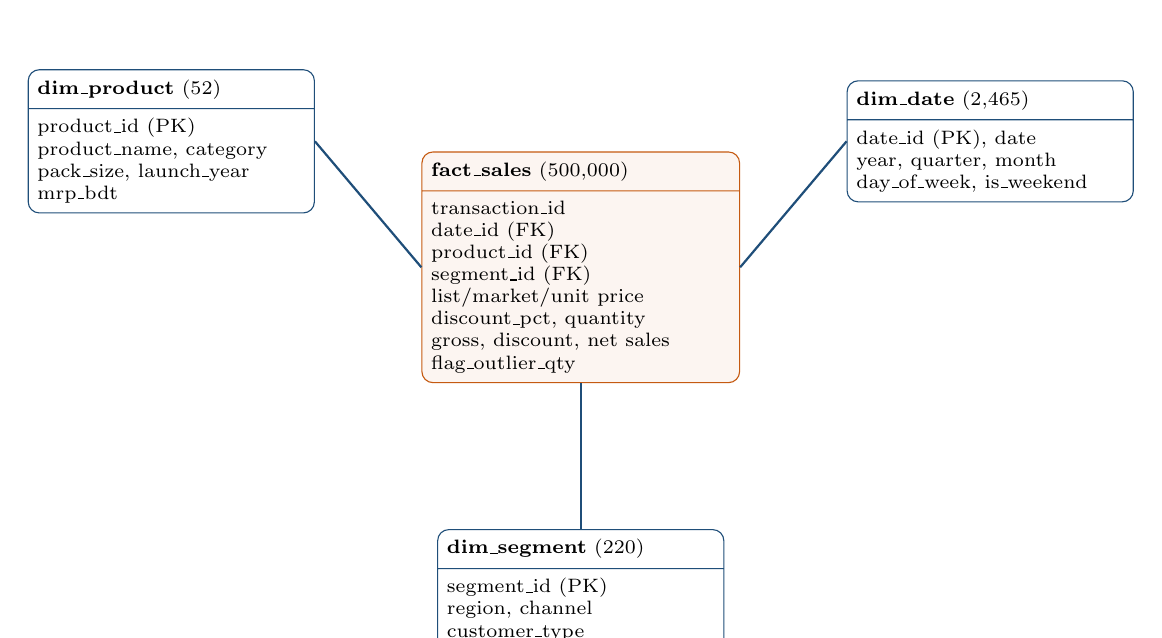
\begin{tikzpicture}[every node/.style={font=\scriptsize},
  T/.style={draw=brand, rectangle split, rectangle split parts=2, rounded corners, fill=white, text width=3.4cm, align=left},
  F/.style={T, draw=accent, fill=accent!6, text width=3.8cm}]
\node[F] (f) at (0,0) {\textbf{fact\_sales} (\NRows)\nodepart{second}transaction\_id\\date\_id (FK)\\product\_id (FK)\\segment\_id (FK)\\list/market/unit price\\discount\_pct, quantity\\gross, discount, net sales\\flag\_outlier\_qty};
\node[T] (p) at (-5.2,1.6) {\textbf{dim\_product} (\NProducts)\nodepart{second}product\_id (PK)\\product\_name, category\\pack\_size, launch\_year\\mrp\_bdt};
\node[T] (d) at (5.2,1.6) {\textbf{dim\_date} (2,465)\nodepart{second}date\_id (PK), date\\year, quarter, month\\day\_of\_week, is\_weekend};
\node[T] (s) at (0,-4.1) {\textbf{dim\_segment} (220)\nodepart{second}segment\_id (PK)\\region, channel\\customer\_type};
\draw[thick, brand] (f.west) -- (p.east); \draw[thick, brand] (f.east) -- (d.west); \draw[thick, brand] (f.south) -- (s.north);
\end{tikzpicture}
\caption{বিশ্লেষণী ডেটাবেসের স্টার স্কিমা}\label{fig:star}
\end{figure}

\chapter{অনুসন্ধানমূলক ডেটা বিশ্লেষণ}\label{ch:eda}

এই অধ্যায় বর্ণনামূলক প্রশ্ন, \emph{কী ঘটেছে?}, এর উত্তর দেয় এবং \emph{কেন} প্রশ্নের উত্তর দেওয়া শুরু করে। সব ফলাফল
\texttt{eda.py} দিয়ে পূর্ণ পরিষ্কার ডেটাসেটে হিসাব করা।

\section{সামগ্রিক কর্মদক্ষতা ও প্রবৃদ্ধি}
পুরো সময়কালে কোম্পানি \NRows টি অর্ডারে \TotalUnits মিলিয়ন ইউনিট বিক্রি করেছে, যার নিট বিক্রয়মূল্য \TotalSales মিলিয়ন টাকা।
গড় অর্ডারের মূল্য ছিল \AOV টাকা, এবং ডিসকাউন্ট গড়ে মোট মূল্যের \AvgDiscount\%, যার মোট খরচ \DiscountCost মিলিয়ন টাকা।
\Cref{tab:annual} ও \cref{fig:trend} স্থির প্রবৃদ্ধি দেখায়। প্রথম ও শেষ পূর্ণ বছরের মধ্যে (2020--2025) নিট বিক্রয় বছরে
\CAGRSales\% চক্রবৃদ্ধি হারে বেড়েছে, এবং জানুয়ারি--সেপ্টেম্বর 2026-এর বিক্রয় 2025-এর একই মাসগুলোর তুলনায় \YTDGrowth\% বেশি।

\begin{table}[htbp]
\centering
\small
\caption{বার্ষিক কর্মদক্ষতার সারসংক্ষেপ, 2020--2026}
\label{tab:annual}
\begin{adjustbox}{max width=\linewidth}
\begin{tabular}{lrrrrrrr}
\toprule
\textbf{Year} & \textbf{Orders} & \textbf{Units} & \textbf{Net sales (BDT M)} & \textbf{AOV (BDT)} & \textbf{Avg price} & \textbf{Disc. \%} & \textbf{YoY \%} \\
\midrule
2020 & 74,788 & 398,005 & 28.62 & 382.7 & 72.0 & 2.34 & -- \\
2021 & 73,636 & 418,104 & 37.02 & 502.7 & 88.6 & 2.35 & +29.3 \\
2022 & 73,898 & 440,150 & 41.00 & 554.8 & 93.4 & 2.34 & +10.8 \\
2023 & 73,598 & 460,465 & 46.17 & 627.3 & 100.5 & 2.36 & +12.6 \\
2024 & 74,282 & 486,293 & 53.03 & 713.9 & 109.8 & 2.35 & +14.9 \\
2025 & 74,442 & 507,262 & 61.78 & 829.9 & 122.3 & 2.35 & +16.5 \\
2026* & 55,356 & 381,678 & 50.75 & 916.8 & 133.8 & 2.34 & -- \\
\bottomrule
\end{tabular}
\end{adjustbox}
\par\smallskip\parbox{0.92\linewidth}{\footnotesize\emph{টীকা:} * 2026 সালে কেবল জানুয়ারি--সেপ্টেম্বর অন্তর্ভুক্ত, তাই এর প্রবৃদ্ধি হিসাব করা হয়নি। AOV = গড় অর্ডার-মূল্য; Avg price = গড় একক বিক্রয়মূল্য।}
\end{table}

\begin{figure}[htbp]\centering
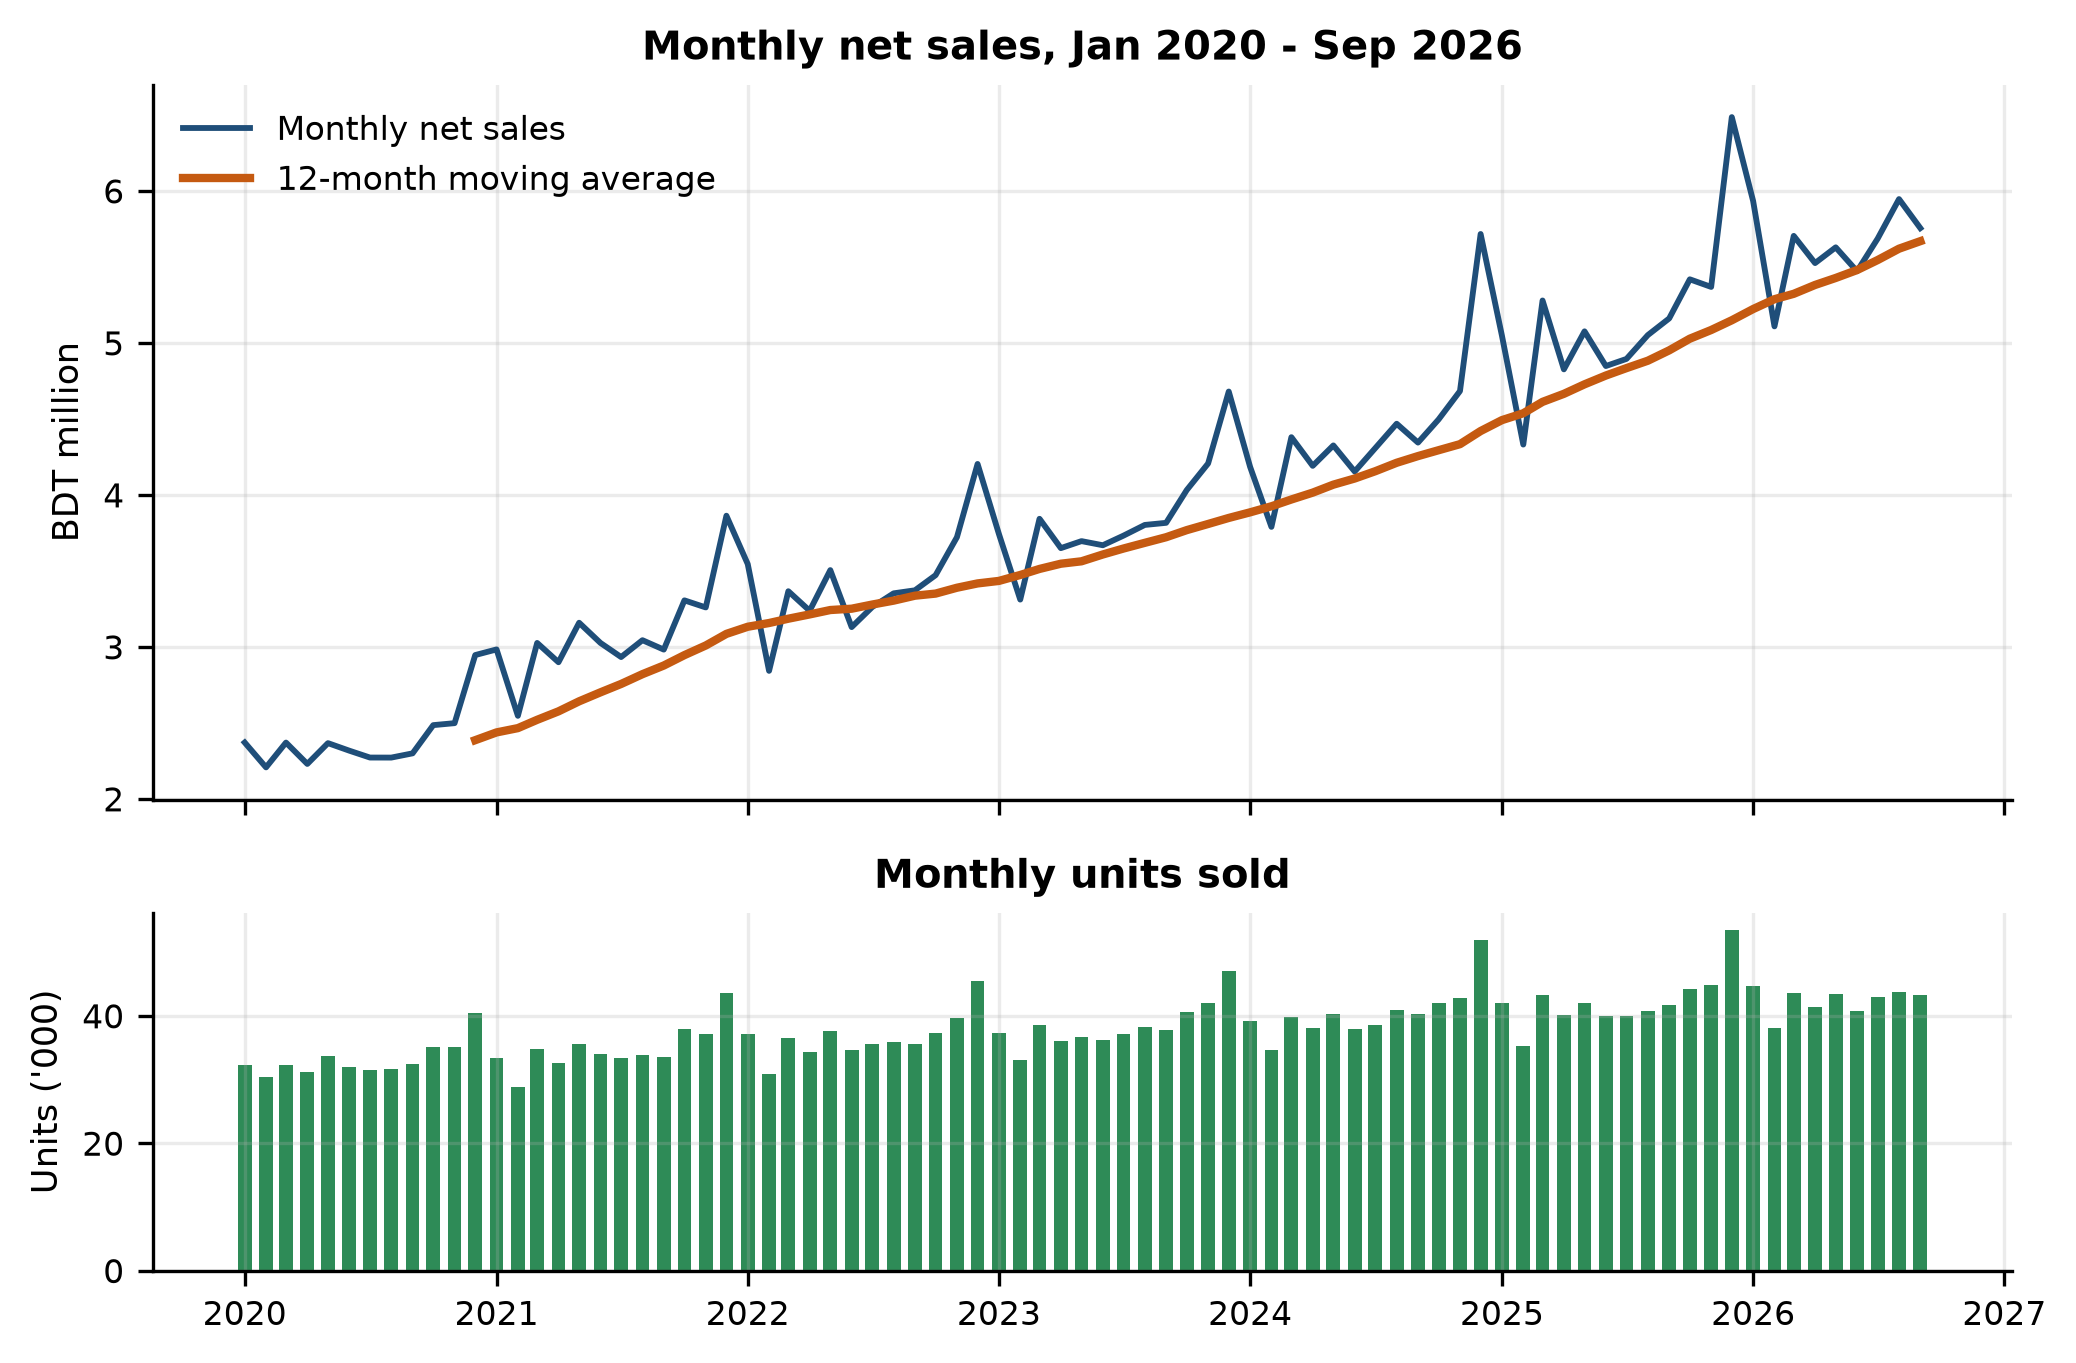
\includegraphics[width=\linewidth]{eda_monthly_trend}
\caption{মাসিক নিট বিক্রয় ও 12-মাসের চলমান গড় (উপরে) এবং মাসিক বিক্রীত ইউনিট (নিচে)}\label{fig:trend}
\end{figure}

\subsection{প্রবৃদ্ধি কোথা থেকে আসে?}
ইউনিট বেড়েছে বছরে মাত্র \CAGRUnits\%, অথচ গড় বিক্রয়মূল্য বেড়েছে বছরে \CAGRPrice\%। বিক্রয় প্রবৃদ্ধিকে হুবহু বিভাজন করা যায়:
$(1+g_{\text{sales}}) = (1+g_{\text{volume}})(1+g_{\text{price}})$। \Cref{tab:pricevolume} ও \cref{fig:pricevolume} দেখায় যে গড়ে
বার্ষিক প্রবৃদ্ধির প্রায় \AvgVolGrowth শতাংশ-বিন্দু এসেছে পরিমাণ থেকে এবং \AvgPriceGrowth এসেছে মূল্য ও পণ্য-মিশ্রণ থেকে। 2021-এর
ব্যতিক্রমী বৃদ্ধি বেশি দামের গিফট বক্স চালুর সঙ্গে মিলে যায় (একটি মিশ্রণ-প্রভাব); পরের বছরগুলো নিয়মিত তালিকা-মূল্য বৃদ্ধির প্রতিফলন।
ব্যবস্থাপনার জন্য এই পার্থক্য গুরুত্বপূর্ণ: মূল্য-নির্ভর প্রবৃদ্ধি অনির্দিষ্টকাল চলতে পারে না, একসময় তা ভোক্তার ক্রয়-সামর্থ্যের সীমায় পৌঁছায়।

\begin{table}[htbp]
\centering
\small
\caption{বার্ষিক বিক্রয় প্রবৃদ্ধির পরিমাণ (volume) ও মূল্য (price) প্রভাবে বিভাজন}
\label{tab:pricevolume}
\begin{adjustbox}{max width=\linewidth}
\begin{tabular}{lrrr}
\toprule
\textbf{Year} & \textbf{Sales growth \%} & \textbf{Volume growth \%} & \textbf{Avg price growth \%} \\
\midrule
2021 & +29.3 & +5.0 & +23.1 \\
2022 & +10.8 & +5.3 & +5.2 \\
2023 & +12.6 & +4.6 & +7.6 \\
2024 & +14.9 & +5.6 & +8.8 \\
2025 & +16.5 & +4.3 & +11.7 \\
\bottomrule
\end{tabular}
\end{adjustbox}
\par\smallskip\parbox{0.92\linewidth}{\footnotesize\emph{টীকা:} $(1+g_{sales}) = (1+g_{volume})(1+g_{price})$; এখানে মূল্য মানে ইউনিটপ্রতি নিট আয়, তাই এতে পণ্য-মিশ্রণের পরিবর্তনও প্রতিফলিত।}
\end{table}

\begin{figure}[htbp]\centering
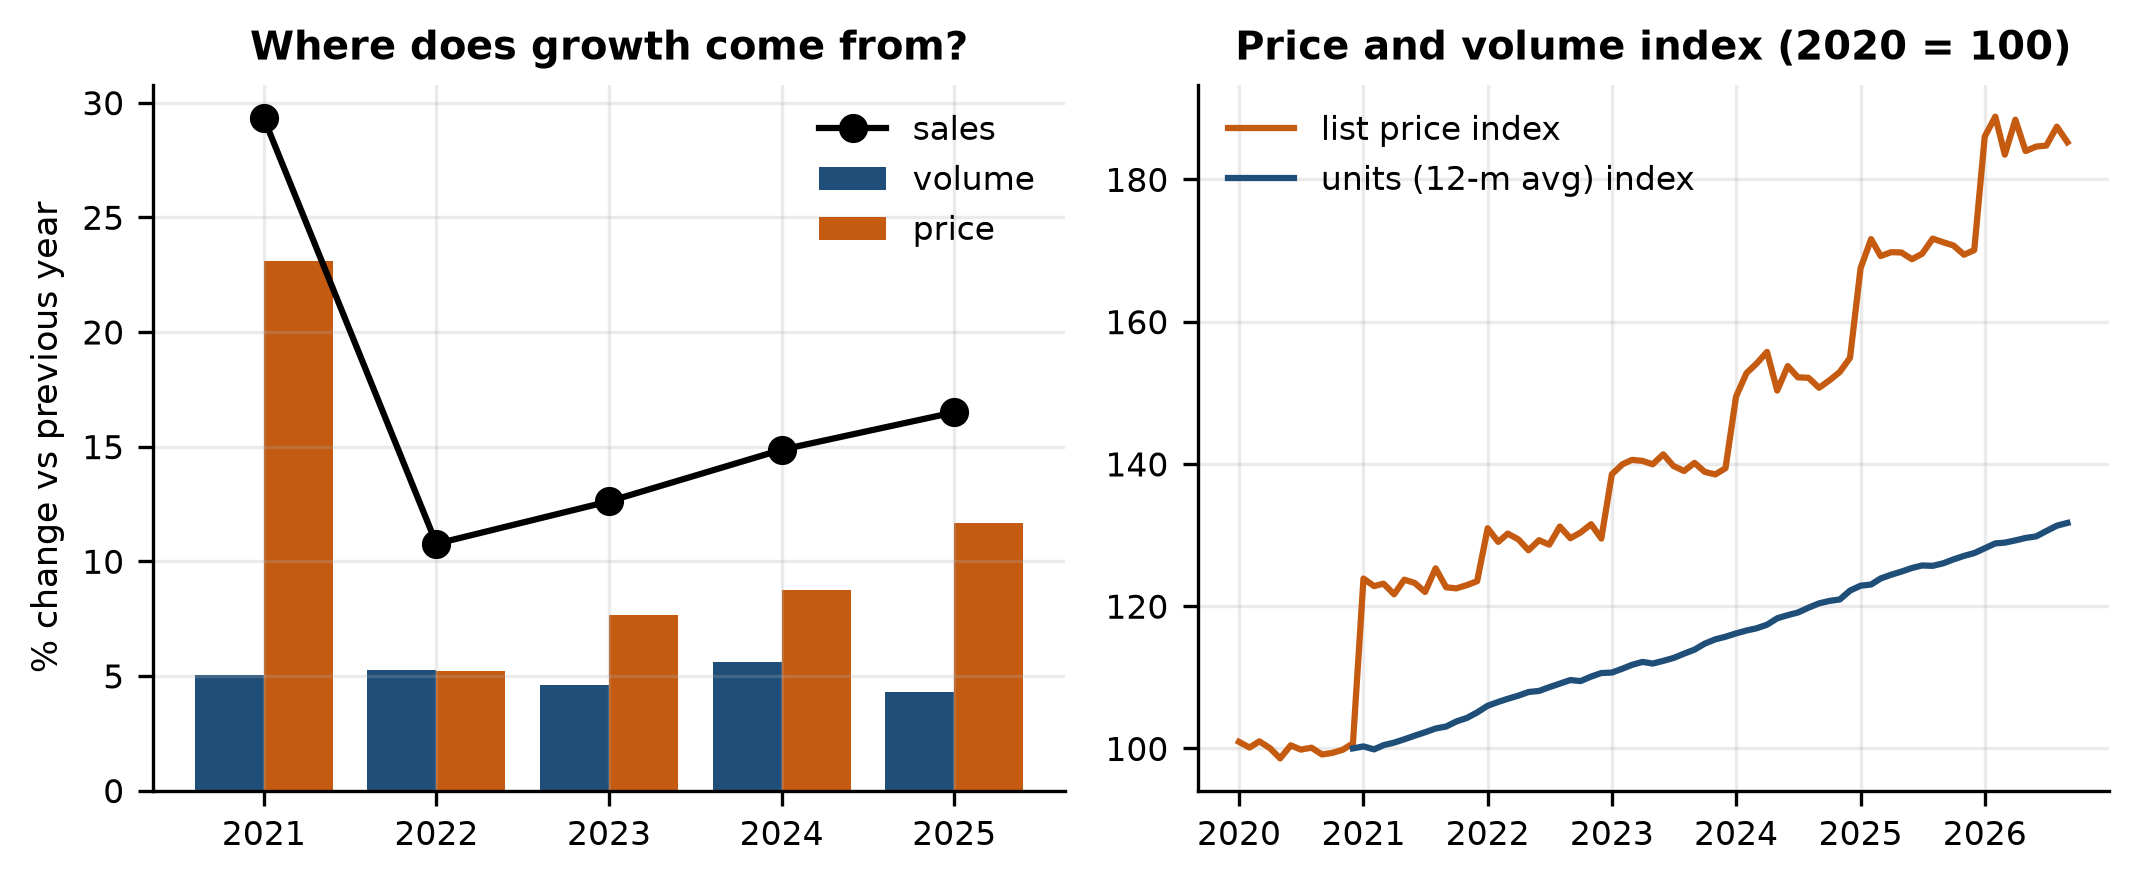
\includegraphics[width=\linewidth]{eda_price_volume}
\caption{প্রবৃদ্ধির বিভাজন (বামে) এবং মূল্য বনাম পরিমাণ সূচক (ডানে)}\label{fig:pricevolume}
\end{figure}

\subsection{চাহিদা কি মূল্য-সংবেদনশীল?}
মূল্যের প্রভাবকে সাধারণ প্রবৃদ্ধি থেকে আলাদা করতে পণ্য-মাস প্যানেলে একটি fixed-effects রিগ্রেশন দিয়ে চাহিদার মূল্য-স্থিতিস্থাপকতা
নির্ণয় করা হয়েছে:
\[
  \log(\text{units}_{pt}) = \beta \log(\text{price}_{pt}) + \alpha_p + \gamma_{\text{year}(t)} + \delta_{\text{month}(t)} + \varepsilon_{pt}.
\]
পণ্য-প্রভাব $\alpha_p$ পণ্যগুলোর আকারের পার্থক্য, বছর-প্রভাব সাধারণ বাজার-প্রবৃদ্ধি এবং মাস-প্রভাব মৌসুমিতা শোষণ করে। নির্ণীত
স্থিতিস্থাপকতা $\hat\beta = \Elasticity$, 95\% আস্থা-ব্যবধান \ElasticityLo থেকে \ElasticityHi (robust standard error;
$p = \ElasticityP$; $R^2 = \ElasticityRtwo$)। এটি শূন্য থেকে তাৎপর্যপূর্ণভাবে আলাদা নয়, অর্থাৎ পর্যবেক্ষিত সীমার মধ্যে চাহিদা
\emph{মূল্য-অস্থিতিস্থাপক}। বছর-প্রভাব ছাড়া একটি সরল রিগ্রেশন বিভ্রান্তিকর \emph{ধনাত্মক} স্থিতিস্থাপকতা (\ElasticityNaive) দেয়,
কারণ সময়ের সঙ্গে মূল্য ও পরিমাণ দুটোই বেড়েছে। এটি confounding-এর একটি পাঠ্যপুস্তকীয় উদাহরণ, এবং এ কারণেই ব্যাখ্যামূলক মডেল
সতর্কভাবে নির্দিষ্ট করতে হয় \citep{shmueli2010}।

\section{মৌসুমিতা ও ক্যালেন্ডারের প্রভাব}
বিক্রয়ে একটি স্পষ্ট বার্ষিক চক্র রয়েছে (\cref{fig:seasonality})। ডিসেম্বর সবচেয়ে শক্তিশালী মাস, মৌসুমি সূচক \PeakIndex
(গড় মাস = 100); অক্টোবর (\OctIndex) ও নভেম্বরও (\NovIndex) গড়ের উপরে, যা বছর-শেষের উৎসব ও উপহারের মৌসুমের সঙ্গে সামঞ্জস্যপূর্ণ।
ফেব্রুয়ারি সবচেয়ে দুর্বল (\TroughIndex)। ফেব্রুয়ারির দুর্বলতার একটি অংশ কেবল এর কম দিনসংখ্যার কারণে: প্রতি কর্মদিবস হিসেবে এর সূচক
\FebPerDay, অথচ ডিসেম্বরের প্রতিদিনের সূচক উচ্চই থাকে (\DecPerDay)। প্রবণতা-মুক্ত দৈনিক বিক্রয়ে Kruskal--Wallis টেস্ট নিশ্চিত করে যে
ক্যালেন্ডারের মাস গুরুত্বপূর্ণ ($H = \KWMonthH$, $p<0.001$)। বিপরীতে সপ্তাহের দিনের প্রভাব প্রায় নেই: সপ্তাহের দিনগুলোর গড় দৈনিক
বিক্রয়ের coefficient of variation মাত্র \DowCV\%।

\begin{figure}[htbp]\centering
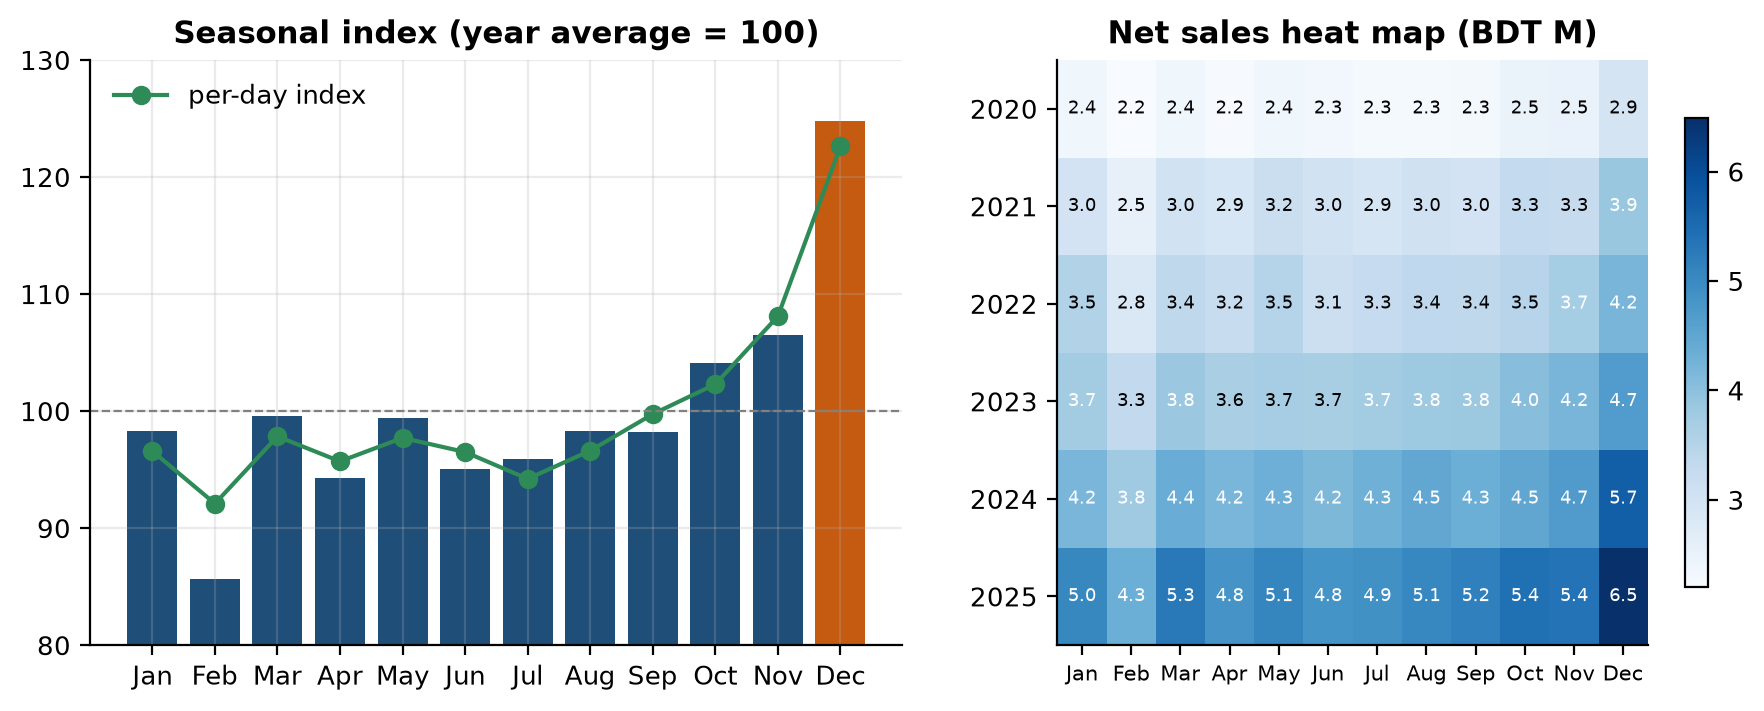
\includegraphics[width=\linewidth]{eda_seasonality}
\caption{মাস অনুযায়ী মৌসুমি সূচক (বামে) এবং বছর $\times$ মাস অনুযায়ী নিট বিক্রয়ের heat map (ডানে)}\label{fig:seasonality}
\end{figure}

\section{পণ্য ও ক্যাটাগরি}
\Cref{tab:category} ও \cref{fig:pareto} ক্যাটাগরি-কাঠামো দেখায়। \TopCategory সবচেয়ে বড় ক্যাটাগরি (বিক্রয়ের \TopCategoryShare\%),
এরপর Pound Cake ও Swiss Roll। Layer Cake-এর প্রবৃদ্ধির হার সর্বোচ্চ (বছরে \FastCategoryCAGR\%), যা মূলত 2021-এ যুক্ত গিফট-বক্স
সংস্করণ থেকে এসেছে; এটি মনে করিয়ে দেয় যে ক্যাটাগরির প্রবৃদ্ধিতে স্বাভাবিক প্রবৃদ্ধি ও পণ্য-পরিসর পরিবর্তন মিশে থাকে। Pareto বিশ্লেষণ
\NProducts টি পণ্যকে ভাগ করে \NClassA টি A-শ্রেণির পণ্যে (যারা আয়ের 80\% আনে), \NClassB টি B-শ্রেণি ও \NClassC টি C-শ্রেণিতে।
সর্বাধিক বিক্রীত দশটি পণ্যই নিট বিক্রয়ের \TopTenShare\% দেয় (\cref{tab:topproducts})।

\begin{table}[htbp]
\centering
\small
\caption{পণ্য-ক্যাটাগরি অনুযায়ী আয় ও প্রবৃদ্ধি}
\label{tab:category}
\begin{adjustbox}{max width=\linewidth}
\begin{tabular}{lrrrr}
\toprule
\textbf{Category} & \textbf{Net sales (BDT M)} & \textbf{Share \%} & \textbf{Products} & \textbf{CAGR 2020-25 \%} \\
\midrule
Muffin & 71.47 & 22.4 & 9 & +32.3 \\
Pound Cake & 61.76 & 19.4 & 12 & +9.7 \\
Swiss Roll & 38.81 & 12.2 & 4 & +9.6 \\
Fruit Cake & 28.90 & 9.1 & 5 & +9.9 \\
Layer Cake & 28.47 & 8.9 & 4 & +67.7 \\
Dry Cake & 25.59 & 8.0 & 3 & +9.4 \\
Cookie & 21.72 & 6.8 & 3 & +11.0 \\
Plain Cake & 16.57 & 5.2 & 6 & +10.4 \\
Velvet Cake & 11.75 & 3.7 & 1 & +10.3 \\
Classic Brownie & 6.27 & 2.0 & 1 & +10.8 \\
Premium & 4.02 & 1.3 & 1 & -- \\
Breakfast & 1.75 & 0.6 & 1 & -- \\
Bread & 1.28 & 0.4 & 2 & -- \\
\bottomrule
\end{tabular}
\end{adjustbox}
\par\smallskip\parbox{0.92\linewidth}{\footnotesize\emph{টীকা:} CAGR প্রথম ও শেষ পূর্ণ বছরের মধ্যে হিসাবকৃত। 2020-এর পরে চালু হওয়া ক্যাটাগরির প্রবৃদ্ধি তাদের চালুর বছর থেকে হিসাব করা।}
\end{table}
\begin{table}[htbp]
\centering
\small
\caption{নিট বিক্রয় অনুযায়ী শীর্ষ দশটি পণ্য (Pareto/ABC বিশ্লেষণ)}
\label{tab:topproducts}
\begin{adjustbox}{max width=\linewidth}
\begin{tabular}{lrrr}
\toprule
\textbf{Product} & \textbf{Net sales (BDT M)} & \textbf{Cumulative share \%} & \textbf{Class} \\
\midrule
MUF007 Cappuccino Muffin Gift Pack & 15.41 & 4.8 & A \\
MUF006 Vanilla Muffin Gift Box & 12.48 & 8.8 & A \\
LAY004 Vanilla Layer Cake Gift Box & 12.44 & 12.7 & A \\
LAY002 Chocolate Layer Cake Gift Box & 12.29 & 16.5 & A \\
MUF003 Chocolate Muffin Gift Box & 12.25 & 20.4 & A \\
MUF009 Chocochips Muffin & 11.99 & 24.1 & A \\
MUF008 Raisin Muffin & 11.80 & 27.8 & A \\
VEL001 Chocolate Velvet Cake & 11.75 & 31.5 & A \\
SWR002 Chocolate Swiss Roll & 11.68 & 35.2 & A \\
SWR004 Strawberry Swiss Roll & 10.44 & 38.5 & A \\
\bottomrule
\end{tabular}
\end{adjustbox}
\end{table}

\begin{figure}[htbp]\centering
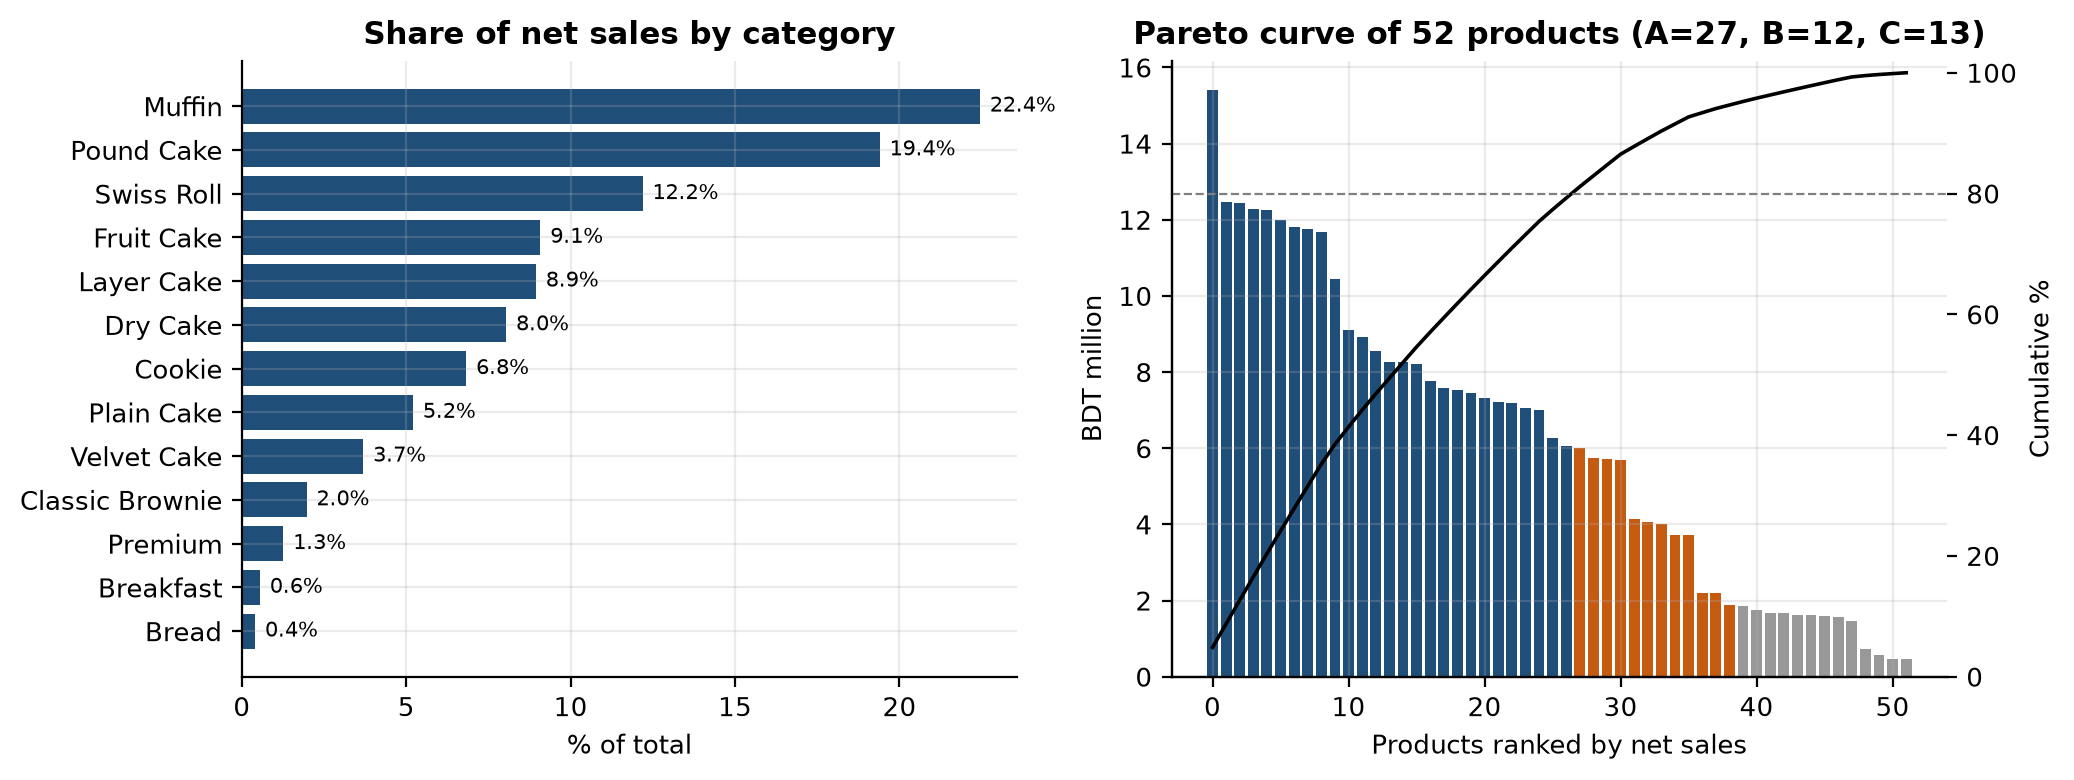
\includegraphics[width=\linewidth]{eda_category_pareto}
\caption{ক্যাটাগরি অনুযায়ী নিট বিক্রয়ের অংশ (বামে) এবং পণ্যের Pareto বক্ররেখা (ডানে)}\label{fig:pareto}
\end{figure}

\section{অঞ্চল, চ্যানেল ও গ্রাহক}
বিক্রয় ভৌগোলিকভাবে কেন্দ্রীভূত। ঢাকা একাই নিট বিক্রয়ের \DhakaShare\% আনে, আর ঢাকা ও চট্টগ্রাম মিলে \DhakaCtgShare\%
(\cref{tab:segments})। General Trade প্রধান চ্যানেল (\GTShare\%), এরপর Modern Trade (\MTShare\%), Distributor (\DistShare\%) ও
E-commerce (\EcomShare\%)। চ্যানেলভেদে অর্ডারের আকারে বড় পার্থক্য: একটি ডিস্ট্রিবিউটর অর্ডারে গড়ে \DistQty ইউনিট, E-commerce অর্ডারে
\EcomQty, General Trade-এ \GTQty এবং Modern Trade-এ \MTQty (\cref{fig:regionchannel})। অন্যদিকে গ্রাহকের ধরন অর্ডারের আকারে কোনো
পার্থক্য আনে না (Kruskal--Wallis $p=\PCustType$), এবং গ্রাহকের ধরনভেদে গড় অর্ডার-মূল্য প্রায় অভিন্ন। অর্থাৎ অর্ডারের আকার নির্ধারণ করে
\emph{বাজারে পৌঁছানোর পথ}, গ্রাহক কে তা নয়।

\begin{table}[htbp]
\centering
\footnotesize
\caption{অঞ্চল, চ্যানেল ও গ্রাহকের ধরন অনুযায়ী কর্মদক্ষতা}
\label{tab:segments}
\begin{adjustbox}{max width=\linewidth}
\begin{tabular}{llrrrrr}
\toprule
\textbf{Dimension} & \textbf{Level} & \textbf{Net sales (BDT M)} & \textbf{Share \%} & \textbf{Orders} & \textbf{AOV (BDT)} & \textbf{Units/order} \\
\midrule
Region & Dhaka & 139.76 & 43.9 & 169,661 & 823.8 & 7.85 \\
Region & Chattogram & 45.89 & 14.4 & 70,440 & 651.4 & 6.33 \\
Region & Gazipur & 25.74 & 8.1 & 39,853 & 645.9 & 6.34 \\
Region & Narayanganj & 21.23 & 6.7 & 35,195 & 603.1 & 5.93 \\
Region & Cumilla & 15.71 & 4.9 & 29,911 & 525.2 & 5.19 \\
Region & Sylhet & 15.27 & 4.8 & 29,901 & 510.6 & 4.92 \\
Region & Rangpur & 12.23 & 3.8 & 30,012 & 407.6 & 4.16 \\
Region & Rajshahi & 12.03 & 3.8 & 25,152 & 478.2 & 4.79 \\
Region & Khulna & 11.73 & 3.7 & 25,094 & 467.3 & 4.71 \\
Region & Mymensingh & 10.76 & 3.4 & 24,849 & 432.9 & 4.34 \\
Region & Barishal & 8.04 & 2.5 & 19,932 & 403.2 & 3.96 \\
Channel & General Trade & 145.21 & 45.6 & 260,431 & 557.6 & 5.32 \\
Channel & Modern Trade & 81.55 & 25.6 & 124,619 & 654.4 & 6.28 \\
Channel & Distributor & 72.90 & 22.9 & 64,861 & 1,123.9 & 11.43 \\
Channel & E-commerce & 18.72 & 5.9 & 50,089 & 373.7 & 3.66 \\
Customer type & Retailer & 143.28 & 45.0 & 224,582 & 638.0 & 6.19 \\
Customer type & Super Shop & 63.31 & 19.9 & 100,073 & 632.7 & 6.16 \\
Customer type & Distributor & 47.91 & 15.0 & 75,413 & 635.3 & 6.19 \\
Customer type & Online Customer & 31.95 & 10.0 & 49,759 & 642.0 & 6.17 \\
Customer type & Corporate & 31.93 & 10.0 & 50,173 & 636.4 & 6.21 \\
\bottomrule
\end{tabular}
\end{adjustbox}
\end{table}

\begin{figure}[htbp]\centering
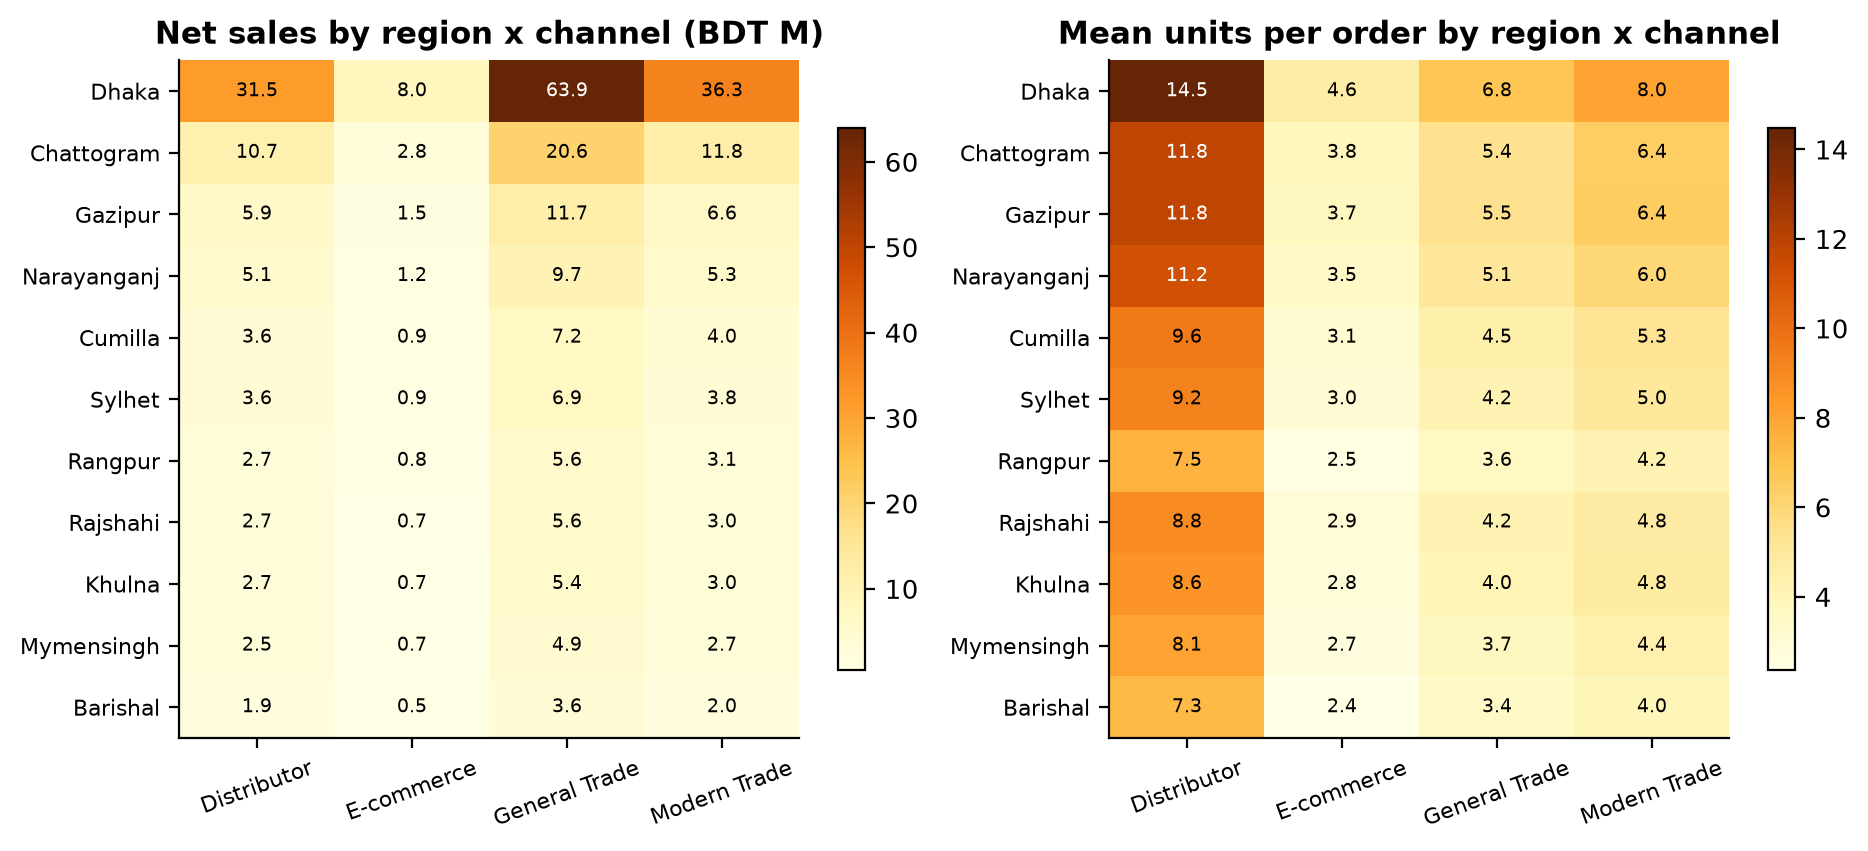
\includegraphics[width=\linewidth]{eda_region_channel}
\caption{অঞ্চল ও চ্যানেল অনুযায়ী নিট বিক্রয় (বামে) এবং অর্ডারপ্রতি গড় ইউনিট (ডানে)}\label{fig:regionchannel}
\end{figure}

\section{বণ্টন ও সম্পর্ক}
অর্ডারের পরিমাণ ও অর্ডার-মূল্য তীব্রভাবে ডানদিকে বিষম, skewness যথাক্রমে \QtySkew ও \ValueSkew (\cref{fig:distributions}):
অধিকাংশ অর্ডার ছোট, এবং বাল্ক অর্ডারের একটি দীর্ঘ লেজ আছে। এই আকৃতিই বিশ্লেষণ জুড়ে median, rank-ভিত্তিক টেস্ট ও log রূপান্তর
ব্যবহারের যৌক্তিকতা দেয়। Spearman সম্পর্ক-ম্যাট্রিক্স (\cref{fig:correlation}) দেখায় যে অর্ডার-মূল্য পরিমাণ ($\rho=\CorrSalesQty$) ও
মূল্য ($\rho=\CorrSalesPrice$) উভয় দিয়েই চালিত, কিন্তু পরিমাণ ও মূল্য কার্যত সম্পর্কহীন ($\rho=\CorrQtyPrice$): গ্রাহকরা বেশি দামের
পণ্যের কম প্যাক কেনেন না।

\begin{figure}[htbp]\centering
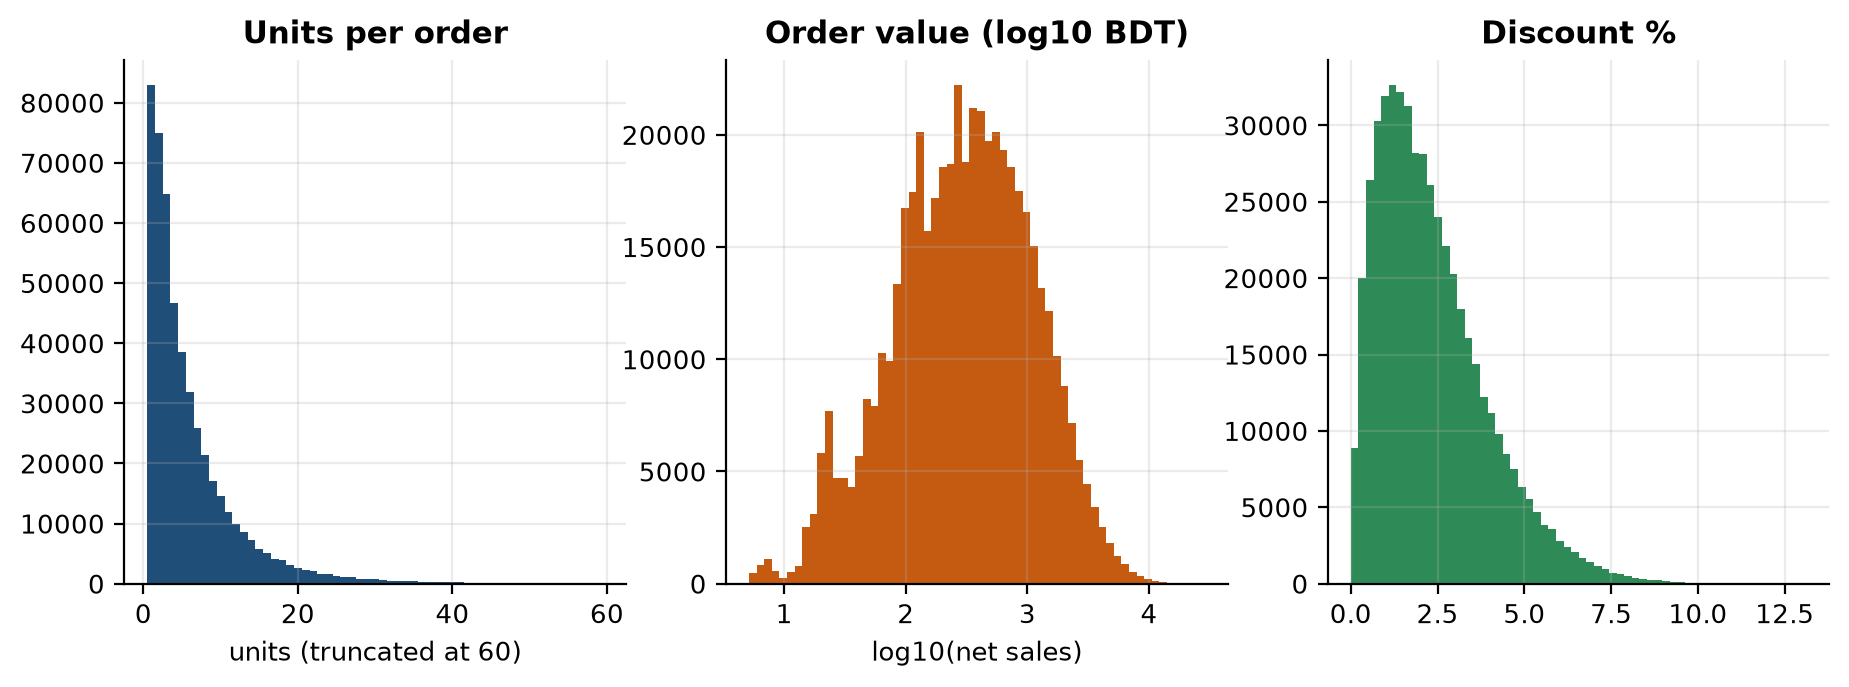
\includegraphics[width=\linewidth]{eda_distributions}
\caption{অর্ডারপ্রতি ইউনিট, অর্ডার-মূল্য (log স্কেল) ও ডিসকাউন্টের বণ্টন}\label{fig:distributions}
\end{figure}

\begin{figure}[htbp]\centering
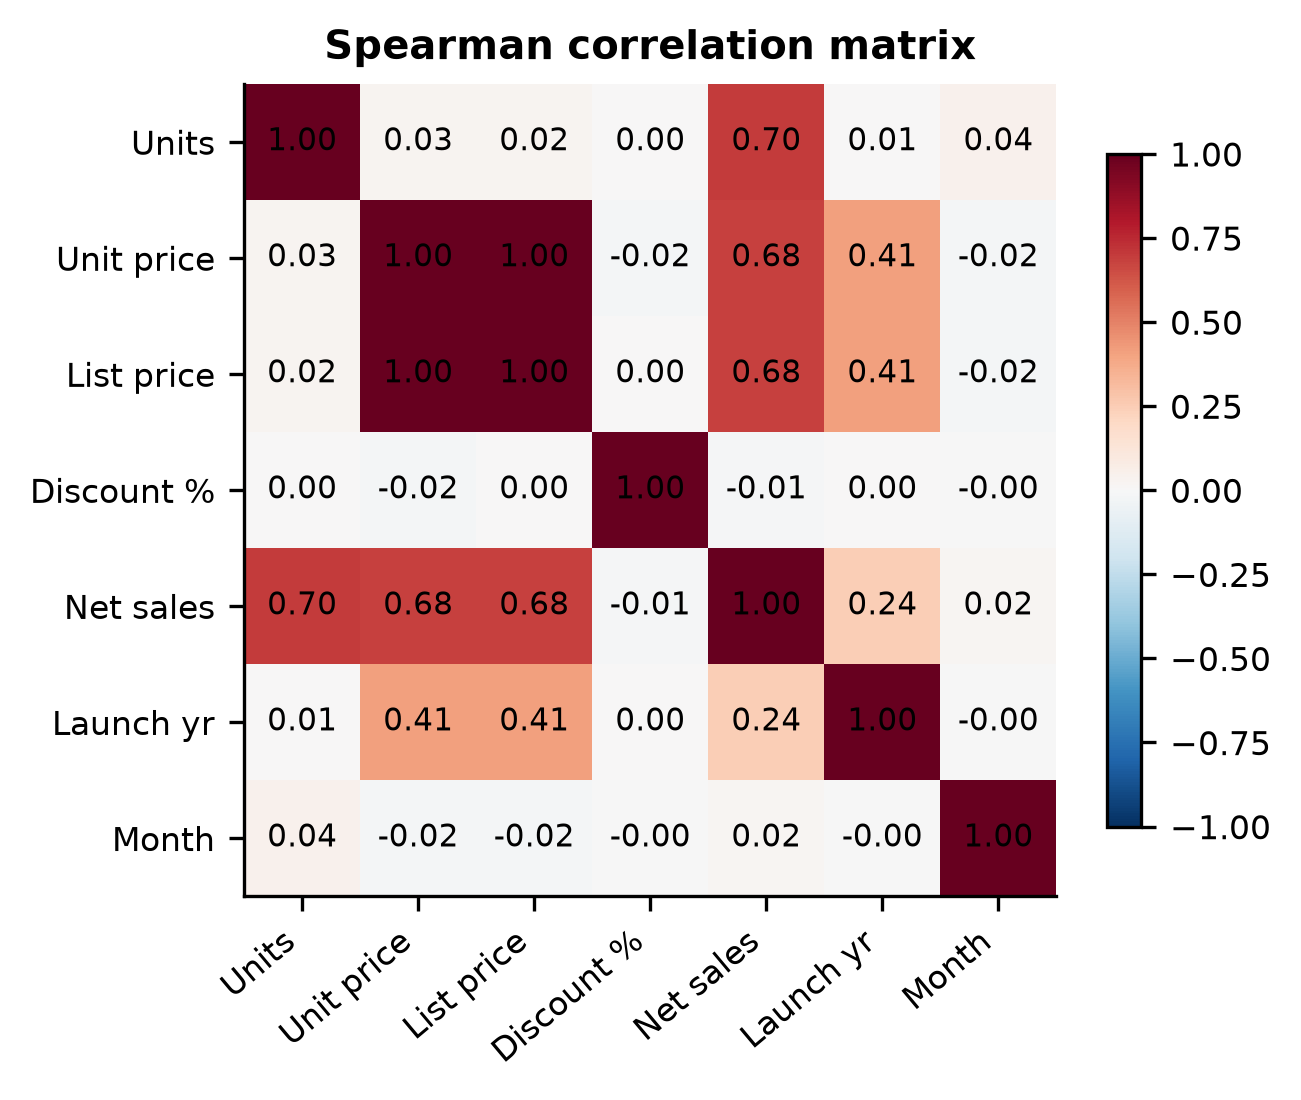
\includegraphics[width=.62\linewidth]{eda_correlation}
\caption{প্রধান সংখ্যাসূচক চলকগুলোর Spearman সম্পর্ক-ম্যাট্রিক্স}\label{fig:correlation}
\end{figure}

\section{হাইপোথিসিস টেস্ট}
\Cref{tab:tests} প্রধান অনুসন্ধানমূলক ফলাফলগুলোকে আনুষ্ঠানিক রূপ দেয়। পাঁচ লক্ষ পর্যবেক্ষণে দুটি বাদে সব পার্থক্যই পরিসংখ্যানিকভাবে
তাৎপর্যপূর্ণ, তাই ব্যাখ্যার জন্য effect size অপরিহার্য। অর্ডারের আকারের সবচেয়ে বেশি পরিবর্তন ব্যাখ্যা করে চ্যানেল
($\varepsilon^2=\EpsChannel$), তারপর অঞ্চল ($\varepsilon^2=\EpsRegion$)। চ্যানেল ও বড় অর্ডারের সম্পর্ক মাঝারি (Cram\'er's
$V=\CramerV$)। ডিসকাউন্টের গভীরতা ও অর্ডারের আকার \emph{সম্পর্কহীন} ($\rho=\RhoDisc$, $p=\PDisc$): প্রদত্ত ডিসকাউন্ট বড় কেনাকাটায়
উৎসাহ দেয় বলে মনে হয় না। এটি একটি সম্ভাব্য মূল্যবান ফলাফল, কারণ এই সময়কালে ডিসকাউন্টে কোম্পানির খরচ হয়েছে \DiscountCost মিলিয়ন টাকা।

\begin{table}[htbp]
\centering
\small
\caption{প্রধান অনুসন্ধানমূলক হাইপোথিসিসের পরিসংখ্যানিক টেস্ট}
\label{tab:tests}
\begin{adjustbox}{max width=\linewidth}
\begin{tabular}{llrrr}
\toprule
\textbf{Hypothesis (H0: no difference)} & \textbf{Test} & \textbf{Statistic} & \textbf{p-value} & \textbf{Effect size} \\
\midrule
Units/order by channel & Kruskal-Wallis & 43,269.88 & <0.001 & 0.0865 \\
Units/order by region & Kruskal-Wallis & 27,261.36 & <0.001 & 0.0545 \\
Units/order by customer type & Kruskal-Wallis & 2.62 & 0.623 & -0.0000 \\
Daily sales by month (detrended) & Kruskal-Wallis & 510.92 & <0.001 & 0.2293 \\
Discount \% vs units/order & Spearman rho & 0.00 & 0.479 & 0.0000 \\
Large order vs channel & Chi-square & 31,777.06 & <0.001 & 0.2521 \\
\bottomrule
\end{tabular}
\end{adjustbox}
\par\smallskip\parbox{0.92\linewidth}{\footnotesize\emph{টীকা:} Effect size: Kruskal--Wallis-এর জন্য $\varepsilon^2$, Spearman-এর জন্য $\rho^2$ এবং chi-square-এর জন্য Cram\'er's $V$। $n=500{,}000$ হলে প্রায় যেকোনো পার্থক্যই `তাৎপর্যপূর্ণ', তাই ব্যবহারিক গুরুত্ব বিচার করে effect size।}
\end{table}

\section{অনুসন্ধানমূলক ফলাফলের সারসংক্ষেপ}
\begin{enumerate}
  \item আয়ের প্রবৃদ্ধি শক্তিশালী (বছরে \CAGRSales\%) কিন্তু মূলত মূল্য ও মিশ্রণ-চালিত; পরিমাণ বাড়ছে \CAGRUnits\% হারে।
  \item পর্যবেক্ষিত সীমায় চাহিদা মূল্য-অস্থিতিস্থাপক, এবং ডিসকাউন্টের অর্ডারের আকারে কোনো পরিমাপযোগ্য প্রভাব নেই।
  \item মৌসুমিতা স্পষ্ট: ডিসেম্বরে শীর্ষ ও ফেব্রুয়ারিতে সর্বনিম্ন; সপ্তাহের দিনের প্রভাব নেই।
  \item আয় কেন্দ্রীভূত: ঢাকা বিক্রয়ের \DhakaShare\% এবং দশটি পণ্য \TopTenShare\% দেয়।
  \item অর্ডারের আকার নির্ভর করে চ্যানেল ও অঞ্চলের উপর, গ্রাহকের ধরনের উপর নয়।
\end{enumerate}
এই ফলাফলগুলো পরের অধ্যায়ের মডেলিং সিদ্ধান্তে কাজে লেগেছে: পূর্বাভাসে মৌসুমিতা ও ইতিহাস-ফিচার, ক্লাসিফিকেশনে চ্যানেল ও অঞ্চল, এবং
বিভাজনে মূল্য, প্রবৃদ্ধি ও মৌসুমিতা।

\chapter{পূর্বাভাসমূলক মডেলিং ও মূল্যায়ন}\label{ch:models}

এই অধ্যায় পূর্বাভাসমূলক প্রশ্ন, \emph{সামনে কী ঘটতে পারে?}, এর উত্তর দেয়। এখানে পর্যায়ক্রমে চারটি বিশ্লেষণী সমস্যা আলোচিত: চাহিদা
পূর্বাভাস, বড় অর্ডারের ক্লাসিফিকেশন, বিভাজন এবং অ্যানোমালি ডিটেকশন।

\section{মাসিক চাহিদা পূর্বাভাস}
\subsection{প্রস্তুতি}
পূর্বাভাস প্যানেলে মাসিকভাবে পর্যবেক্ষিত \PanelSeries টি পণ্য রয়েছে। প্রশিক্ষণ-সারি \PanelTrain টি (2020--2024) এবং পরীক্ষা-সারি
\PanelTest টি (জানুয়ারি 2025 -- সেপ্টেম্বর 2026)। প্রতিটি মডেল $\log(1+\text{units})$ পূর্বাভাস করে, যা পরে ইউনিটে রূপান্তরিত হয়।
Log স্কেল চাহিদার গুণাত্মক প্রকৃতির সঙ্গে মানানসই এবং সবচেয়ে বড় পণ্যগুলোকে fit-এ আধিপত্য করতে দেয় না। সাতটি অ্যালগরিদম
\cref{ch:method}-এ বর্ণিত expanding-window ভাঁজে randomised search দিয়ে টিউন করা হয়েছে; নির্বাচিত hyper-parameter
\cref{app:hyper}-এর \cref{tab:hyper}-এ দেওয়া আছে।

\subsection{এক-ধাপ-অগ্রিম ফলাফল}
\Cref{tab:forecast} পরীক্ষাকালের কর্মদক্ষতা দেখায় যখন প্রতিটি মাস আগের মাস পর্যন্ত প্রকৃত ইতিহাস দিয়ে পূর্বাভাস করা হয়, অর্থাৎ মাসিক
পরিকল্পনা-চক্রের বাস্তব পরিস্থিতি। প্রতিটি মেশিন লার্নিং মডেল দুটি naive বেঞ্চমার্ককেই স্পষ্টভাবে হারিয়েছে। সেরা মডেল \BestReg-এর
RMSE \BestRegRMSE ইউনিট, WAPE \BestRegWAPE\% এবং $R^2=\BestRegRtwo$; অর্থাৎ seasonal-naive নিয়মের (\SNaiveRMSE) চেয়ে RMSE
\GainVsSNaive\% কম এবং naive নিয়মের (\NaiveRMSE) চেয়ে \GainVsNaive\% কম।

\begin{table}[htbp]
\centering
\footnotesize
\caption{মাসিক পণ্য-চাহিদা পূর্বাভাস: পরীক্ষাকালের কর্মদক্ষতা (এক-ধাপ-অগ্রিম, জানুয়ারি 2025--সেপ্টেম্বর 2026)}
\label{tab:forecast}
\begin{adjustbox}{max width=\linewidth}
\begin{tabular}{lrrrrrrrr}
\toprule
\textbf{Model} & \textbf{MAE} & \textbf{MSE} & \textbf{RMSE} & \textbf{R$^2$} & \textbf{MAPE \%} & \textbf{WAPE \%} & \textbf{CV RMSE} & \textbf{Fit (s)} \\
\midrule
Seasonal naive (same month last year) & 120.0 & 23,233 & 152.4 & 0.551 & 15.38 & 14.74 & -- & 0.0 \\
Naive (last month) & 139.8 & 31,051 & 176.2 & 0.400 & 18.00 & 17.17 & -- & 0.0 \\
Support Vector Regression & 90.6 & 13,271 & 115.2 & 0.744 & 12.26 & 11.13 & 0.2151 & 20.0 \\
Linear Regression & 91.3 & 13,861 & 117.7 & 0.732 & 11.48 & 11.21 & 0.1691 & 0.4 \\
XGBoost & 93.3 & 14,294 & 119.6 & 0.724 & 12.28 & 11.46 & 0.1917 & 103.3 \\
Random Forest & 93.0 & 14,413 & 120.1 & 0.722 & 12.04 & 11.42 & 0.1918 & 142.2 \\
Gradient Boosting & 95.7 & 15,113 & 122.9 & 0.708 & 12.51 & 11.76 & 0.1889 & 108.6 \\
K-Nearest Neighbors & 97.0 & 15,865 & 126.0 & 0.694 & 12.01 & 11.91 & 0.1951 & 8.4 \\
Decision Tree & 103.6 & 17,978 & 134.1 & 0.653 & 13.70 & 12.73 & 0.2077 & 7.2 \\
\bottomrule
\end{tabular}
\end{adjustbox}
\par\smallskip\parbox{0.92\linewidth}{\footnotesize\emph{টীকা:} ত্রুটি প্রতি পণ্য-মাসে ইউনিটে। CV RMSE হলো টিউনিংয়ে ব্যবহৃত 2022, 2023 ও 2024-এর expanding-window ভাঁজে log স্কেলে গড় validation RMSE। বেসলাইনের কোনো fitting লাগে না।}
\end{table}

আরও তিনটি পর্যবেক্ষণ উল্লেখযোগ্য। প্রথমত, ভালো মডেলগুলোর পার্থক্য সামান্য: RMSE \BestRegRMSE থেকে \WorstRegRMSE ইউনিটের মধ্যে,
এবং log-ফিচারে linear regression (\LinRMSE) tree ensemble-এর (random forest \RFRMSE, XGBoost \XGBRMSE) সঙ্গে প্রতিযোগিতামূলক।
ভালো lag ও মৌসুমি ফিচার থাকলে সমস্যাটি মূলত log-linear হয়ে যায়, ফলে মডেলের জটিলতা সামান্যই যোগ করে; এটি
\citet{makridakis2018}-এর সঙ্গে সামঞ্জস্যপূর্ণ। দ্বিতীয়ত, একক decision tree সবচেয়ে দুর্বল (\DTRMSE), যা এর উচ্চ ভেদাঙ্কের কারণে
প্রত্যাশিত; একটি forest-এ অনেক tree-র গড় নিলে এই দুর্বলতার বেশিরভাগ দূর হয় \citep{breiman2001}। তৃতীয়ত, প্রশিক্ষণ-বছরের
cross-validated স্কোর মডেলগুলোকে পরীক্ষা-স্কোরের মতোই ক্রমে সাজায়, তাই যাচাই-নকশাটি ভবিষ্যৎ কর্মদক্ষতার নির্ভরযোগ্য নির্দেশক।
\Cref{fig:forecastcomp} মডেলগুলোর তুলনা করে এবং দেখায় যে ভিন্ন আকারের পণ্যেও \BestReg-এর পূর্বাভাস প্রকৃত মানের খুব কাছাকাছি।

\begin{figure}[htbp]\centering
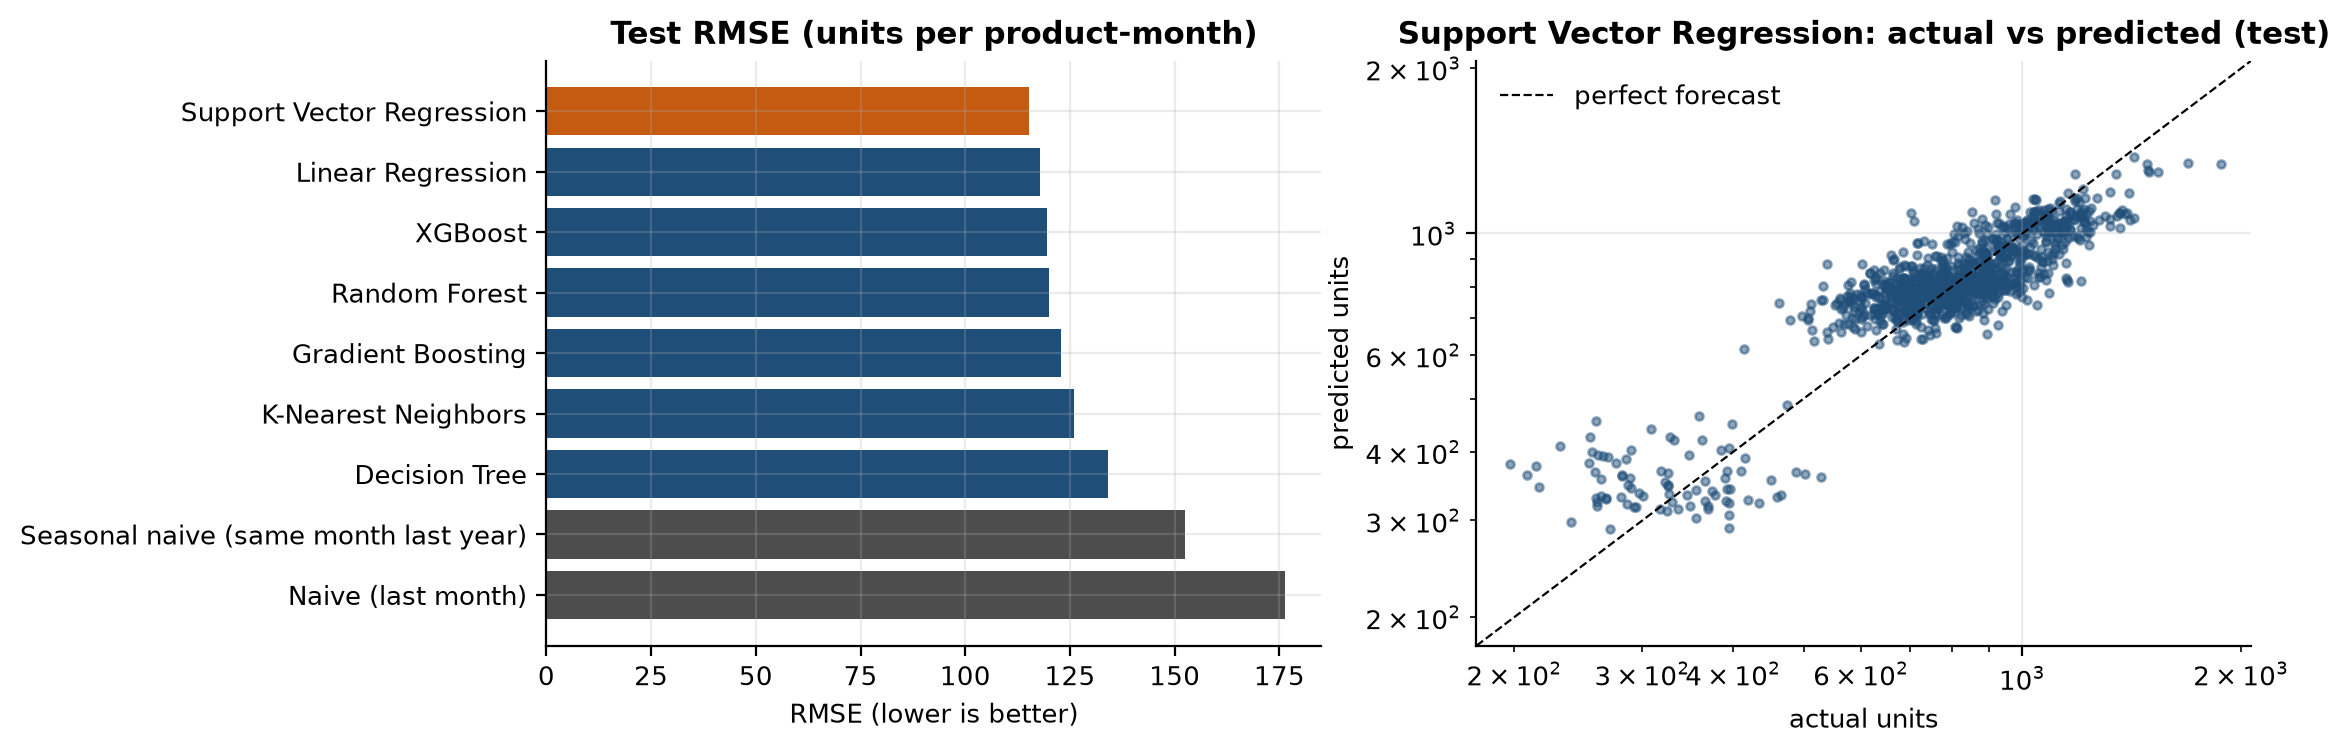
\includegraphics[width=\linewidth]{ml_forecast_comparison}
\caption{সব পূর্বাভাস মডেলের পরীক্ষা-RMSE (বামে; সেরা মডেল চিহ্নিত, বেসলাইন ধূসর) এবং সেরা মডেলের প্রকৃত বনাম পূর্বাভাসিত ইউনিট (ডানে)}\label{fig:forecastcomp}
\end{figure}

\subsection{Recursive বহু-ধাপ ফলাফল}
একটি কঠিনতর পরীক্ষা হলো ডিসেম্বর 2024 থেকে প্রশিক্ষণের পরে কোনো প্রকৃত ডেটা \emph{না দেখে} সব 21টি পরীক্ষা-মাসের পূর্বাভাস দেওয়া,
যেখানে প্রতিটি মাসের পূর্বাভাস পরের মাসের ইতিহাস হিসেবে ফিরে আসে; এটি বার্ষিক বাজেটের পরিস্থিতি। \Cref{tab:recursive} দেখায় যে সেরা
মডেলগুলোর অবনতি সামান্য: \BestRec-এর WAPE \BestRecWAPE\% ($R^2=\BestRecRtwo$), যা 2024-এর প্যাটার্ন পুনরাবৃত্তির চেয়ে অনেক ভালো।
Recursion-এ XGBoost-এর অবনতি সবচেয়ে বেশি: যখন মডেলের নিজের পূর্বাভাস ইনপুট হয় তখন ত্রুটি জমা হয়, এবং প্রশিক্ষণ ডেটায় ঘনিষ্ঠভাবে
fit করা boosted tree এতে বেশি ক্ষতিগ্রস্ত হয়।

\begin{table}[htbp]
\centering
\small
\caption{ডিসেম্বর 2024 থেকে recursive 21-মাসের পূর্বাভাস (প্রশিক্ষণের পরে কোনো প্রকৃত ডেটা ব্যবহৃত হয়নি)}
\label{tab:recursive}
\begin{adjustbox}{max width=\linewidth}
\begin{tabular}{lrrrrr}
\toprule
\textbf{Model} & \textbf{MAE} & \textbf{RMSE} & \textbf{R$^2$} & \textbf{MAPE \%} & \textbf{WAPE \%} \\
\midrule
Random Forest & 91.0 & 117.0 & 0.736 & 11.85 & 11.18 \\
Support Vector Regression & 92.3 & 117.2 & 0.735 & 12.65 & 11.34 \\
Linear Regression & 94.1 & 121.4 & 0.715 & 11.73 & 11.56 \\
XGBoost & 104.1 & 137.5 & 0.635 & 16.17 & 12.79 \\
Seasonal naive (2024 pattern repeated) & 125.9 & 158.1 & 0.517 & 15.87 & 15.47 \\
\bottomrule
\end{tabular}
\end{adjustbox}
\end{table}

\subsection{কোম্পানি-পর্যায়ের পূর্বাভাস ও মডেল মিলকরণ}
পণ্যের পূর্বাভাস যোগ করে কোম্পানির মোট পাওয়া যায়, যা সরাসরি মোট সিরিজে fit করা পরিসংখ্যানিক মডেলের সঙ্গে তুলনা করা যায়
(\cref{tab:company}, \cref{fig:companyfc})। এই সমষ্টিগত পর্যায়ে additive প্রবণতা ও multiplicative মৌসুমিতাসহ Holt--Winters মডেল
সবচেয়ে নির্ভুল, MAPE মাত্র \HWMAPE\%। যোগ করা মেশিন লার্নিং পূর্বাভাসও নির্ভুল, তবে সামান্য কম। এটি সাহিত্যের সঙ্গে সামঞ্জস্যপূর্ণ:
মসৃণ সমষ্টিগত সিরিজে পরিসংখ্যানিক মডেল সুবিধা পায়, আর পৃথক পণ্যের স্তরে মেশিন লার্নিংয়ের সমন্বিত-শিক্ষণ সুবিধা কাজে লাগে। তাই
কাঠামোটি দুটিকে \emph{top-down reconciliation} দিয়ে একত্র করে \citep{athanasopoulos2009}: Holt--Winters কোম্পানির মোট ও তার
পূর্বাভাস-ব্যবধান নির্ধারণ করে, আর মেশিন লার্নিং মডেল সেই মোটকে পণ্যগুলোর মধ্যে বণ্টন করে, যাতে পণ্য-পরিকল্পনা হুবহু কোম্পানি-পরিকল্পনার
সমান হয়।

\begin{table}[htbp]
\centering
\small
\caption{কোম্পানি-স্তরের মাসিক ইউনিট পূর্বাভাস, পরীক্ষাকাল জানুয়ারি 2025--সেপ্টেম্বর 2026}
\label{tab:company}
\begin{adjustbox}{max width=\linewidth}
\begin{tabular}{lrrr}
\toprule
\textbf{Model (company-total monthly units)} & \textbf{MAE} & \textbf{RMSE} & \textbf{MAPE \%} \\
\midrule
Holt-Winters (additive trend, multiplicative season) & 559 & 698 & 1.32 \\
SARIMA(1,1,1)(0,1,1)$_{12}$ on log units & 687 & 806 & 1.65 \\
Support Vector Regression one-step, summed over products & 712 & 875 & 1.68 \\
Random Forest recursive, summed over products & 1,186 & 1,386 & 2.77 \\
Seasonal naive (2024 repeated) & 2,549 & 2,817 & 6.00 \\
\bottomrule
\end{tabular}
\end{adjustbox}
\end{table}

\begin{figure}[htbp]\centering
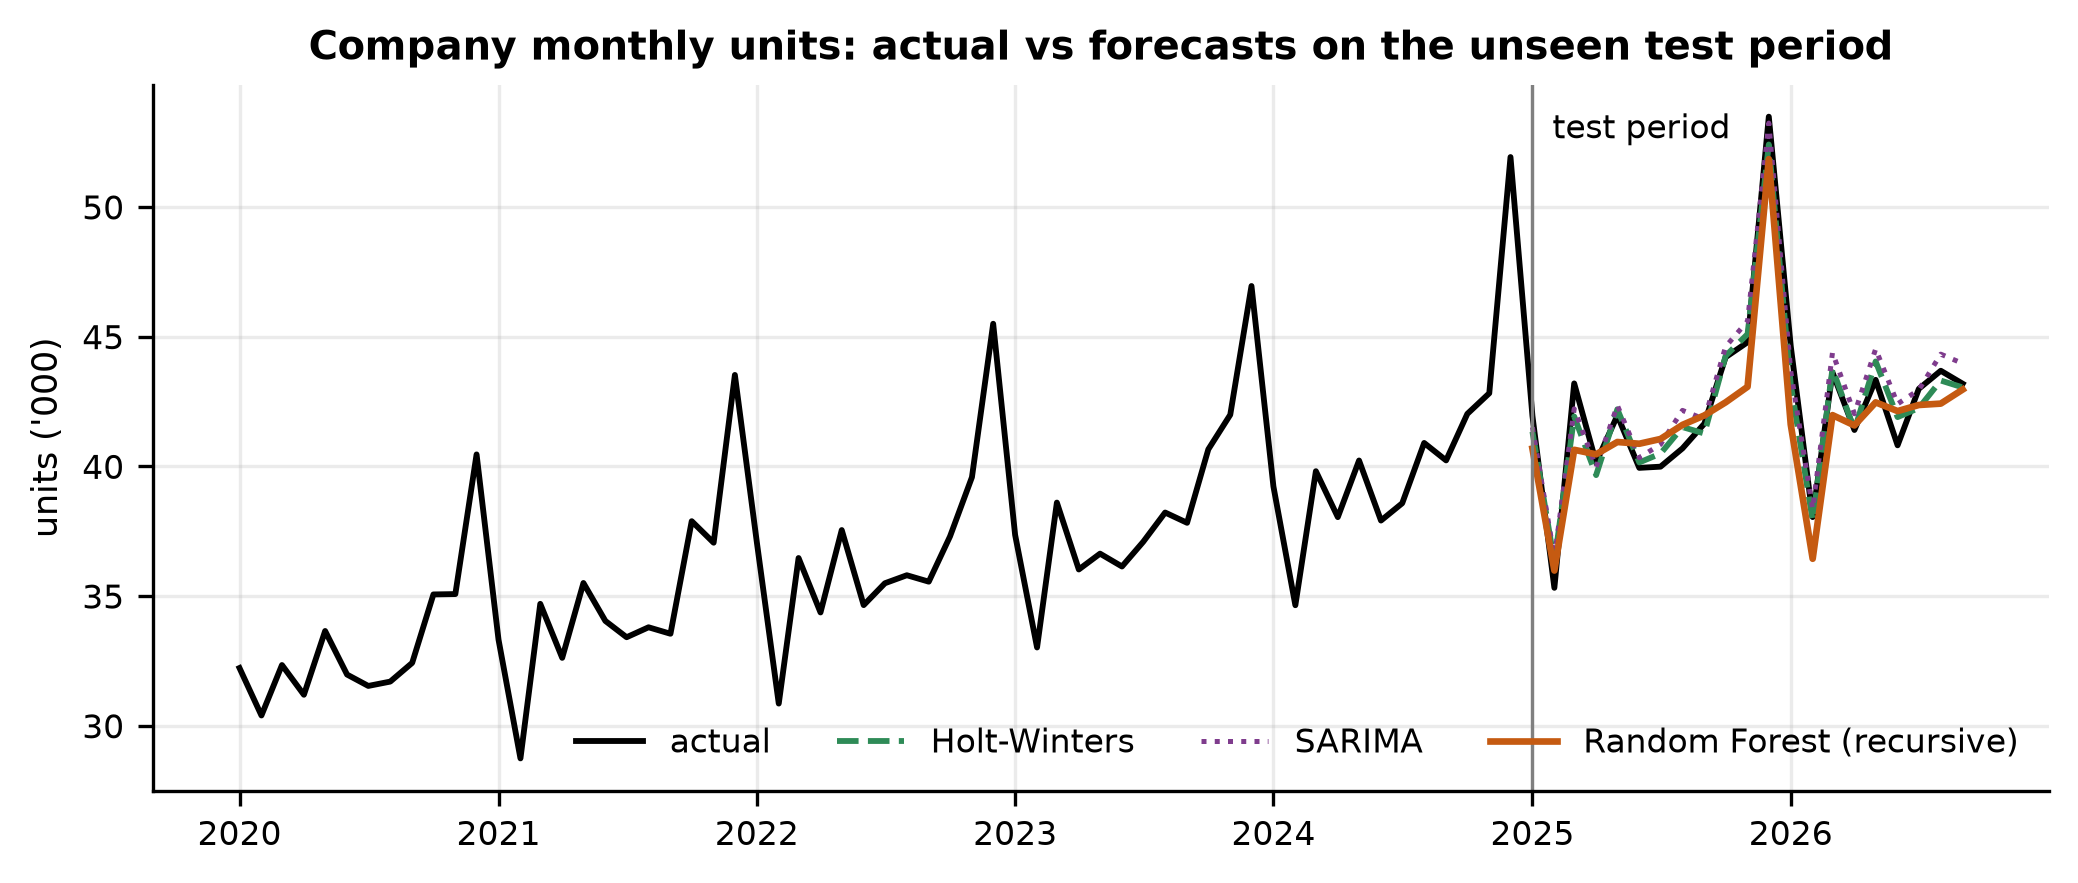
\includegraphics[width=\linewidth]{ml_company_forecast_test}
\caption{কোম্পানির মাসিক ইউনিট: পরীক্ষাকালে প্রকৃত মান ও প্রতিযোগী পূর্বাভাস}\label{fig:companyfc}
\end{figure}

\subsection{পূর্বাভাসের চালিকাশক্তি কী?}
\Cref{fig:importance} মডেলগুলো ব্যাখ্যা করে। \BestReg-এর permutation importance দেখায় যে সাম্প্রতিক ইতিহাস (lag ও rolling গড়)
সবচেয়ে বেশি তথ্য বহন করে, তারপর মৌসুমি ফিচার। XGBoost-এর SHAP মানও একই চিত্র দেয় এবং ডিসেম্বর-সূচক ও 12-মাসের lag-কে তুলে ধরে,
যা মৌসুমি শীর্ষ ধরে। মূল্য-ফিচারের প্রভাব কম, যা \cref{ch:eda}-এর প্রায়-শূন্য স্থিতিস্থাপকতার সঙ্গে মেলে; অর্থাৎ মডেল ও ব্যাখ্যামূলক বিশ্লেষণ
একই গল্প বলে।

\begin{figure}[htbp]\centering
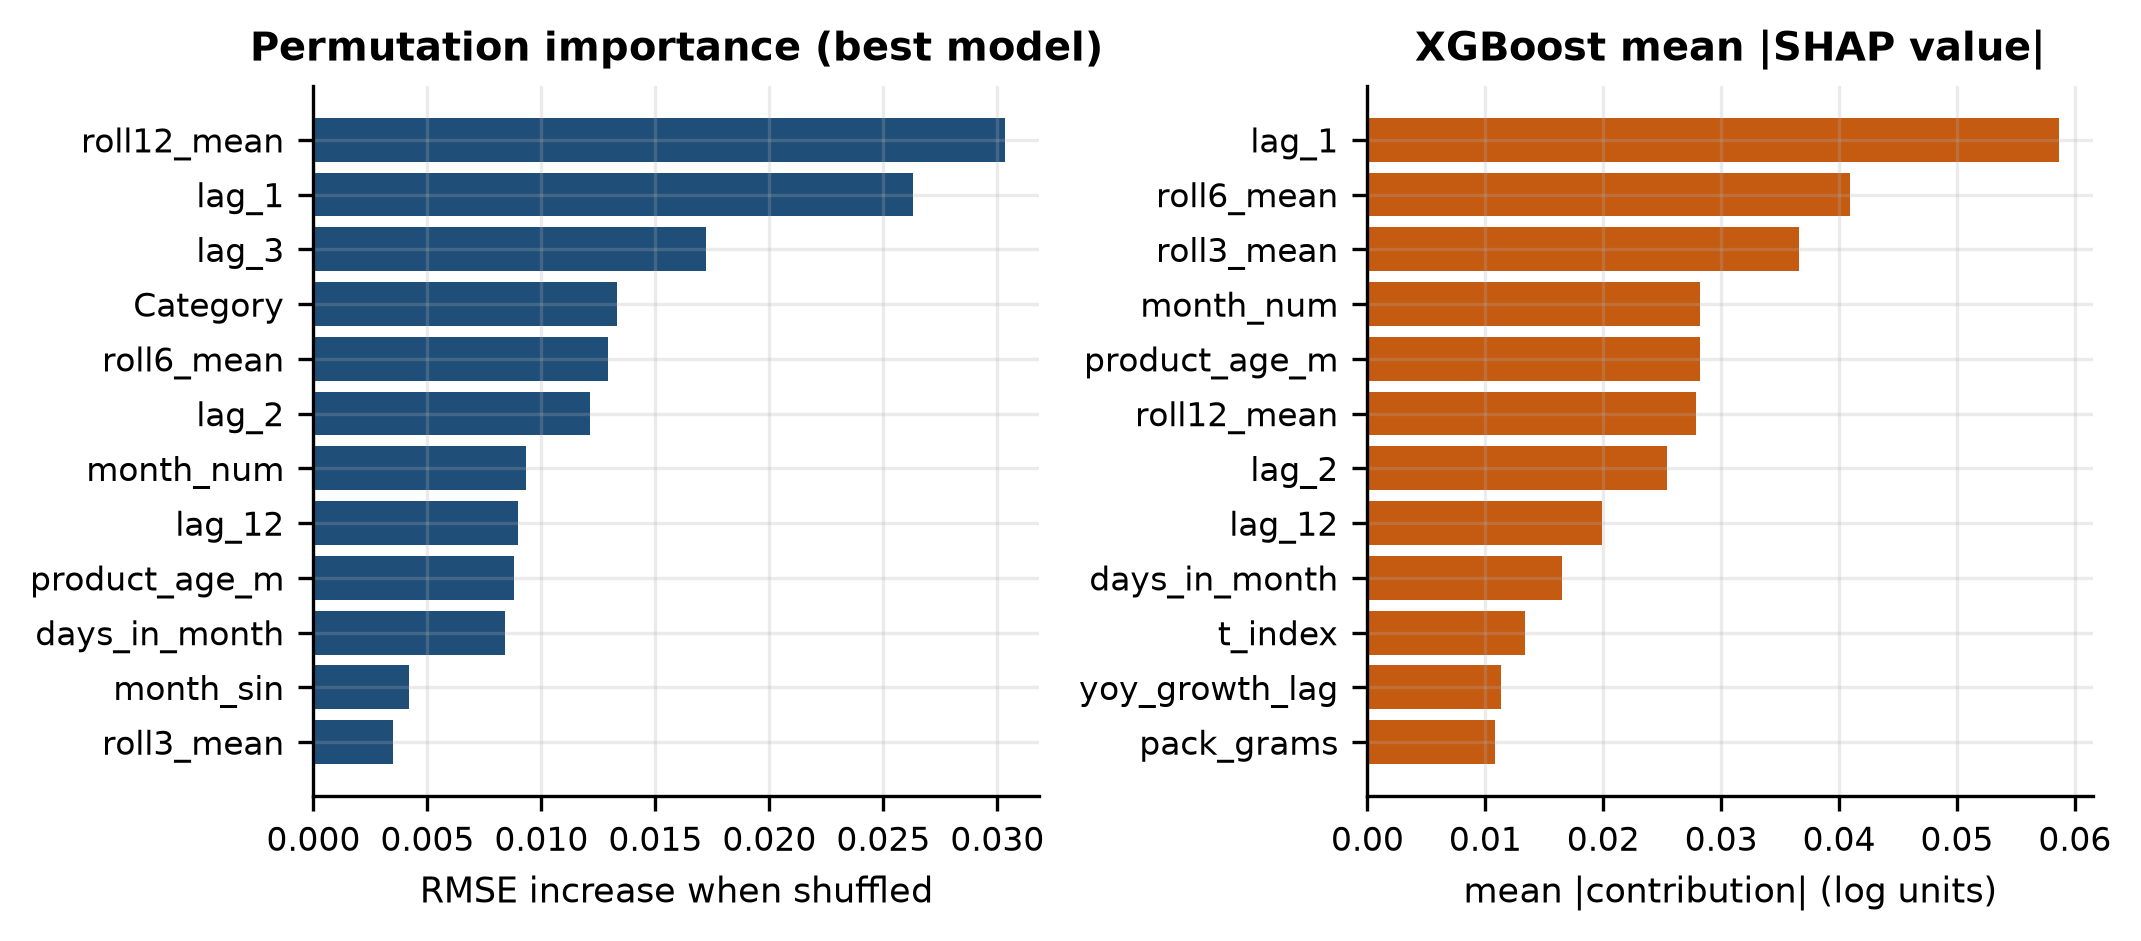
\includegraphics[width=\linewidth]{ml_feature_importance}
\caption{সেরা পূর্বাভাস মডেলের permutation importance (বামে) এবং XGBoost-এর গড় পরম SHAP মান (ডানে)}\label{fig:importance}
\end{figure}

\subsection{বারো মাসের দৃষ্টিভঙ্গি}
নির্বাচিত মডেলগুলো সেপ্টেম্বর 2026 পর্যন্ত সব ডেটায় পুনরায় প্রশিক্ষিত হয়ে অক্টোবর 2026 -- সেপ্টেম্বর 2027-এর পূর্বাভাস দিয়েছে
(\cref{tab:future}, \cref{fig:future})। এই বারো মাসে নিট বিক্রয়ের পূর্বাভাস \FutSales মিলিয়ন টাকা, 80\% ব্যবধান \FutSalesLo থেকে
\FutSalesHi মিলিয়ন, যা আগের বারো মাসের (\PrevSales মিলিয়ন টাকা) চেয়ে \FutGrowth\% বেশি। ইউনিটে পরিবর্তন প্রত্যাশিত \FutUnitsGrowth\%,
এবং ডিসেম্বরের শীর্ষ আবার ফিরবে। পূর্বাভাসে \FutTopCategory সবচেয়ে বড় ক্যাটাগরি থাকছে। এই দৃষ্টিভঙ্গি সরাসরি উৎপাদন, ক্রয় ও বাজেট
প্রক্রিয়ায় ব্যবহার করা যায়।

\begin{table}[htbp]
\centering
\footnotesize
\caption{বারো মাসের অগ্রিম পূর্বাভাস, অক্টোবর 2026 -- সেপ্টেম্বর 2027}
\label{tab:future}
\begin{adjustbox}{max width=\linewidth}
\begin{tabular}{lrrrrrrr}
\toprule
\textbf{Month} & \textbf{Units ML raw} & \textbf{Units (final)} & \textbf{80\% low} & \textbf{80\% high} & \textbf{Net sales (M)} & \textbf{80\% low } & \textbf{80\% high } \\
\midrule
Oct 2026 & 43,531 & 46,203 & 45,021 & 47,478 & 6.08 & 5.83 & 6.34 \\
Nov 2026 & 44,109 & 47,015 & 45,744 & 48,272 & 6.19 & 5.90 & 6.47 \\
Dec 2026 & 53,219 & 54,939 & 53,383 & 56,313 & 7.27 & 6.89 & 7.63 \\
Jan 2027 & 43,375 & 45,461 & 44,209 & 46,738 & 6.58 & 6.22 & 6.95 \\
Feb 2027 & 37,348 & 39,411 & 38,347 & 40,460 & 5.68 & 5.36 & 6.02 \\
Mar 2027 & 43,561 & 45,883 & 44,660 & 47,104 & 6.56 & 6.16 & 6.96 \\
Apr 2027 & 41,747 & 43,288 & 42,136 & 44,485 & 6.21 & 5.83 & 6.62 \\
May 2027 & 43,224 & 45,767 & 44,576 & 47,013 & 6.44 & 6.02 & 6.88 \\
Jun 2027 & 41,784 & 43,454 & 42,324 & 44,667 & 6.16 & 5.75 & 6.61 \\
Jul 2027 & 42,815 & 44,111 & 42,962 & 45,304 & 6.27 & 5.84 & 6.74 \\
Aug 2027 & 42,884 & 45,082 & 43,902 & 46,342 & 6.46 & 5.99 & 6.95 \\
Sep 2027 & 43,340 & 44,976 & 43,746 & 46,142 & 6.38 & 5.89 & 6.88 \\
\bottomrule
\end{tabular}
\end{adjustbox}
\par\smallskip\parbox{0.92\linewidth}{\footnotesize\emph{টীকা:} Units ML raw = reconciliation-এর আগে Random Forest পণ্য-পূর্বাভাসের যোগফল। চূড়ান্ত মোট এসেছে কোম্পানির ইউনিট ও নিট বিক্রয়ের (মিলিয়ন টাকা) Holt-Winters মডেল থেকে; ব্যবধান হলো 2,000টি সিমুলেটেড ভবিষ্যৎ-পথের 10তম ও 90তম শতাংশক। পণ্যের পূর্বাভাস এই মোটের সঙ্গে মেলানো হয়েছে।}
\end{table}

\begin{figure}[htbp]\centering
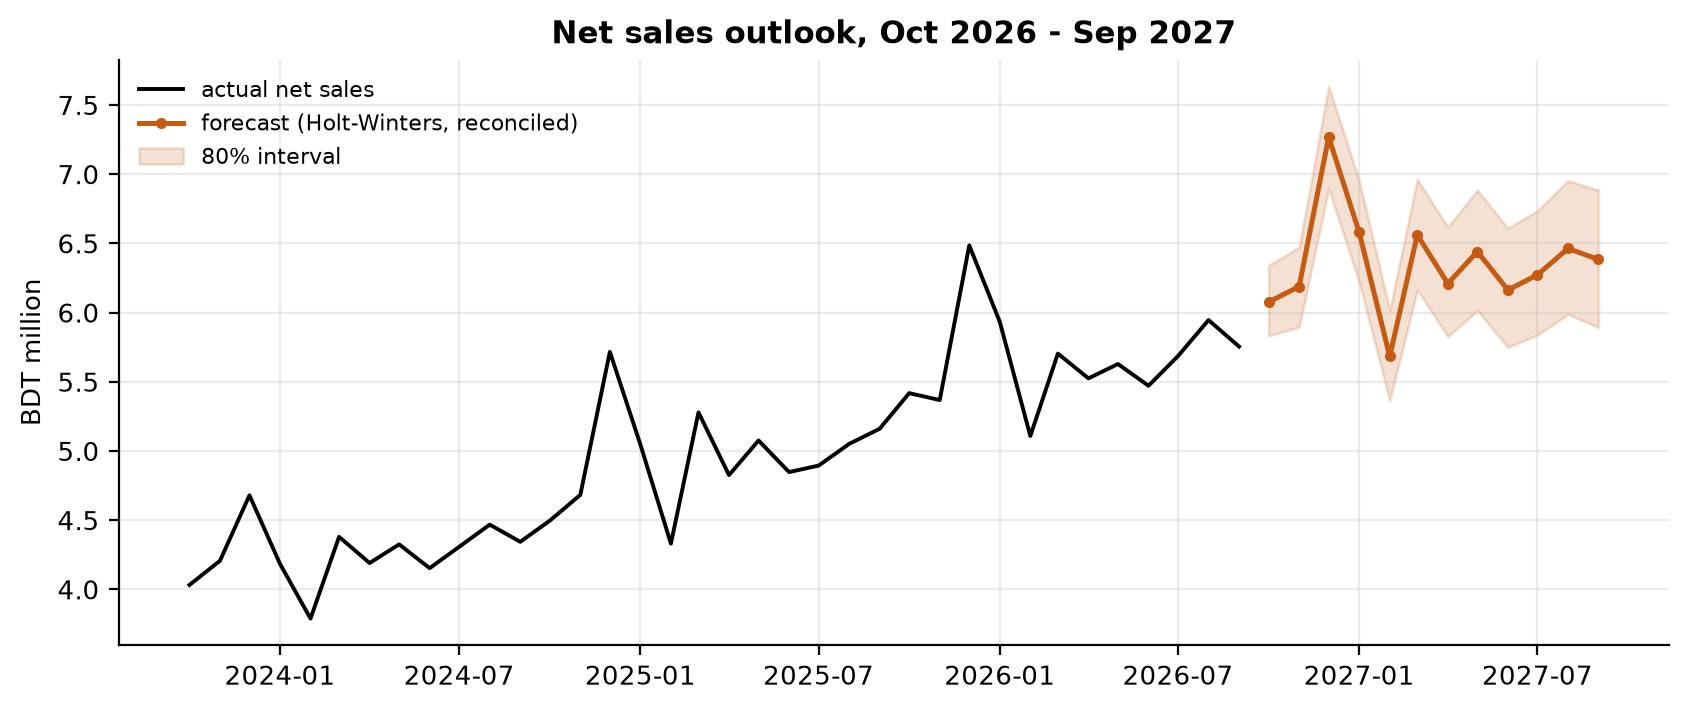
\includegraphics[width=\linewidth]{ml_future_forecast}
\caption{অক্টোবর 2026 -- সেপ্টেম্বর 2027-এর নিট বিক্রয়ের দৃষ্টিভঙ্গি, 80\% পূর্বাভাস-ব্যবধানসহ}\label{fig:future}
\end{figure}

\section{বড় অর্ডারের ক্লাসিফিকেশন}
ক্লাসিফায়ারটি অর্ডার এন্ট্রির সময় পাওয়া তথ্য থেকে অনুমান করে অর্ডারে অন্তত 10 ইউনিট থাকবে কি না। প্রশিক্ষণ-অর্ডারের \ClsPosTrain\% এবং
পরীক্ষা-অর্ডারের \ClsPosTest\% ছিল বড়। মডেলগুলো \ClsTrain টি অর্ডারে (2020--2024) প্রশিক্ষিত এবং \ClsTest টি অর্ডারে (2025--2026)
পরীক্ষিত। ফিচার: চ্যানেল, অঞ্চল, গ্রাহকের ধরন, ক্যাটাগরি, মূল্য, ডিসকাউন্ট, প্যাক সাইজ, পণ্যের বয়স ও ক্যালেন্ডার-চলক, এবং চ্যানেল
$\times$ অঞ্চল ও পণ্যের smoothed target encoding।

\begin{table}[htbp]
\centering
\footnotesize
\caption{বড় অর্ডার ক্লাসিফিকেশন ($\geq$10 ইউনিট): পরীক্ষাকালের কর্মদক্ষতা, 2025--2026}
\label{tab:classification}
\begin{adjustbox}{max width=\linewidth}
\begin{tabular}{lrrrrrrrrr}
\toprule
\textbf{Model} & \textbf{Accuracy} & \textbf{Precision} & \textbf{Recall} & \textbf{F1} & \textbf{ROC-AUC} & \textbf{PR-AUC} & \textbf{Threshold} & \textbf{Lift@10\%} & \textbf{Time (s)} \\
\midrule
Logistic Regression & 0.661 & 0.357 & 0.628 & 0.455 & 0.712 & 0.418 & 0.62 & 2.35 & 15 \\
Support Vector Machine (linear) & 0.629 & 0.341 & 0.698 & 0.458 & 0.711 & 0.417 & 0.31 & 2.34 & 42 \\
Gradient Boosting (hist) & 0.709 & 0.387 & 0.502 & 0.437 & 0.711 & 0.418 & 0.23 & 2.34 & 35 \\
Random Forest & 0.628 & 0.341 & 0.701 & 0.459 & 0.710 & 0.418 & 0.51 & 2.33 & 252 \\
XGBoost & 0.635 & 0.343 & 0.676 & 0.455 & 0.709 & 0.416 & 0.20 & 2.34 & 60 \\
Decision Tree & 0.550 & 0.309 & 0.807 & 0.447 & 0.709 & 0.407 & 0.48 & 2.31 & 14 \\
K-Nearest Neighbors & 0.634 & 0.333 & 0.624 & 0.434 & 0.684 & 0.396 & 0.20 & 2.28 & 73 \\
\bottomrule
\end{tabular}
\end{adjustbox}
\par\smallskip\parbox{0.92\linewidth}{\footnotesize\emph{টীকা:} পরীক্ষা-বছরে বড় অর্ডারের হার: 22.5\%; যে ক্লাসিফায়ার সবসময় `বড় নয়' বলে তার accuracy হতো 77.5\%, তাই কেবল accuracy বিভ্রান্তিকর। Threshold 2024 validation-বছরে F1 সর্বোচ্চ করে। KNN 60,000-সারির প্রশিক্ষণ-নমুনা ব্যবহার করে। Lift@10\% = সর্বোচ্চ স্কোরের 10\% অর্ডারে বড় অর্ডারের হার ভাগ সামগ্রিক হার।}
\end{table}

\Cref{tab:classification} ও \cref{fig:classification} একটি স্পষ্ট ও শিক্ষণীয় ফলাফল দেখায়। সাতটি অ্যালগরিদমেরই ROC-AUC প্রায় সমান,
\ClsAUCmin থেকে \ClsAUC, এবং \ClsBest সেরা। যে মডেল সবসময় ``বড় নয়'' বলে, সেটি \ClsMajority\% নির্ভুল হলেও অকেজো। বিপরীতে টিউন
করা মডেলগুলো বেশিরভাগ বড় অর্ডার খুঁজে পায় (\ClsBest-এর recall প্রায় \ClsRecall) মাঝারি precision-এ, এবং স্কোর অনুযায়ী শীর্ষ 10\%
অর্ডারে বড় অর্ডার গড়ের চেয়ে \ClsLift গুণ বেশি। সীমা নির্ধারণ করছে ডেটায় থাকা \emph{তথ্য}, অ্যালগরিদম নয়: XGBoost (\ClsXGBAUC)
logistic regression-এর চেয়ে কিছুই বাড়ায় না, আর KNN (\ClsKNNAUC) সবচেয়ে দুর্বল, কারণ অনেক one-hot ফিচারে দূরত্ব অর্থহীন হয়ে পড়ে।

\begin{figure}[htbp]\centering
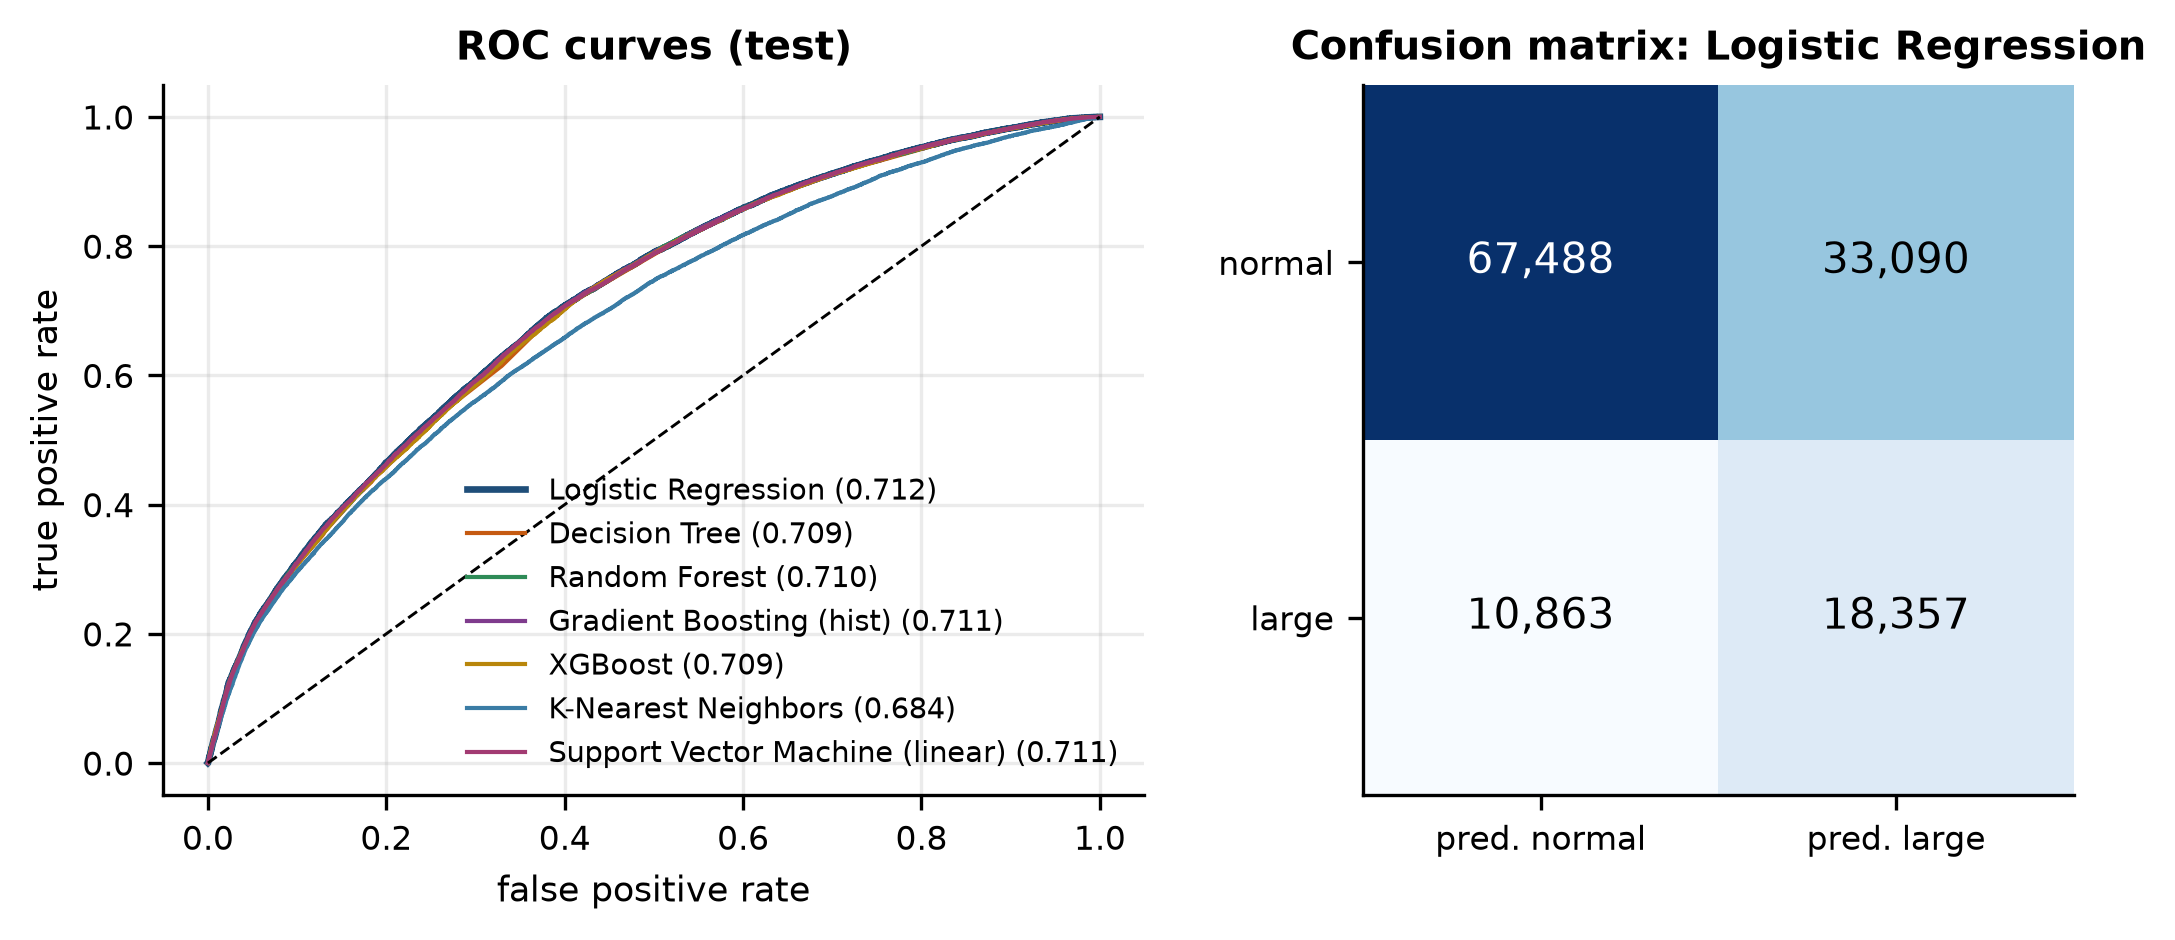
\includegraphics[width=\linewidth]{ml_classification}
\caption{বড় অর্ডার ক্লাসিফিকেশনের ROC বক্ররেখা (বামে), সেরা মডেলের confusion matrix (মাঝে) এবং মেট্রিক তুলনা (ডানে)}\label{fig:classification}
\end{figure}

XGBoost-এর gain importance (\cref{fig:clsimp}) কারণটি চিহ্নিত করে: মডেলের gain-এর প্রায় \ClsChannelImp\% আসে বিক্রয় চ্যানেল থেকে
এবং প্রায় \ClsRegionImp\% অঞ্চল থেকে, আর পণ্য, মূল্য, ডিসকাউন্ট ও ক্যালেন্ডারের অবদান অতি সামান্য। পরীক্ষা-বছরগুলোতে ডিস্ট্রিবিউটর
অর্ডারের \LargeDist\% ছিল বড়, অথচ E-commerce অর্ডারের মাত্র \LargeEcom\%। চ্যানেল ও অঞ্চলের ভেতরে অর্ডারের আকার প্রায় এলোমেলো।
তাই সিদ্ধান্ত গ্রহণে উপযোগী ফল হলো লজিস্টিক পরিকল্পনার জন্য \emph{চ্যানেল-ও-অঞ্চল-স্তরের} বড় অর্ডারের প্রত্যাশা, অর্ডার-বাই-অর্ডার
সুনির্দিষ্ট পূর্বাভাস নয়।

\begin{figure}[htbp]\centering
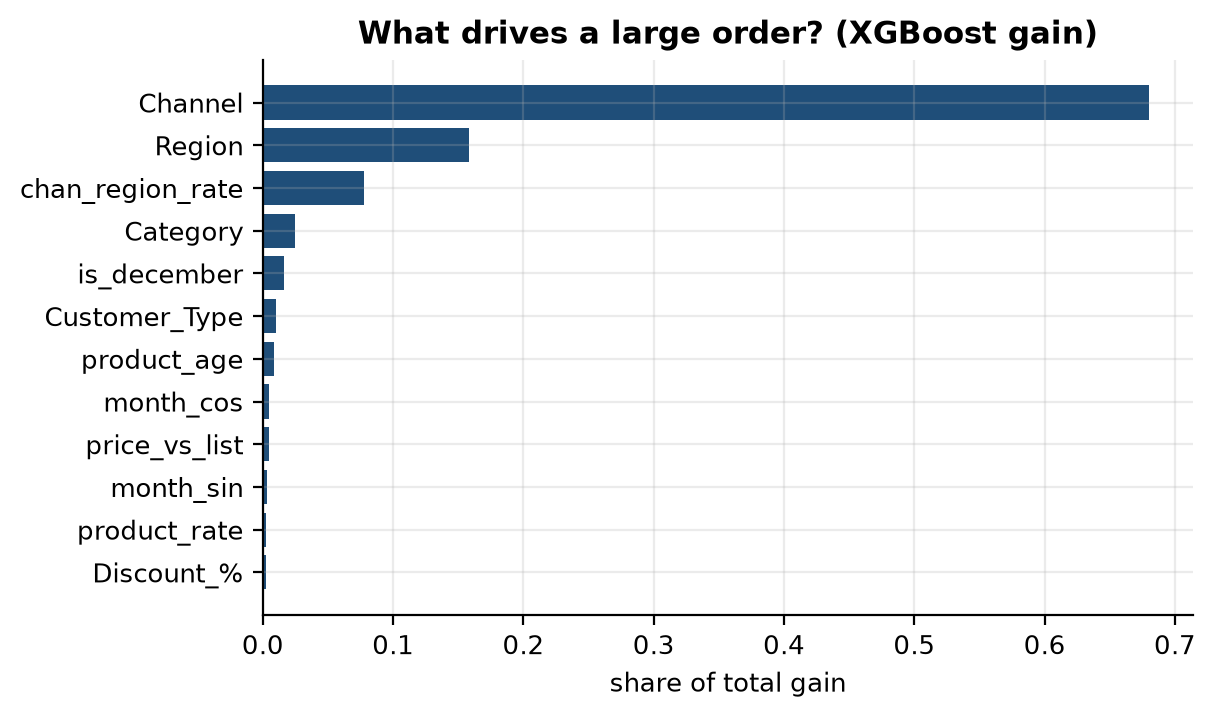
\includegraphics[width=.65\linewidth]{ml_classification_importance}
\caption{বড় অর্ডারের চালিকাশক্তি: মূল চলক অনুযায়ী একত্রিত XGBoost gain}\label{fig:clsimp}
\end{figure}

\section{বিভাজন}
\subsection{পণ্য পোর্টফোলিও}
প্রতিটি পণ্যকে বর্ণনা করা হয়েছে এর log আয়, log গড় মূল্য, 2023 থেকে 2025-এর ইউনিট প্রবৃদ্ধি, ডিসেম্বর মৌসুমি সূচক এবং মাস-থেকে-মাসের
অস্থিরতা দিয়ে। অর্ডারের আকার ও চ্যানেল-মিশ্রণ বাদ দেওয়া হয়েছে, কারণ পণ্যভেদে এগুলো প্রায় একই (\cref{ch:eda}) এবং কেবল noise যোগ
করত। ফিচারগুলো standardise করে $k=2,\dots,8$-এর জন্য $K$-Means, agglomerative (Ward) ও Gaussian-mixture ক্লাস্টারিং তুলনা করা হয়েছে
(\cref{fig:clustering}, \cref{tab:clustercompare})। তিন থেকে পাঁচটি বিভাগের ব্যবহারিক সীমার মধ্যে $k=\ProdK$-এ $K$-Means সেরা silhouette
(\ProdSil) ও Davies--Bouldin সূচক \ProdDB দিয়েছে। ফলস্বরূপ বিভাগগুলো \cref{tab:productclusters}-এ সংক্ষেপিত এবং তাদের গড় থেকে
স্বয়ংক্রিয়ভাবে নামকরণ করা।

\begin{table}[htbp]
\centering
\small
\caption{পণ্য-পোর্টফোলিওর বিভাগ (K-Means, k=5)}
\label{tab:productclusters}
\begin{adjustbox}{max width=\linewidth}
\begin{tabular}{lrrrrrr}
\toprule
\textbf{Segment} & \textbf{Products} & \textbf{Sales share \%} & \textbf{Avg price} & \textbf{Units/order} & \textbf{Unit growth \%/yr} & \textbf{Dec. index} \\
\midrule
Premium \& gift packs & 13 & 33.3 & 156 & 6.24 & +7.8 & 123 \\
Mature slow-growth lines & 13 & 31.9 & 130 & 6.17 & +2.3 & 120 \\
Core family packs & 11 & 28.1 & 133 & 6.17 & +4.9 & 134 \\
Single-serve value packs & 9 & 4.2 & 23 & 6.22 & +6.0 & 119 \\
Niche \& new lines & 6 & 2.5 & 24 & 6.22 & +4.0 & 134 \\
\bottomrule
\end{tabular}
\end{adjustbox}
\par\smallskip\parbox{0.92\linewidth}{\footnotesize\emph{টীকা:} প্রবৃদ্ধি হলো 2023 থেকে 2025-এর মধ্যে ইউনিটের চক্রবৃদ্ধি বার্ষিক হার। ডিসেম্বর সূচক = পণ্যের গড় মাসের তুলনায় গড় ডিসেম্বরের ইউনিট (100 = মৌসুমিতা নেই)।}
\end{table}

\subsection{বাজার-বিভাগ}
অঞ্চল, চ্যানেল ও গ্রাহকের ধরনের 220টি সমন্বয়কে তাদের আয়, গড় অর্ডার-মূল্য, অর্ডারপ্রতি ইউনিট, মূল্য, ডিসকাউন্ট, প্রবৃদ্ধি ও গিফট-প্যাকের
অংশ দিয়ে ক্লাস্টার করা হয়েছে। $K$-Means $k=\MktK$টি বিভাগ বেছে নিয়েছে (silhouette \MktSil), যা স্পষ্টভাবে ভাগ হয়: \emph{core retail
trade} (বড় শহরে General ও Modern Trade), \emph{bulk distribution}, ছোট-অঙ্কের \emph{online ও আঞ্চলিক} কোষ, এবং একদল
\emph{উদীয়মান উচ্চ-প্রবৃদ্ধির} কোষ (\cref{tab:marketclusters})।

\begin{table}[htbp]
\centering
\scriptsize
\caption{অঞ্চল $\times$ চ্যানেল $\times$ গ্রাহকের ধরন কোষের বাজার-বিভাগ (K-Means, k=4)}
\label{tab:marketclusters}
\begin{adjustbox}{max width=\linewidth}
\begin{tabular}{lrrrrrll}
\toprule
\textbf{Segment} & \textbf{Cells} & \textbf{Sales share \%} & \textbf{AOV (BDT)} & \textbf{Units/order} & \textbf{Growth \%/yr} & \textbf{Main channels} & \textbf{Main regions} \\
\midrule
Core retail trade & 99 & 71.9 & 518 & 5.02 & +14.8 & General Trade, Modern Trade & Dhaka, Chattogram, Gazipur \\
Bulk distribution & 52 & 22.6 & 966 & 9.96 & +16.2 & Distributor & Chattogram, Dhaka, Gazipur \\
Small-ticket online \& regional & 50 & 4.2 & 341 & 3.43 & +16.7 & E-commerce, Modern Trade & Barishal, Khulna, Rajshahi \\
Emerging high-growth cells & 19 & 1.3 & 431 & 4.16 & +33.2 & E-commerce, Modern Trade & Cumilla, Khulna, Mymensingh \\
\bottomrule
\end{tabular}
\end{adjustbox}
\end{table}
\begin{table}[htbp]
\centering
\small
\caption{নির্বাচিত ক্লাস্টার-সংখ্যায় ক্লাস্টারিং অ্যালগরিদমগুলোর তুলনা}
\label{tab:clustercompare}
\begin{adjustbox}{max width=\linewidth}
\begin{tabular}{llrrrr}
\toprule
\textbf{Problem} & \textbf{Algorithm} & \textbf{k} & \textbf{Silhouette} & \textbf{Davies-Bouldin} & \textbf{Calinski-Harabasz} \\
\midrule
Products & K-Means & 5 & 0.237 & 1.271 & 16.2 \\
Products & Agglomerative (Ward) & 5 & 0.212 & 1.195 & 14.9 \\
Products & Gaussian Mixture & 5 & 0.233 & 1.237 & 15.3 \\
Market cells & K-Means & 4 & 0.243 & 1.497 & 54.2 \\
Market cells & Agglomerative (Ward) & 4 & 0.250 & 1.467 & 48.9 \\
Market cells & Gaussian Mixture & 4 & 0.165 & 1.753 & 42.4 \\
\bottomrule
\end{tabular}
\end{adjustbox}
\par\smallskip\parbox{0.92\linewidth}{\footnotesize\emph{টীকা:} উচ্চতর silhouette ও Calinski--Harabasz এবং নিম্নতর Davies--Bouldin মান বেশি পৃথক ক্লাস্টার নির্দেশ করে।}
\end{table}

\begin{figure}[htbp]\centering
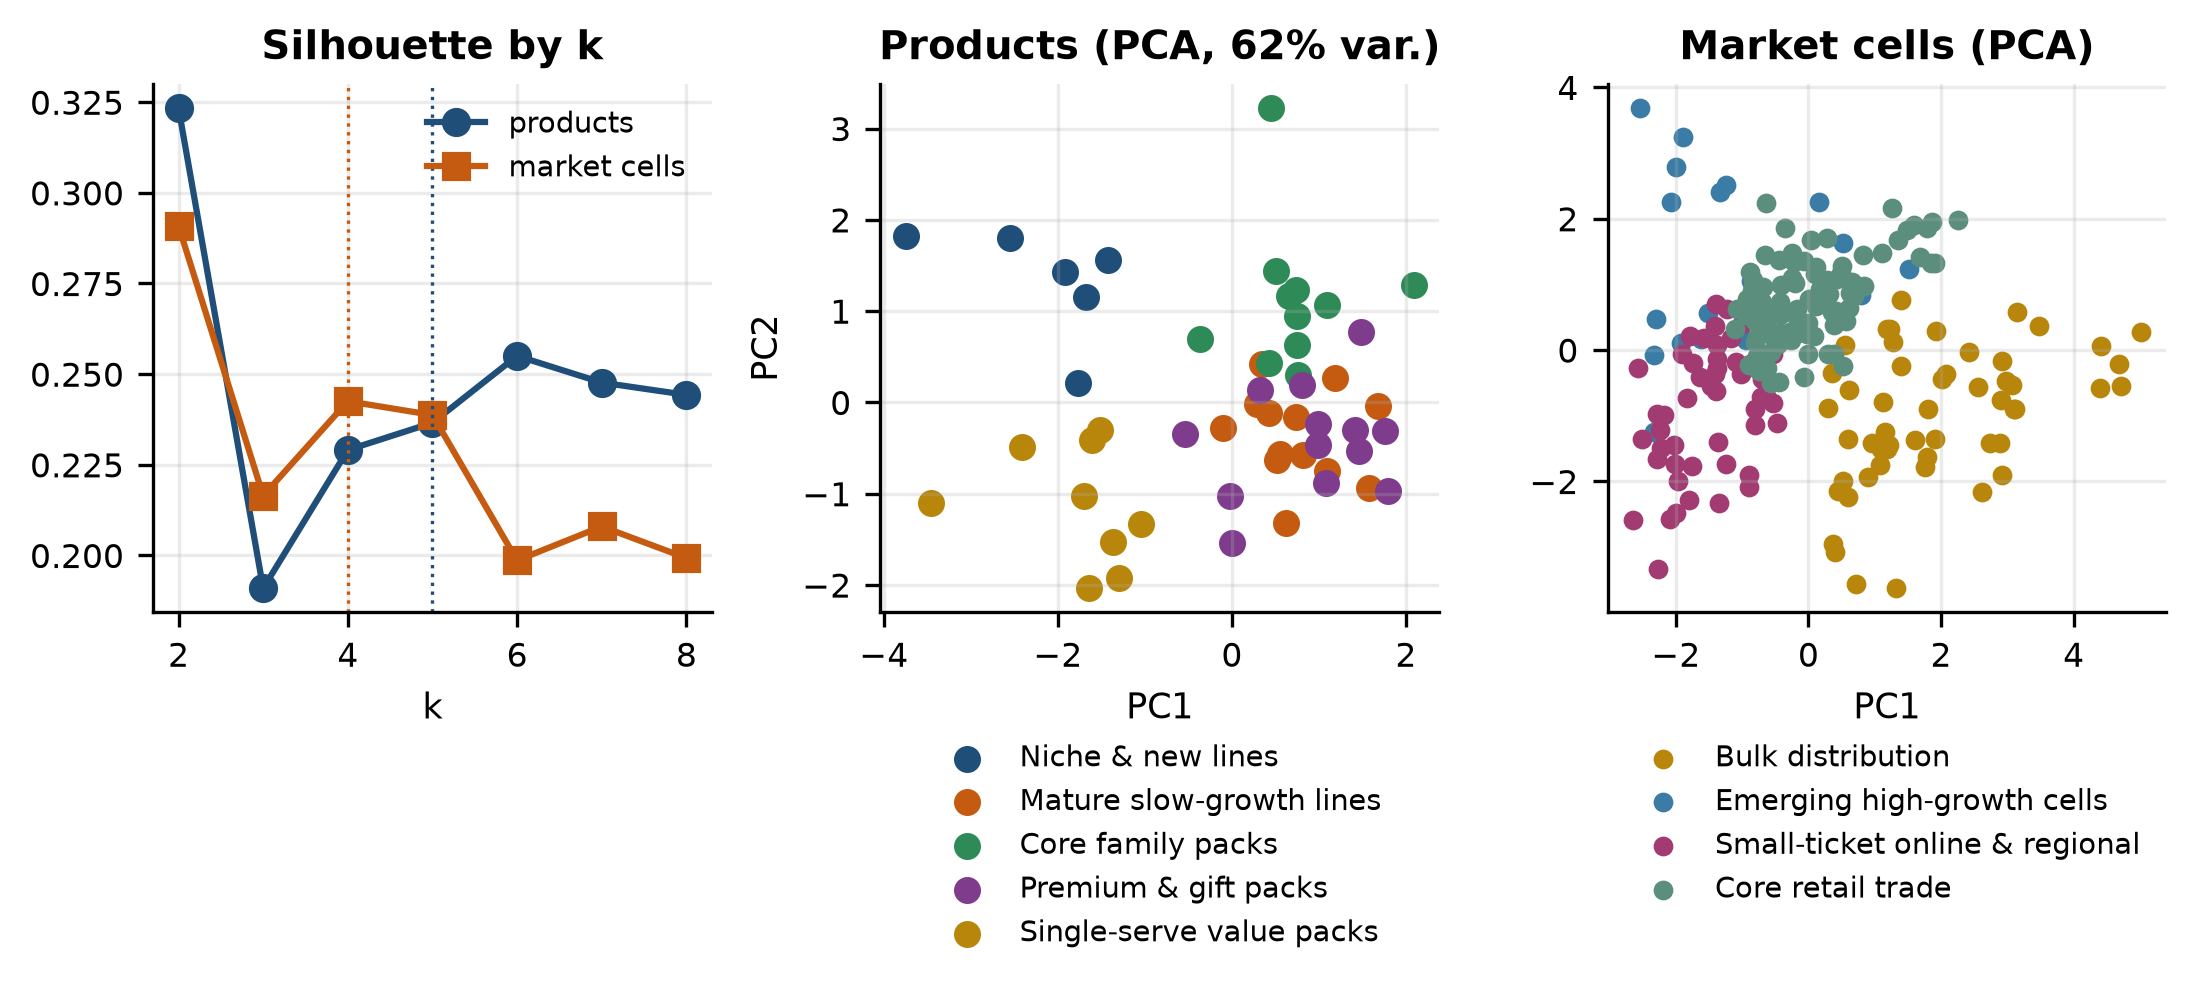
\includegraphics[width=\linewidth]{ml_clustering}
\caption{ক্লাস্টারের সংখ্যা অনুযায়ী silhouette স্কোর (বামে); প্রথম দুটি principal component-এ প্রক্ষিপ্ত পণ্য (মাঝে) ও বাজার-কোষ (ডানে)}\label{fig:clustering}
\end{figure}

Silhouette মান (\ProdSil ও \MktSil) দুর্বল থেকে মাঝারি কাঠামো নির্দেশ করে \citep{rousseeuw1987}। তাই বিভাগগুলো কৌশলের জন্য উপযোগী
সারসংক্ষেপ, স্পষ্টভাবে পৃথক প্রাকৃতিক দল নয়। $K$-Means ও Ward ক্লাস্টারিং প্রায় একমত ছিল, আর এই ছোট নমুনায় Gaussian mixture
সবচেয়ে দুর্বল। পাঠক যাতে বিভাজনের দৃঢ়তা বিচার করতে পারেন, সে জন্য এই ক্রম উল্লেখ করা হলো।

\section{অ্যানোমালি ডিটেকশন}
\subsection{দৈনিক পর্যবেক্ষণ}
প্রতিটি দিনের প্রত্যাশিত মান হিসাব করা হয়েছে একটি 31-দিনের কেন্দ্রীভূত rolling median-কে বছরের মাস অনুযায়ী মৌসুমি গুণক দিয়ে গুণ করে।
বিচ্যুতিগুলো log স্কেলে robust $z$-score $z = 0.6745\,(r-\tilde r)/\text{MAD}$ দিয়ে এবং আলাদাভাবে চারটি দৈনিক ফিচারের উপর একটি
Isolation Forest দিয়ে স্কোর করা হয়েছে। দুটি পদ্ধতি মিলে 2,465টি ব্যবসায়িক দিনের মধ্যে \AnomDays টি চিহ্নিত করেছে: robust $z$-score
দিয়ে \AnomDaysZ টি ও Isolation Forest দিয়ে \AnomDaysIF টি (\cref{fig:anomdaily}, \cref{tab:dailyanom})। বেশিরভাগ চিহ্নিত দিন অস্বাভাবিক
দুর্বল ব্যবসায়িক দিন; বাস্তব প্রয়োগে প্রতিটি দিন সরকারি ছুটি, ধর্মঘট বা সিস্টেম-বিভ্রাটের মতো জানা কারণের সঙ্গে মিলিয়ে দেখা হবে।

\begin{figure}[htbp]\centering
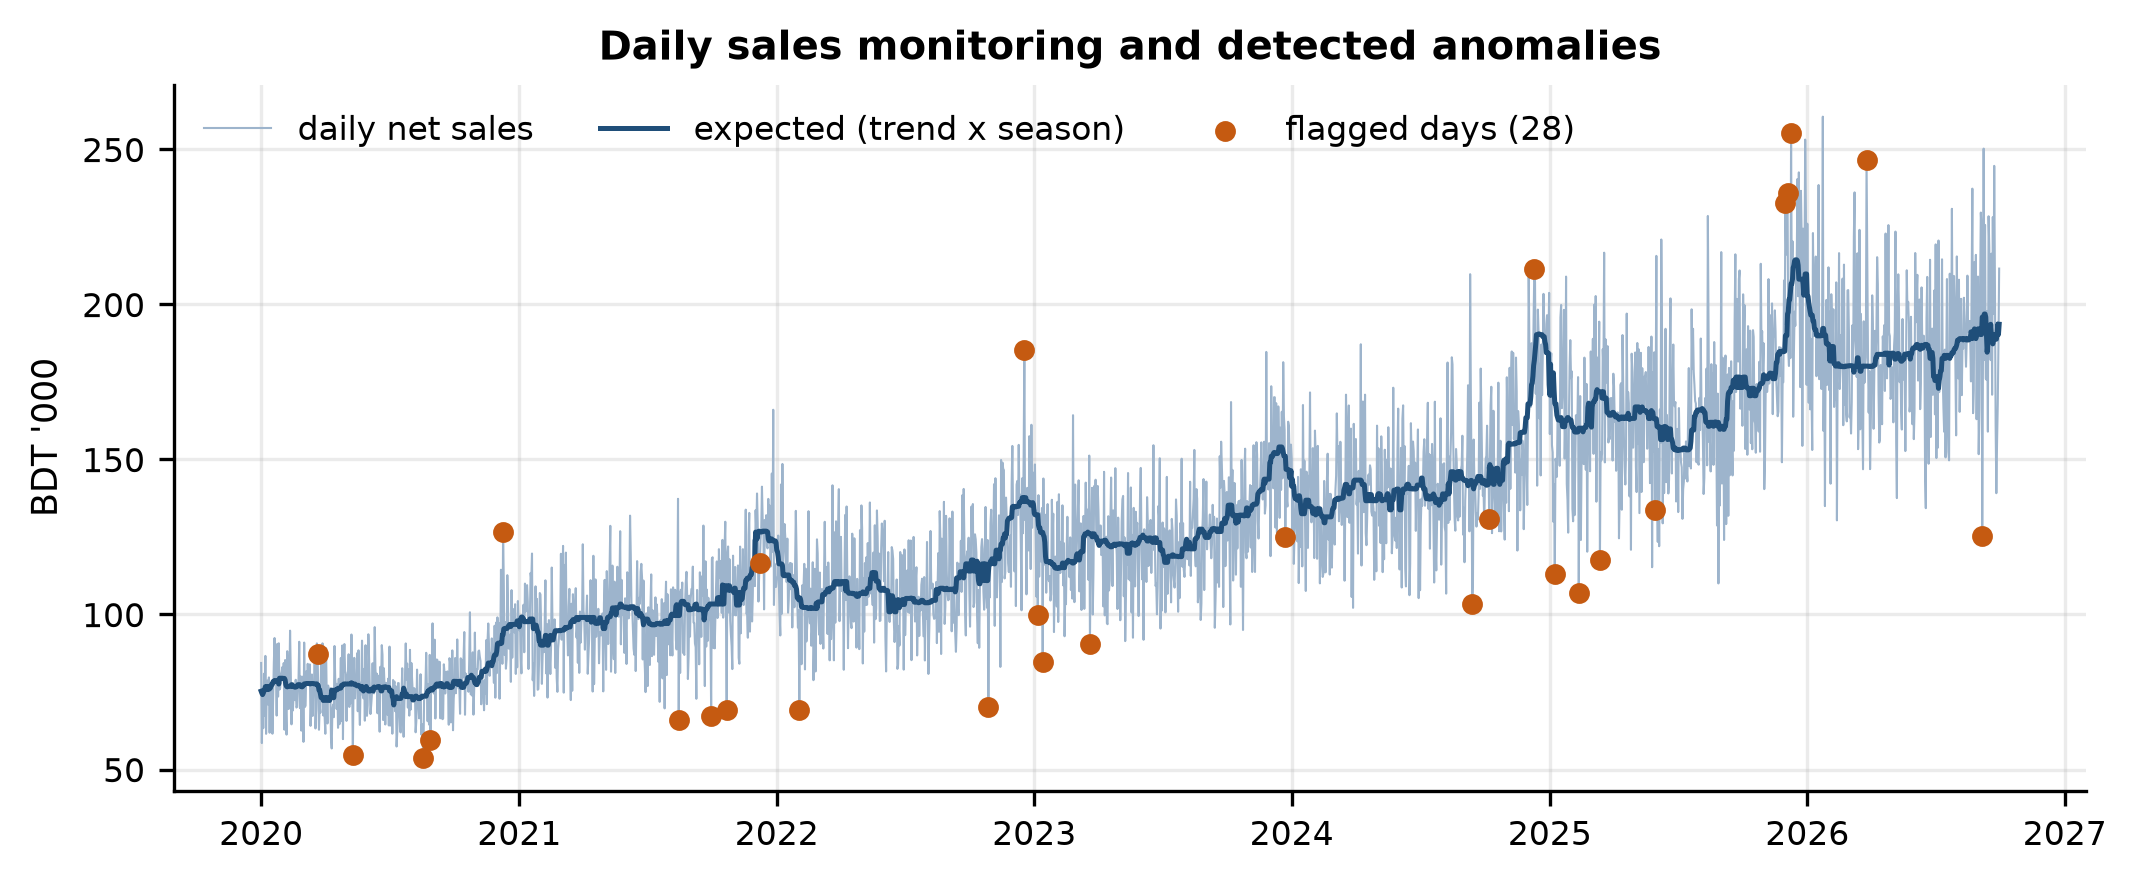
\includegraphics[width=\linewidth]{anomaly_daily}
\caption{দৈনিক নিট বিক্রয়, প্রত্যাশিত স্তর ও শনাক্তকৃত অস্বাভাবিকতা}\label{fig:anomdaily}
\end{figure}
\begin{table}[htbp]
\centering
\small
\caption{দশটি সবচেয়ে অস্বাভাবিক ব্যবসায়িক দিন (মৌসুমি-সমন্বিত)}
\label{tab:dailyanom}
\begin{adjustbox}{max width=\linewidth}
\begin{tabular}{lrrrrl}
\toprule
\textbf{Date} & \textbf{Net sales (BDT)} & \textbf{Expected (BDT)} & \textbf{Deviation \%} & \textbf{Robust z} & \textbf{Flagged by} \\
\midrule
28 Oct 2022 & 70,215 & 113,462 & -38.1 & -4.01 & robust z \\
22 Oct 2021 & 69,194 & 109,276 & -36.7 & -3.82 & robust z \\
06 Sep 2026 & 125,262 & 195,913 & -36.1 & -3.74 & robust z \\
30 Sep 2021 & 67,358 & 103,385 & -34.8 & -3.58 & both \\
02 Feb 2022 & 69,149 & 104,763 & -34.0 & -3.47 & Isolation Forest \\
15 Aug 2021 & 66,039 & 99,664 & -33.7 & -3.44 & Isolation Forest \\
11 Feb 2025 & 106,843 & 160,093 & -33.3 & -3.38 & Isolation Forest \\
13 Jan 2023 & 84,814 & 126,483 & -32.9 & -3.34 & Isolation Forest \\
08 Jan 2025 & 113,188 & 168,043 & -32.6 & -3.31 & Isolation Forest \\
13 Mar 2025 & 117,699 & 171,855 & -31.5 & -3.17 & Isolation Forest \\
\bottomrule
\end{tabular}
\end{adjustbox}
\end{table}

\subsection{লেনদেন যাচাই}
লেবেলযুক্ত ত্রুটি না থাকায় প্রকৃত ডেটায় ডিটেক্টরের সক্ষমতা মাপা যায় না। তাই প্রিপ্রসেসিং স্ক্রিপ্টের পদ্ধতি অনুসরণ করে 500,000 অর্ডারের
একটি অনুলিপিতে চার ধরনের (প্রতিটি 250টি) মোট 1,000টি বাস্তবসম্মত ত্রুটি রোপণ করা হয়েছে (\cref{tab:anomaly})। পরিমাণের উপর প্রতি-পণ্য
IQR নিয়ম রোপিত ত্রুটির মাত্র \AnomIQRRecall\% ধরেছে, কারণ চার ধরনের তিনটিতে পরিমাণ জড়িত নয়। মূল্য ও ডিসকাউন্টের উপর সরল ব্যবসায়িক
নিয়ম নিখুঁত precision-এ \AnomRuleRecall\% ধরেছে, কিন্তু পরিমাণের সব ত্রুটি বাদ পড়েছে। Isolation Forest চার ধরনেই মিলিয়ে \AnomIFRecall\%
ধরেছে: মূল্য ও ডিসকাউন্টের ত্রুটি সম্পূর্ণভাবে, এবং বেশিরভাগ স্ফীত পরিমাণও। শিক্ষা হলো নিয়ম ও মেশিন লার্নিং পরস্পরের পরিপূরক: জানা
ব্যর্থতার ক্ষেত্রে নিয়ম নিখুঁত, আর অজানা ক্ষেত্রে Isolation Forest বিস্তৃত সুরক্ষা দেয়।

\begin{table}[htbp]
\centering
\footnotesize
\caption{500,000 অর্ডারে রোপিত 1,000টি লেনদেন-ত্রুটির শনাক্তকরণ}
\label{tab:anomaly}
\begin{adjustbox}{max width=\linewidth}
\begin{tabular}{lrrrrrrr}
\toprule
\textbf{Method} & \textbf{Flagged} & \textbf{Precision} & \textbf{Recall} & \textbf{Price x10} & \textbf{Qty x20} & \textbf{Disc. 30-45\%} & \textbf{Price 10\%} \\
\midrule
IQR on log quantity (per product) & 1,500 & 0.112 & 0.168 & 0.00 & 0.66 & 0.00 & 0.01 \\
Business rules (price, discount) & 750 & 1.000 & 0.750 & 1.00 & 0.00 & 1.00 & 1.00 \\
Isolation Forest (4 features) & 2,500 & 0.364 & 0.909 & 1.00 & 0.64 & 1.00 & 1.00 \\
Rules OR Isolation Forest & 2,500 & 0.364 & 0.909 & 1.00 & 0.64 & 1.00 & 1.00 \\
\bottomrule
\end{tabular}
\end{adjustbox}
\par\smallskip\parbox{0.92\linewidth}{\footnotesize\emph{টীকা:} শেষ চারটি কলাম দেখায় প্রতিটি ধরনের ত্রুটির কত অংশ শনাক্ত হয়েছে। ডেটার একটি অনুলিপিতে প্রতিটি ধরনের 250টি ত্রুটি রোপণ করা হয়েছে।}
\end{table}

\section{মডেল মূল্যায়নের সারসংক্ষেপ}
\begin{table}[htbp]\centering\small
\caption{প্রতিটি বিশ্লেষণী সমস্যার জন্য নির্বাচিত মডেলের সারসংক্ষেপ}\label{tab:modelsummary}
\begin{tabularx}{\linewidth}{@{}lXl@{}}
\toprule
\textbf{সমস্যা} & \textbf{নির্বাচিত পদ্ধতি} & \textbf{প্রধান পরীক্ষা-ফল} \\ \midrule
পণ্যের চাহিদা (এক-ধাপ) & \BestReg & WAPE \BestRegWAPE\%, $R^2$ \BestRegRtwo \\
পণ্যের চাহিদা (বহু-ধাপ) & \BestRec, recursive & WAPE \BestRecWAPE\% \\
কোম্পানির মোট & Holt--Winters + top-down reconciliation & MAPE \HWMAPE\% \\
বড় অর্ডার & \ClsBest & ROC-AUC \ClsAUC, lift \ClsLift \\
পণ্য-বিভাগ & $K$-Means, $k=\ProdK$ & silhouette \ProdSil \\
বাজার-বিভাগ & $K$-Means, $k=\MktK$ & silhouette \MktSil \\
লেনদেনের অস্বাভাবিকতা & নিয়ম অথবা Isolation Forest & recall \AnomComboRecall\% \\ \bottomrule
\end{tabularx}
\end{table}
প্রস্তাবনার নির্দেশ অনুযায়ী মডেল বাছাই করা হয়েছে উপযুক্ত মেট্রিক \emph{এবং} ব্যবসায়িক প্রাসঙ্গিকতা দিয়ে, কেবল নির্ভুলতা দিয়ে নয়। যেখানে
সরল মডেল জটিল মডেলের সমান কাজ করেছে (যেমন ক্লাসিফিকেশনে logistic regression বনাম XGBoost), সেখানে সরল ও বেশি ব্যাখ্যাযোগ্য মডেলটি
অগ্রাধিকার পেয়েছে।

\chapter[বিজনেস ইন্টেলিজেন্স ড্যাশবোর্ড ও সিদ্ধান্ত-সহায়তা]{বিজনেস ইন্টেলিজেন্স ড্যাশবোর্ড ও\\ সিদ্ধান্ত-সহায়তা}\label{ch:dashboard}

\section{নকশার লক্ষ্য}
ড্যাশবোর্ড হলো সেই জায়গা যেখানে কাঠামোটি এর ব্যবহারকারী, অর্থাৎ বিক্রয়, সাপ্লাই-চেইন ও ঊর্ধ্বতন ব্যবস্থাপকদের সঙ্গে মিলিত হয়।
\citet{few2013} অনুসরণ করে এটি পাঁচটি প্রয়োজন পূরণের জন্য নকশা করা হয়েছে:
\begin{enumerate}
  \item \textbf{এক নজরে KPI}: ওভারভিউ পাতার শীর্ষে নিট বিক্রয়, ইউনিট, অর্ডার, গড় অর্ডার-মূল্য, ডিসকাউন্ট হার ও বছরের-শুরু-থেকে প্রবৃদ্ধি;
  \item \textbf{সামঞ্জস্যপূর্ণ ফিল্টার}: এক সেট ফিল্টার (বছর, অঞ্চল, চ্যানেল, গ্রাহকের ধরন, ক্যাটাগরি) সব পাতায় প্রযোজ্য;
  \item \textbf{তিনটি ব্যবস্থাপনা প্রশ্ন}: পাতাগুলো \emph{কী ঘটেছে} (ওভারভিউ, প্রবণতা, পণ্য, বাজার) থেকে \emph{কেন} (চালিকাশক্তি,
        বিভাগ) এবং \emph{সামনে কী} (পূর্বাভাস, অস্বাভাবিকতা, সুপারিশ) পর্যন্ত এগোয়;
  \item \textbf{সৎ উপস্থাপন}: পূর্বাভাস সবসময় পূর্বাভাস-ব্যবধানসহ দেখানো হয়, মডেলের নির্ভুলতা ব্যবহারকারীর কাছে দৃশ্যমান, এবং রং কেবল
        অর্থ বোঝাতে ব্যবহৃত;
  \item \textbf{বিনামূল্যে ও সহজলভ্য}: ড্যাশবোর্ড যেকোনো ওয়েব ব্রাউজারে চলে এবং বিনা খরচে হোস্ট করা হয়।
\end{enumerate}

\section{বাস্তবায়ন}
ড্যাশবোর্ডটি Streamlit ও Plotly দিয়ে একটি একক Python ফাইলে (\path{dashboard/app.py}) তৈরি। এটি 500,000টি কাঁচা সারি পড়ে না, বরং
পাইপলাইনের তৈরি সংক্ষিপ্ত সমষ্টিগত ডেটা পড়ে: অঞ্চল $\times$ চ্যানেল $\times$ গ্রাহকের ধরন $\times$ ক্যাটাগরি অনুযায়ী একটি মাসিক
কিউব, পণ্য-বাই-অঞ্চল মাসিক মোট, পূর্বাভাস, মডেল-স্কোর, বিভাগ-সারণি ও অস্বাভাবিকতার তালিকা। এদের মোট আকার প্রায় 2~MB, তাই বিনামূল্যের
হোস্টিংয়ে অ্যাপটি কয়েক সেকেন্ডে চালু হয়, অথচ প্রতিটি ফিল্টার-সমন্বয় নির্ভুল থাকে। প্রথমবার লোডের পর ডেটা মেমোরিতে cache থাকে।
\Cref{tab:pages}-এ নয়টি পাতার তালিকা।

\begin{table}[htbp]\centering\small
\caption{ইন্টারঅ্যাকটিভ ড্যাশবোর্ডের পাতাসমূহ}\label{tab:pages}
\begin{tabularx}{\linewidth}{@{}lX@{}}
\toprule
\textbf{পাতা} & \textbf{বিষয়বস্তু} \\ \midrule
Executive overview & KPI কার্ড, চলমান গড়সহ মাসিক বিক্রয়, ক্যাটাগরি, অঞ্চল ও চ্যানেলের মিশ্রণ, বার্ষিক সারণি \\
Trends \& seasonality & যেকোনো মাত্রায় স্তূপীকৃত প্রবণতা, বছর $\times$ মাস heat map, মৌসুমি সূচক, বছর-বনাম-বছর রেখা \\
Products \& portfolio & শীর্ষ-$N$ পণ্য, Pareto/ABC বিশ্লেষণ, ML পণ্য-বিভাগ, একক পণ্যের বিস্তারিত \\
Markets \& customers & অঞ্চল $\times$ চ্যানেল heat map, গ্রাহকের ধরন, আঞ্চলিক CAGR, ML বাজার-বিভাগ \\
Demand forecast & ব্যবধানসহ 12-মাসের দৃষ্টিভঙ্গি, ক্যাটাগরি ও পণ্যের পূর্বাভাস, মডেল লিডারবোর্ড, CSV ডাউনলোড \\
Machine-learning models & feature importance-সহ রিগ্রেশন, ক্লাসিফিকেশন ও ক্লাস্টারিংয়ের ফলাফল \\
Anomaly monitor & প্রত্যাশিত স্তরের বিপরীতে দৈনিক বিক্রয় ও চিহ্নিত দিন; সবচেয়ে সন্দেহজনক অর্ডার \\
Insights \& recommendations & করণীয়সহ স্বয়ংক্রিয়ভাবে তৈরি অন্তর্দৃষ্টি \\
Data quality \& method & যাচাই-প্রতিবেদন, পরিষ্কারকরণের লগ ও স্থাপত্যের চিত্র \\ \bottomrule
\end{tabularx}
\end{table}

\begin{figure}[htbp]\centering
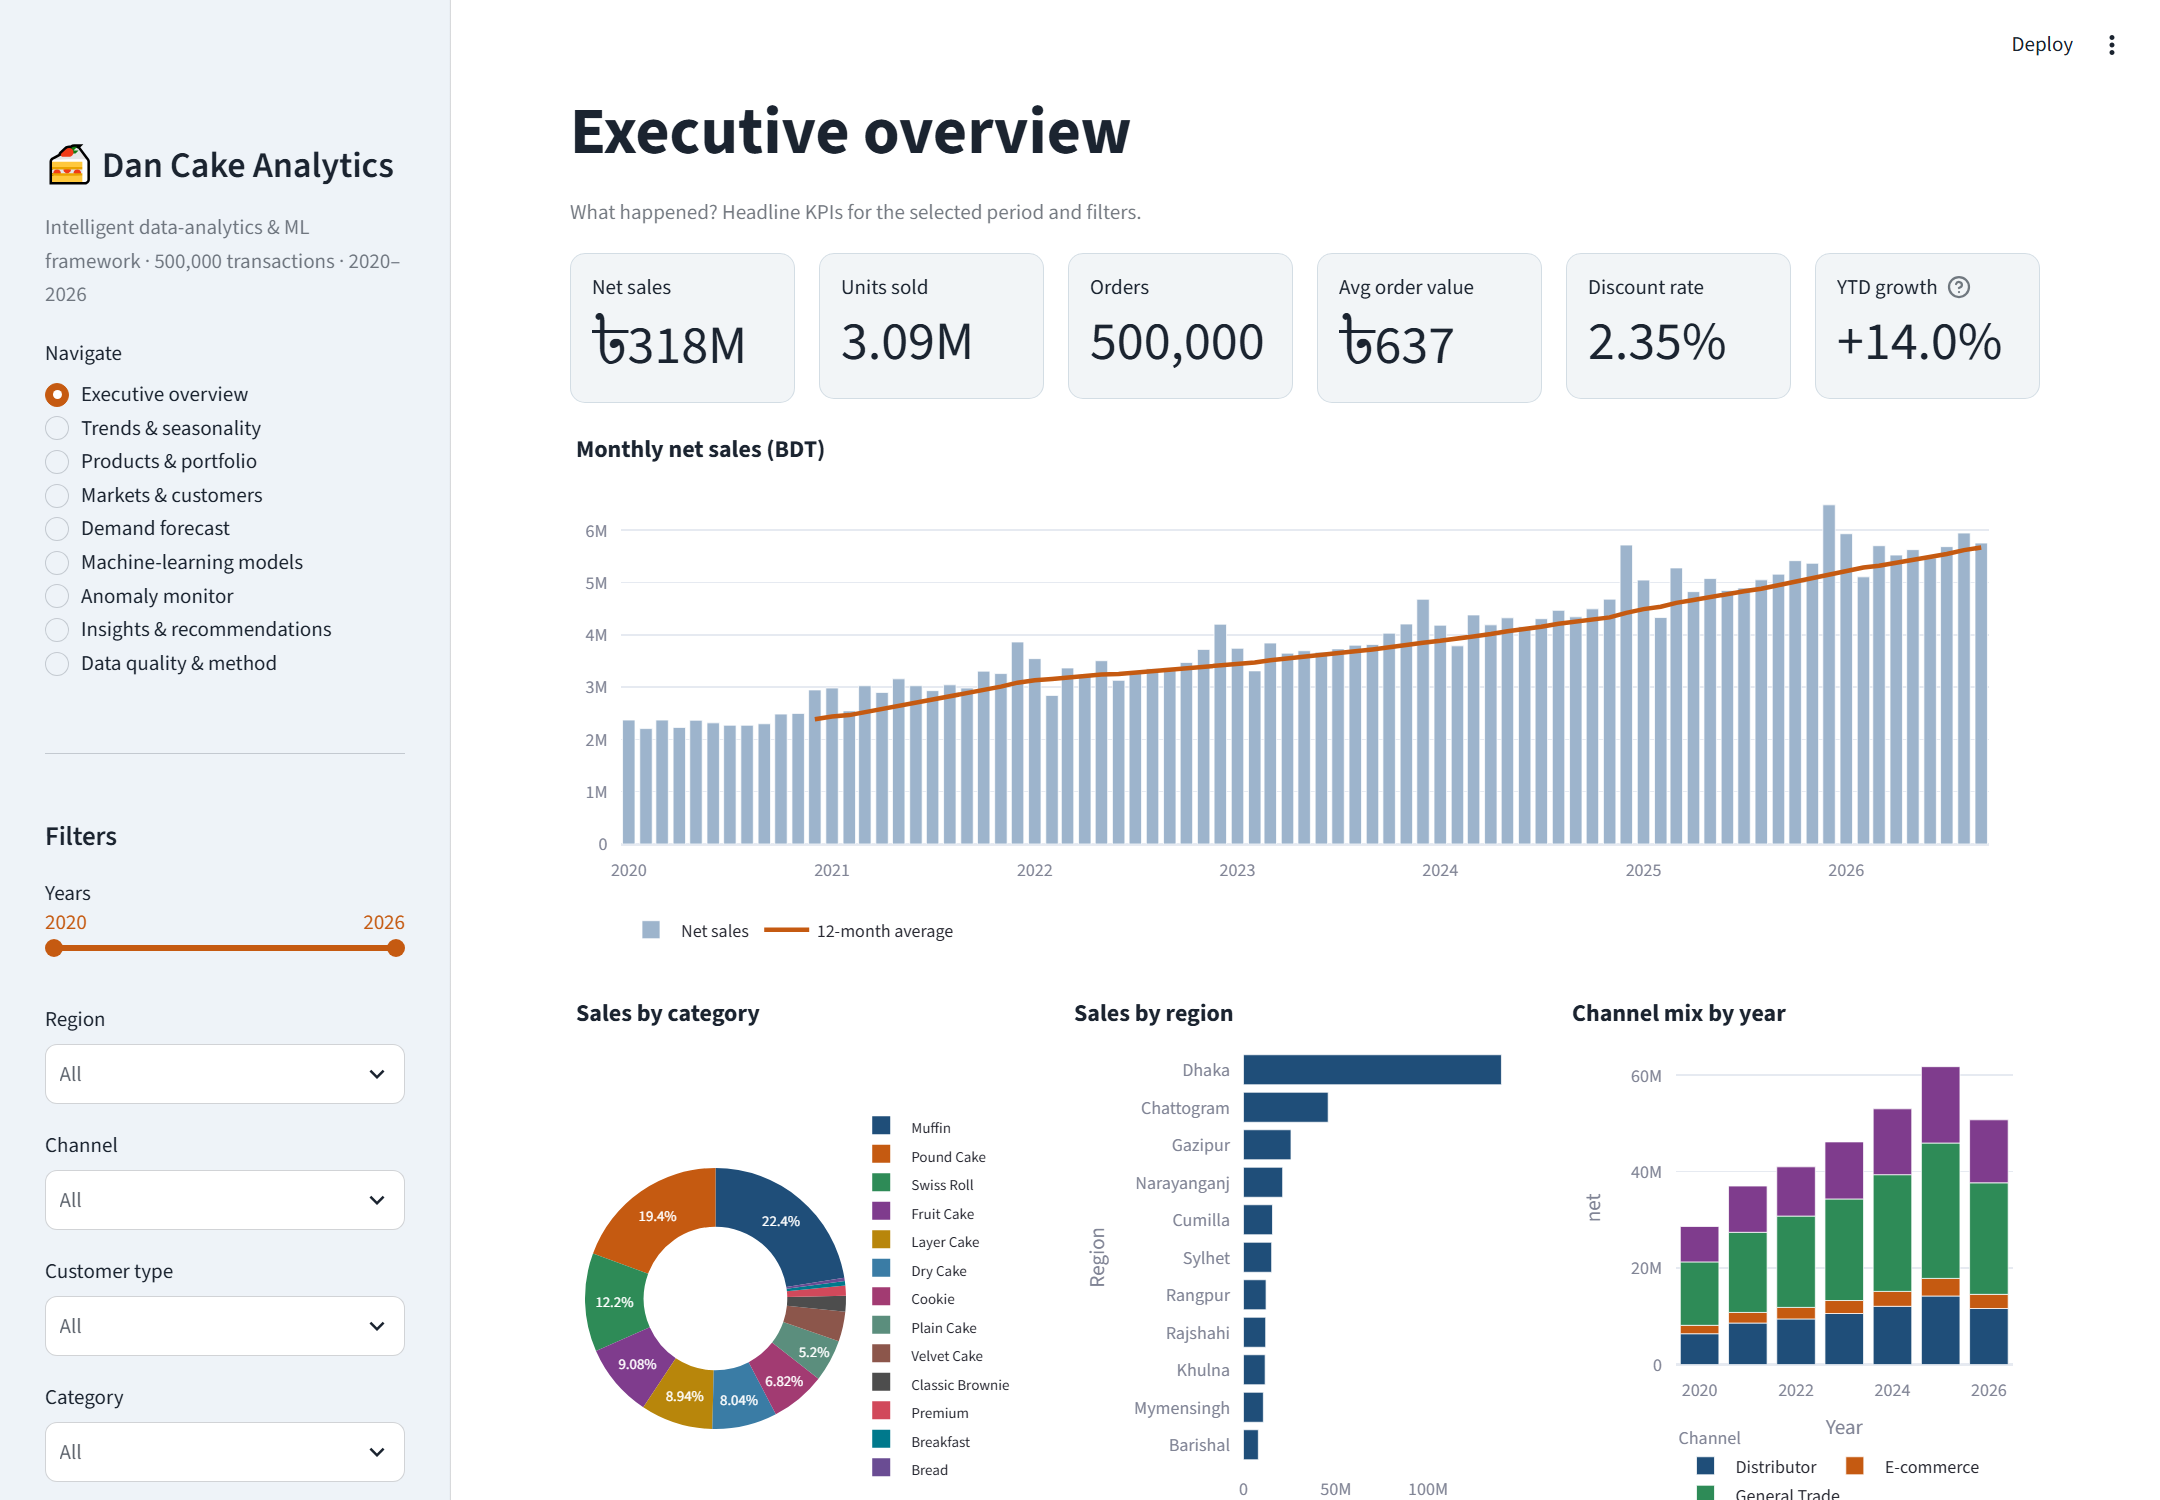
\includegraphics[width=\linewidth]{dash_overview}
\caption{ড্যাশবোর্ডের Executive overview পাতা}\label{fig:dashoverview}
\end{figure}

\begin{figure}[htbp]\centering
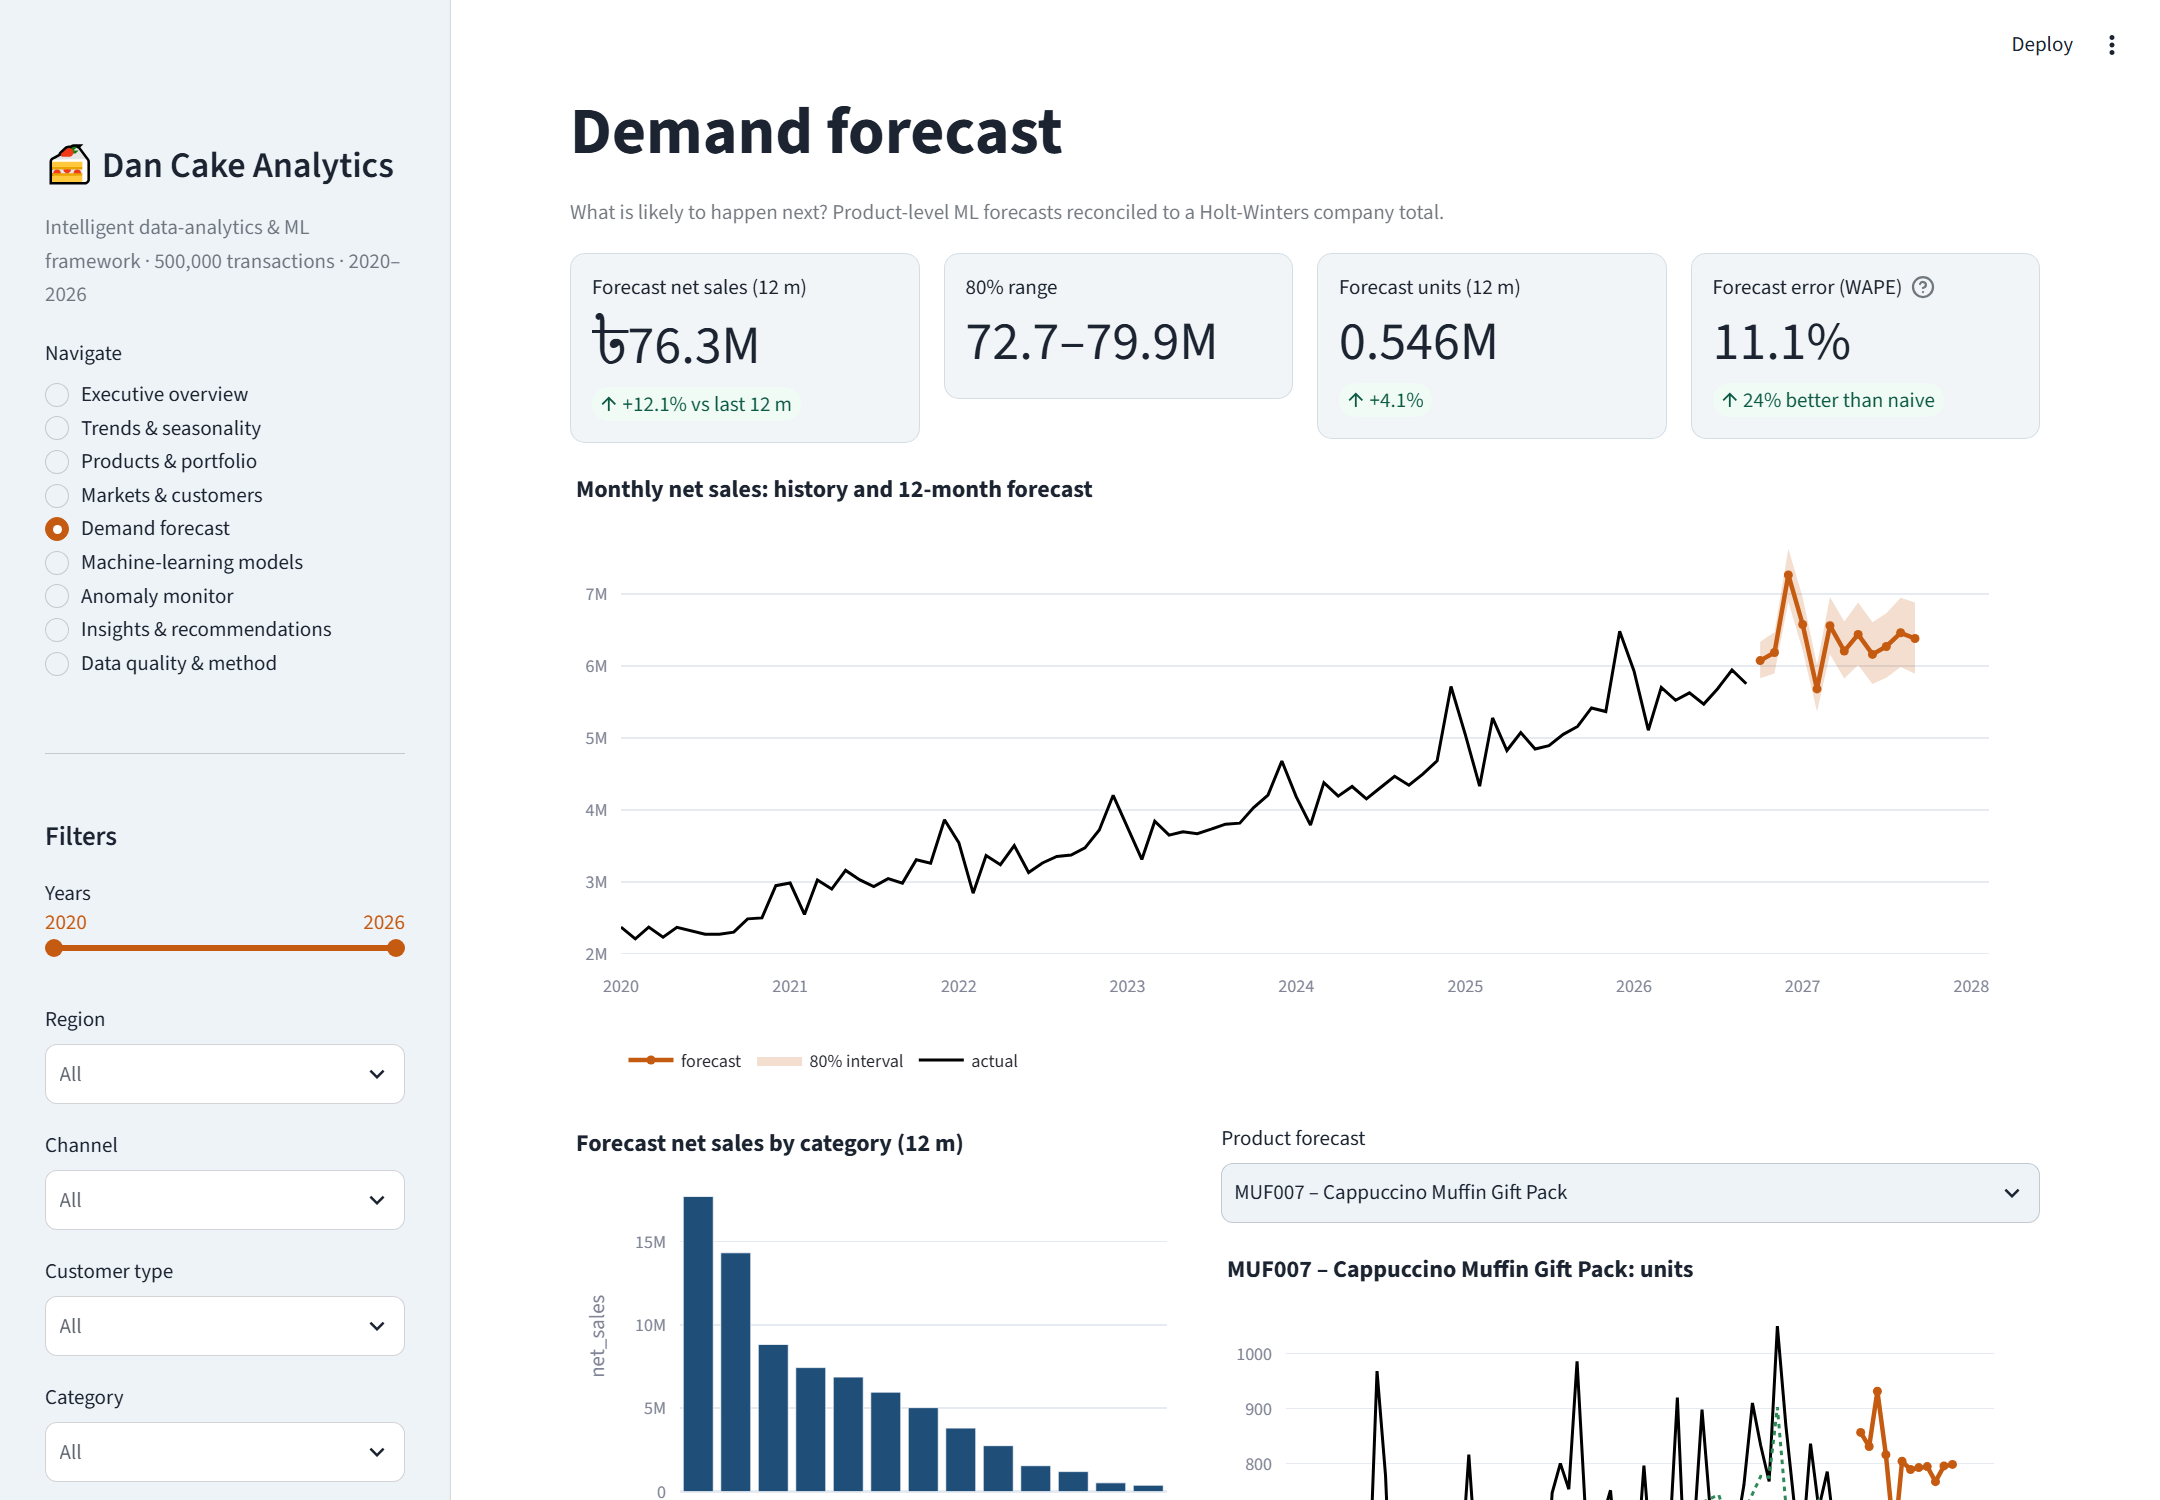
\includegraphics[width=\linewidth]{dash_forecast}
\caption{ড্যাশবোর্ডের চাহিদা-পূর্বাভাস পাতা: 80\% ব্যবধানসহ 12-মাসের দৃষ্টিভঙ্গি}\label{fig:dashforecast}
\end{figure}

\section{প্রকাশ}
দুটি বিনামূল্যের ওয়েব সেবা প্রস্তুত করা হয়েছে:
\begin{itemize}
  \item \textbf{ইন্টারঅ্যাকটিভ ড্যাশবোর্ড}, যা প্রকল্পের GitHub রিপোজিটরি থেকে সরাসরি Streamlit Community Cloud-এ প্রকাশিত
        (ঠিকানার ধরন \dashurl);
  \item একটি \textbf{প্রকল্প ওয়েবসাইট}, \texttt{website.py} দিয়ে তৈরি একটি স্থির পাতা যা GitHub Pages থেকে পরিবেশিত (\siteurl)। এটি
        ইন্টারঅ্যাকটিভ Plotly চার্টসহ প্রকল্পের সারসংক্ষেপ দেয় এবং ড্যাশবোর্ড, সোর্স কোড ও এই প্রতিবেদনের লিংক দেয়।
\end{itemize}
দুটি সেবাই বিনামূল্যে একটি HTTPS সাব-ডোমেইন দেয়। পরে একটি নিজস্ব ডোমেইন কেনা হলে কোড না বদলেই DNS \texttt{CNAME} রেকর্ডের মাধ্যমে তা
GitHub Pages-এ যুক্ত করা যায়। ধাপে ধাপে প্রকাশের পদ্ধতি \cref{app:reproduce}-এ দেওয়া আছে।

\section{সিদ্ধান্ত-সহায়ক স্তর}
শেষ স্তরটি মডেলের ফলাফলকে সুপারিশে রূপান্তর করে। মডিউল \texttt{insights.py} মেট্রিক ফাইলগুলো পড়ে বাক্য-টেমপ্লেটে বর্তমান ফলাফল
বসায়, তাই নতুন ডেটা প্রক্রিয়া হলে প্রতিটি অন্তর্দৃষ্টি হালনাগাদ থাকে এবং কোনোটিই হাতে লেখা হয় না। এই ডেটাসেটের জন্য তৈরি অন্তর্দৃষ্টিগুলো:

\begin{enumerate}[leftmargin=*,itemsep=4pt]
\item \textbf{প্রবৃদ্ধি (কী ঘটেছে)।} 2020 থেকে 2025 পর্যন্ত নিট বিক্রয় বছরে 16.6\% হারে বেড়েছে, কিন্তু ইউনিট বেড়েছে মাত্র 5.0\%; গড়ে বার্ষিক প্রবৃদ্ধির 11.3 শতাংশ-বিন্দু এসেছে মূল্য ও মিশ্রণ থেকে এবং 5.0 পরিমাণ থেকে। \emph{সুপারিশ:} পরিমাণ-প্রবৃদ্ধিকে আলাদা KPI হিসেবে অনুসরণ করুন; মূল্য-নির্ভর প্রবৃদ্ধি অনির্দিষ্টকাল টেকসই নয়।
\item \textbf{মূল্য নির্ধারণ (কেন ঘটেছে)।} পণ্য, বছর ও মৌসুম নিয়ন্ত্রণ করার পর চাহিদার নির্ণীত মূল্য-স্থিতিস্থাপকতা +0.09 (95\% CI -0.28 থেকে +0.46), যা শূন্য থেকে তাৎপর্যপূর্ণভাবে আলাদা নয়। ডিসকাউন্টের সঙ্গে অর্ডারের আকারের কোনো সম্পর্ক নেই (Spearman rho = 0.001)। \emph{সুপারিশ:} ডিসকাউন্ট বাজেট পুনর্বিবেচনা করুন (এই সময়কালে 7.7 মিলিয়ন টাকা): ডিসকাউন্ট বিক্রির পরিমাণ বাড়ায় বলে মনে হয় না।
\item \textbf{মৌসুমিতা (কী ঘটেছে)।} ডিসেম্বর শীর্ষ মাস (সূচক 125, গড় মাস = 100) এবং ফেব্রুয়ারি সবচেয়ে দুর্বল (86)। মৌসুমি প্রভাব পরিসংখ্যানিকভাবে শক্তিশালী (Kruskal-Wallis p < 0.001)। \emph{সুপারিশ:} অক্টোবর থেকে মজুদ ও ডিস্ট্রিবিউটর-সক্ষমতা বাড়ান; ফেব্রুয়ারিতে প্রমোশন ও রক্ষণাবেক্ষণের পরিকল্পনা করুন।
\item \textbf{পোর্টফোলিও (কী ঘটেছে)।} Muffin সবচেয়ে বড় ক্যাটাগরি (বিক্রয়ের 22.4\%); 52টি পণ্যের শীর্ষ 10টি আয়ের 38.5\% দেয় এবং 27টি পণ্য `A' শ্রেণি (বিক্রয়ের 80\%) গঠন করে। \emph{সুপারিশ:} প্রথমে A-শ্রেণির পণ্যের প্রাপ্যতা নিশ্চিত করুন; C-শ্রেণির পণ্য যৌক্তিকীকরণ বা পুনঃস্থাপনের জন্য পর্যালোচনা করুন।
\item \textbf{পোর্টফোলিও (বিভাজন)।} ক্লাস্টারিং 5টি পণ্য-বিভাগ খুঁজে পেয়েছে; `Premium \& gift packs' সবচেয়ে দ্রুত বাড়ছে (বছরে ইউনিট +7.8\%, বিক্রয়ের 33.3\%)। \emph{সুপারিশ:} `Premium \& gift packs'-এর জন্য তাকের জায়গা ও বিপণনে অগ্রাধিকার দিন।
\item \textbf{বাজার (কী ঘটেছে)।} ঢাকা একাই বিক্রয়ের 43.9\% এবং ঢাকা ও চট্টগ্রাম মিলে 58.3\% আনে। General Trade সবচেয়ে বড় চ্যানেল (45.6\%), আর E-commerce 5.9\%। \emph{সুপারিশ:} দ্বিতীয় সারির শহর গড়ে তুলে এবং ছোট ভিত্তি থেকে বাড়তে থাকা E-commerce প্রসারিত করে কেন্দ্রীভবনের ঝুঁকি কমান।
\item \textbf{বাজার (বিভাজন)।} `Emerging high-growth cells' বিভাগটি (19টি অঞ্চল-চ্যানেল-গ্রাহক কোষ, মূলত Cumilla, Khulna, Mymensingh) বছরে +33.2\% হারে বাড়ছে, যা 4টি বাজার-বিভাগের মধ্যে দ্রুততম। \emph{সুপারিশ:} মাঠ-পর্যায়ের বিক্রয় ও ডিজিটাল বিপণনের প্রচেষ্টা এই উদীয়মান কোষগুলোতে বরাদ্দ করুন।
\item \textbf{অর্ডার (পূর্বাভাস)।} একটি অর্ডার বড় হবে কি না ($\geq$ 10 ইউনিট) তা মাঝারি মাত্রায় পূর্বাভাসযোগ্য (সেরা ROC-AUC 0.712, Logistic Regression); চ্যানেলই সবচেয়ে শক্তিশালী চালিকাশক্তি: ডিস্ট্রিবিউটর অর্ডারের 48\% বড়, অথচ অনলাইনে 8\%। \emph{সুপারিশ:} যানবাহন ও মজুদ বণ্টনে বড়-অর্ডার স্কোর ব্যবহার করুন, মূলত চ্যানেল-স্তরে।
\item \textbf{পূর্বাভাস (সামনে কী ঘটবে)।} Support Vector Regression মডেল পরের মাসের পণ্য-চাহিদা 11.1\% weighted ত্রুটিতে পূর্বাভাস করে, যা seasonal-naive নিয়মের চেয়ে 24\% কম RMSE। অক্টোবর 2026 থেকে সেপ্টেম্বর 2027-এর নিট বিক্রয়ের পূর্বাভাস 76.3 মিলিয়ন টাকা (আগের 12 মাসের চেয়ে +12.1\%; 80\% ব্যবধান 72.7 -- 79.9 মিলিয়ন টাকা)। \emph{সুপারিশ:} মাসিক উৎপাদন পরিকল্পনায় পণ্য-স্তরের পূর্বাভাস এবং নিরাপত্তা-মজুদে পূর্বাভাস-ব্যবধান ব্যবহার করুন।
\item \textbf{ঝুঁকি (অস্বাভাবিকতা)।} 2,465টি ব্যবসায়িক দিনের 28টি অস্বাভাবিক হিসেবে চিহ্নিত। একটি নিয়ন্ত্রিত পরীক্ষায় নিয়ম ও Isolation Forest মিলে রোপিত 1,000টি ডেটা-ত্রুটির 91\% ধরেছে। \emph{সুপারিশ:} প্রতিদিন অ্যানোমালি যাচাই চালান এবং মাস-শেষের প্রতিবেদনের আগে চিহ্নিত দিন ও অর্ডার তদন্ত করুন।
\end{enumerate}

প্রতিটি অন্তর্দৃষ্টিকে ক্ষেত্র ও যে ব্যবস্থাপনা প্রশ্নের উত্তর দেয় তা দিয়ে চিহ্নিত করা হয়েছে এবং একটি সুনির্দিষ্ট করণীয়ের সঙ্গে জোড়া দেওয়া হয়েছে।
ফলে ড্যাশবোর্ডটি কেবল প্রতিবেদন-টুল নয়, একটি \emph{সিদ্ধান্ত-সহায়ক ব্যবস্থা}।

\section{সিস্টেম মূল্যায়ন}
প্রস্তাবনায় সিস্টেমটিকে পূর্বাভাস-কর্মদক্ষতা, ব্যবহারযোগ্যতা, বিশ্লেষণী উপযোগিতা, ভিজ্যুয়ালাইজেশনের মান ও প্রক্রিয়াকরণ-দক্ষতায় মূল্যায়ন
করতে বলা হয়েছিল। \Cref{tab:syseval} প্রমাণগুলোর সারসংক্ষেপ দেয়।

\begin{table}[htbp]\centering\small
\caption{প্রস্তাবনার মানদণ্ডে কাঠামোর মূল্যায়ন}\label{tab:syseval}
\begin{tabularx}{\linewidth}{@{}lX@{}}
\toprule
\textbf{মানদণ্ড} & \textbf{প্রমাণ} \\ \midrule
পূর্বাভাস-কর্মদক্ষতা & সব ML পূর্বাভাসক naive বেঞ্চমার্ককে হারিয়েছে; সেরা WAPE \BestRegWAPE\%; কোম্পানি-পর্যায়ে MAPE \HWMAPE\%;
ক্লাসিফিকেশনে ROC-AUC \ClsAUC (\cref{ch:models}) \\
বিশ্লেষণী উপযোগিতা & প্রবৃদ্ধির মান, ডিসকাউন্টের অকার্যকারিতা, মৌসুমিতা, কেন্দ্রীভবনের ঝুঁকি, বিভাগ ও অস্বাভাবিকতা বিষয়ে অন্তর্দৃষ্টি, প্রতিটির সঙ্গে
করণীয় \\
ব্যবহারযোগ্যতা & এক সেট সর্বজনীন ফিল্টার; কাজভিত্তিক নয়টি পাতা; সহজ ভাষার ক্যাপশন; ডাউনলোডযোগ্য পূর্বাভাস; ইনস্টলেশন ছাড়াই যেকোনো
ব্রাউজারে চলে \\
ভিজ্যুয়ালাইজেশনের মান & Few-এর নীতি: KPI কার্ড, সাজানো বার, heat map, পূর্বাভাসে ব্যবধান, কোনো 3-D বা সাজসজ্জামূলক চার্ট নয়, সামঞ্জস্যপূর্ণ
রং \\
প্রক্রিয়াকরণ-দক্ষতা & \NRows সারির যাচাই ও পরিষ্কারকরণ 20 সেকেন্ডের কম সময়ে; ওয়্যারহাউস লোড \WarehouseSeconds সেকেন্ডে; মডেল টিউনিংসহ
পুরো পাইপলাইন একটি সাধারণ ল্যাপটপে প্রায় 20 মিনিটে; ড্যাশবোর্ড-ডেটা প্রায় 2 MB \\
পুনরুৎপাদনযোগ্যতা & একটি কমান্ডে সব ডেটা, মডেল, চিত্র, সারণি ও সংখ্যা পুনরায় তৈরি; নির্দিষ্ট random seed; স্বয়ংক্রিয় টেস্ট \\ \bottomrule
\end{tabularx}
\end{table}

ব্যবস্থাপকদের নিয়ে একটি আনুষ্ঠানিক ব্যবহারযোগ্যতা-গবেষণা হাতে থাকা সময়ের মধ্যে সম্ভব হয়নি। এটি ভবিষ্যৎ কাজ হিসেবে সুপারিশ করা হচ্ছে:
System Usability Scale প্রশ্নমালাসহ একটি সংক্ষিপ্ত কাজভিত্তিক পরীক্ষা মূল্যায়ন সম্পূর্ণ করবে।

\chapter{আলোচনা}\label{ch:discussion}

\section{গবেষণা প্রশ্নের উত্তর}

\paragraph{RQ1: ডেটা অ্যানালিটিক্স কীভাবে ব্যবসায়িক সিদ্ধান্ত গ্রহণ উন্নত করতে পারে?}
কাঠামোটি অ্যানালিটিক্সের তিনটি স্তরেই উন্নতি দেখায়। \emph{বর্ণনামূলক} স্তরে এটি হাতে-করা স্প্রেডশিট একত্রীকরণের বদলে যাচাইকৃত ও
মিলানো KPI দেয়, যা একটি কমান্ডে হালনাগাদ হয়। \emph{রোগনির্ণয়মূলক} স্তরে এটি এমন সম্পর্ক উন্মোচন করে যা সাধারণ প্রতিবেদনে চোখ
এড়িয়ে যেত: প্রবৃদ্ধি মূলত মূল্য ও মিশ্রণ-চালিত; ডিসকাউন্ট বড় অর্ডারের সঙ্গে যুক্ত নয়; অর্ডারের আকার গ্রাহকের ধরন নয়, চ্যানেলের উপর নির্ভর
করে। \emph{পূর্বাভাসমূলক} স্তরে এটি পরিমাপিত অনিশ্চয়তাসহ পণ্য-স্তরের পূর্বাভাস দেয়। এর প্রতিটি একটি সুনির্দিষ্ট সিদ্ধান্ত বদলায়: ডিসকাউন্ট
বাজেট, বিক্রয়-বাহিনী বণ্টন, উৎপাদন পরিকল্পনা ও লজিস্টিক সক্ষমতা।

\paragraph{RQ2: কোন প্রিপ্রসেসিং কৌশল সবচেয়ে কার্যকর?}
তিনটি কৌশল সবচেয়ে মূল্যবান প্রমাণিত হয়েছে। প্রথমত, হিসাবগত অভেদ থেকে অনুপস্থিত মান \emph{নির্ণয়}, যা হুবহু পুনরুদ্ধার দেয় এবং
পরিসংখ্যানিক imputation-এর আগে সবসময় চেষ্টা করা উচিত। দ্বিতীয়ত, \emph{robust, দলভিত্তিক outlier শনাক্তকরণ} (log স্কেলে প্রতি-পণ্য
IQR), যা বিষম বণ্টন ও ভিন্ন পণ্য-স্কেলকে সম্মান করে; অস্বাভাবিক মান মুছে না ফেলে চিহ্নিত করার নীতির সঙ্গে মিলে এটি প্রকৃত বাল্ক অর্ডারগুলো
রক্ষা করে। তৃতীয়ত, \emph{leakage-মুক্ত ফিচার ইঞ্জিনিয়ারিং}, যেখানে rolling-এর আগে ইতিহাস-ফিচার shift করা হয় এবং প্রতিটি শেখা প্যারামিটার
কেবল প্রশিক্ষণ ডেটায় fit করা হয়। ব্যবসায়িক চলকগুলো অত্যন্ত বিষম হওয়ায় সর্বত্র normal-তত্ত্বের পদ্ধতির চেয়ে robust পদ্ধতি শ্রেয় ছিল।

\paragraph{RQ3: কোন অ্যালগরিদম সবচেয়ে ভালো?}
সব সমস্যায় একটি অ্যালগরিদম সেরা নয়, এবং ভালো মডেলগুলোর ব্যবধান সামান্য। এক মাস অগ্রিম পণ্য-চাহিদায় \BestReg সবচেয়ে নির্ভুল ছিল;
বহু-ধাপ পরিস্থিতিতে \BestRec সবচেয়ে দৃঢ়; কোম্পানি-পর্যায়ে ধ্রুপদী Holt--Winters মডেল সব মেশিন লার্নিং বিকল্পকে হারিয়েছে; আর
ক্লাসিফিকেশনে logistic regression tree ensemble-এর সমান। এই ধারা \citet{makridakis2018}-এর সঙ্গে মেলে: অ্যালগরিদম বাছাইয়ের চেয়ে
ভালো ফিচার, সঠিক যাচাই-নকশা ও বেঞ্চমার্ক বেশি গুরুত্বপূর্ণ। ব্যবহারিকভাবে সবচেয়ে উপযোগী একটি সমন্বিত পদ্ধতি: পরিসংখ্যানিক মোট, মেশিন
লার্নিং দিয়ে শেখা পণ্য-মিশ্রণে মিলানো।

\paragraph{RQ4: ঐতিহাসিক ডেটায় কী প্যাটার্ন আছে?}
ডিসেম্বরে শীর্ষে পৌঁছানো শক্তিশালী বছর-শেষের মৌসুমিতা; স্থির কিন্তু মূল্য-চালিত প্রবৃদ্ধি ও মূল্য-অস্থিতিস্থাপক চাহিদা; ঢাকা ও চট্টগ্রামে
ভৌগোলিকভাবে এবং প্রায় দশটি পণ্যে পোর্টফোলিও-গতভাবে কেন্দ্রীভূত আয়; চ্যানেলভেদে অর্ডারের আকারে বড় পার্থক্য; ডিসকাউন্টের কোনো শনাক্তযোগ্য
পরিমাণ-প্রভাব নেই; এবং সপ্তাহের দিনের প্রভাব নেই। বিভাজন যোগ করে একটি পোর্টফোলিও-দৃষ্টিভঙ্গি (প্রিমিয়াম ও গিফট প্যাক, কোর ফ্যামিলি
প্যাক, ভ্যালু সিঙ্গেল-সার্ভ ও নিশ লাইন) এবং একটি বাজার-দৃষ্টিভঙ্গি (core retail, bulk distribution, online ও আঞ্চলিক, উদীয়মান
উচ্চ-প্রবৃদ্ধি)।

\paragraph{RQ5: ভবিষ্যৎ কতটা নির্ভুলভাবে পূর্বাভাস করা যায়?}
প্রতিটি পণ্যের মাসিক চাহিদা এক মাস অগ্রিম প্রায় \BestRegWAPE\% এবং 21 মাস পর্যন্ত প্রায় \BestRecWAPE\% weighted ত্রুটিতে পূর্বাভাস করা
যায়; কোম্পানি-স্তরের মাসিক ইউনিট প্রায় \HWMAPE\% ত্রুটিতে। একটি নির্দিষ্ট অর্ডার বড় হবে কি না তা কেবল মাঝারি মাত্রায় পূর্বাভাসযোগ্য
(ROC-AUC \ClsAUC); সীমাবদ্ধতা মডেলে নয়, প্রাপ্ত তথ্যে।

\paragraph{RQ6: ব্যবস্থাপকদের কাছে ফলাফল কীভাবে উপস্থাপন করা উচিত?}
ব্যবস্থাপনা প্রশ্নগুলোকে ঘিরে সাজানো একটি ইন্টারঅ্যাকটিভ ড্যাশবোর্ডের মাধ্যমে, যেখানে সর্বজনীন ফিল্টার, KPI কার্ড ও সরল সাজানো চার্ট থাকবে,
পূর্বাভাসে সবসময় অনিশ্চয়তা দেখানো হবে, এবং প্রতিটি অন্তর্দৃষ্টি একটি করণীয়সহ সহজ ভাষায় বলা হবে। বিনামূল্যের প্ল্যাটফর্মে ড্যাশবোর্ড ও
সারসংক্ষেপ ওয়েবসাইট প্রকাশ করলে খরচ ও ইনস্টলেশনের বাধা দূর হয়।

\paragraph{RQ7: ঐতিহাসিক প্রতিবেদনের তুলনায় পূর্বাভাসমূলক অ্যানালিটিক্স কতটা যোগ করে?}
একটি ঐতিহাসিক প্রতিবেদন বড়জোর গত বছরের প্যাটার্ন পুনরাবৃত্তি করতে পারে, যা seasonal-naive নিয়ম। মেশিন লার্নিং পূর্বাভাস এর ত্রুটি
\GainVsSNaive\% কমায়। অন্যভাবে বললে, গত বছরের হিসাব দিয়ে পরিকল্পনাকারী প্রতি পণ্য-মাসে পরিমাণের প্রায় \SNaiveWAPE\% ভুল করতেন, যেখানে
এই কাঠামোয় তা \BestRegWAPE\%। এর উপর, পূর্বাভাস-ব্যবধান এমন তথ্য যোগ করে যা ঐতিহাসিক প্রতিবেদন একেবারেই দিতে পারে না: কতটা
নিরাপত্তা-মজুদ রাখতে হবে।

\section{ব্যবস্থাপনাগত তাৎপর্য}
\begin{itemize}
  \item \textbf{মূল্য ও প্রমোশন।} চাহিদা অস্থিতিস্থাপক এবং ডিসকাউন্ট অর্ডারের আকার বাড়ায় না। এই সময়কালে প্রায় \DiscountCost মিলিয়ন টাকার
        ডিসকাউন্ট বাজেট পুনর্বিবেচনা করা উচিত, এবং নিয়ন্ত্রিত পরীক্ষার (A/B প্রমোশন) মাধ্যমে যাচাই করা উচিত লক্ষ্যভিত্তিক প্রমোশন লাভজনক কি না।
  \item \textbf{পরিমাণ-প্রবৃদ্ধি।} প্রবৃদ্ধি মূল্য-নির্ভর হওয়ায় পরিমাণকে আলাদা KPI হিসেবে অনুসরণ করা উচিত, এবং কম-প্রবেশিত অঞ্চল ও
        E-commerce-এ প্রবৃদ্ধির উদ্যোগ নেওয়া উচিত।
  \item \textbf{মৌসুমি পরিকল্পনা।} ডিসেম্বরের শীর্ষের জন্য অক্টোবর থেকে উৎপাদন ও ডিস্ট্রিবিউটর-মজুদ বাড়াতে হবে; ফেব্রুয়ারি রক্ষণাবেক্ষণ ও
        প্রমোশনের স্বাভাবিক সময়।
  \item \textbf{পোর্টফোলিও।} A-শ্রেণির পণ্যগুলো সর্বোচ্চ সেবা-স্তরের যোগ্য; C-শ্রেণির পণ্যগুলো পর্যালোচনার প্রার্থী।
  \item \textbf{লজিস্টিকস।} বড় অর্ডার ডিস্ট্রিবিউটর চ্যানেল ও নির্দিষ্ট অঞ্চলে কেন্দ্রীভূত, তাই যানবাহন ও মজুদ বণ্টন সেই স্তরে পরিকল্পনা করা যায়।
  \item \textbf{নিয়ন্ত্রণ।} দৈনিক অ্যানোমালি যাচাই ডেটার মান উন্নত করে এবং পরিচালনাগত সমস্যা আগেভাগে ধরে।
\end{itemize}

\section{সীমাবদ্ধতা}\label{sec:limitations}
\begin{itemize}
  \item \textbf{ডেটার উৎস ও বাস্তবতা।} ডেটাসেটটি অত্যন্ত পরিষ্কার: কোনো অনুপস্থিত মান নেই, হিসাবগত অভেদ হুবহু মেলে, এবং অর্ডারের আকার
        গ্রাহকের ধরন, ডিসকাউন্ট ও পণ্য থেকে প্রায় স্বাধীন। বাস্তব পরিচালনাগত ডেটা সাধারণত এর চেয়ে অগোছালো। তাই পাইপলাইনটি ইচ্ছাকৃতভাবে
        নষ্ট করা অনুলিপিতে পরীক্ষা করা হয়েছে, তবে গ্রাহক-আচরণ সম্পর্কিত সিদ্ধান্তে পদক্ষেপ নেওয়ার আগে কোম্পানির আরও ডেটায় যাচাই করা উচিত।
        ডেটাসেটের সঠিক উৎস ও সংগ্রহ-প্রক্রিয়া এই প্রতিবেদনের সঙ্গে নথিভুক্ত করা উচিত।
  \item \textbf{অনুপস্থিত চালিকাশক্তি।} বিপণন-ব্যয়, প্রতিযোগীর মূল্য, মজুদ-ঘাটতি, আবহাওয়া বা ছুটির কোনো ডেটা পাওয়া যায়নি; এগুলো যুক্ত হলে
        পূর্বাভাস ও ক্লাসিফিকেশন উভয়ই সম্ভবত উন্নত হবে।
  \item \textbf{পর্যবেক্ষণভিত্তিক স্থিতিস্থাপকতা।} স্থিতিস্থাপকতার অনুমান সময়ের সঙ্গে তালিকা-মূল্যের পরিবর্তনের উপর নির্ভরশীল, এলোমেলো পরীক্ষার
        উপর নয়; মূল্য সামান্য পরিমাণে বদলেছে, তাই পর্যবেক্ষিত সীমার বাইরে স্থিতিস্থাপকতা অজানা।
  \item \textbf{ভবিষ্যৎ পরিস্থিতি।} সব পূর্বাভাস ধরে নেয় অতীতের প্যাটার্ন চলবে; কাঠামোগত পরিবর্তন (যেমন নতুন প্রতিযোগী বা অর্থনৈতিক ধাক্কা)
        নির্ভুলতা কমাবে।
  \item \textbf{মূল্যায়নের পরিধি।} ড্যাশবোর্ডটি এখনো প্রকৃত ব্যবস্থাপকদের দিয়ে মূল্যায়িত হয়নি; আর প্যানেলটি (52টি সিরিজ, 81 মাস) এত ছোট যে
        deep-learning মডেল ব্যবহারের যৌক্তিকতা নেই, তাই সেগুলো পরীক্ষা করা হয়নি।
\end{itemize}

\section{পদ্ধতি নিয়ে প্রতিফলন}
সবচেয়ে গুরুত্বপূর্ণ পদ্ধতিগত সিদ্ধান্ত ছিল বেঞ্চমার্কসহ কঠোর সময়-ক্রমিক মূল্যায়ন; এলোমেলো cross-validation চমৎকার কিন্তু বিভ্রান্তিকর
নির্ভুলতার সংখ্যা দিত। কোড থেকে প্রতিটি উল্লিখিত সংখ্যা তৈরি করাও মূল্যবান প্রমাণিত হয়েছে: কাজ এগোনোর সঙ্গে বিশ্লেষণ বহুবার পুনরায় চালানো
হয়েছে, এবং প্রতিবেদন সবসময় সামঞ্জস্যপূর্ণ থেকেছে। এ ধরনের ভবিষ্যৎ প্রকল্পে দুটি চর্চাই সুপারিশযোগ্য।

\chapter{উপসংহার ও ভবিষ্যৎ কাজ}\label{ch:conclusion}

\section{উপসংহার}
এই প্রকল্পের লক্ষ্য ছিল এমন একটি বুদ্ধিমান ডেটা অ্যানালিটিক্স ও মেশিন লার্নিং কাঠামো নকশা ও উন্নয়ন করা, যা কাঁচা ব্যবসায়িক ডেটাকে কার্যকর
অন্তর্দৃষ্টি ও পূর্বাভাসমূলক তথ্যে রূপান্তর করে। সাতটি উদ্দেশ্যই পূরণ হয়েছে। \NRows লেনদেনের একটি ডেটাসেট যাচাই, পরিষ্কার ও একটি
ডাইমেনশনাল ডেটাবেসে সংরক্ষণ করা হয়েছে (O1, O2)। অনুসন্ধানমূলক ও অনুমানমূলক বিশ্লেষণে উন্মোচিত হয়েছে মূল্য-চালিত প্রবৃদ্ধি,
অস্থিতিস্থাপক চাহিদা, অকার্যকর ডিসকাউন্ট, শক্তিশালী বছর-শেষের মৌসুমিতা এবং উচ্চ ভৌগোলিক ও পোর্টফোলিও কেন্দ্রীভবন (O3)। সাতটি রিগ্রেশন
ও সাতটি ক্লাসিফিকেশন অ্যালগরিদম, তিনটি ক্লাস্টারিং পদ্ধতি, পরিসংখ্যানিক পূর্বাভাস মডেল এবং দুটি অ্যানোমালি ডিটেক্টর একটি কঠোর
সময়-ক্রমিক পদ্ধতিতে তৈরি ও তুলনা করা হয়েছে (O4)। ফলাফল একটি বিনামূল্যে, প্রকাশ্যে হোস্ট করা ইন্টারঅ্যাকটিভ ড্যাশবোর্ড ও প্রকল্প
ওয়েবসাইটে উপস্থাপিত (O5), স্বয়ংক্রিয়ভাবে তৈরি অন্তর্দৃষ্টি ও সুপারিশসহ (O6)। কাঠামোর পূর্বাভাস-কর্মদক্ষতা, উপযোগিতা, দক্ষতা ও
পুনরুৎপাদনযোগ্যতা মূল্যায়ন করা হয়েছে (O7)।

কেন্দ্রীয় উপসংহার হলো, সবচেয়ে বড় মূল্য আসে সবচেয়ে জটিল অ্যালগরিদম থেকে নয়, বরং \emph{একীকরণ} ও \emph{শৃঙ্খলা} থেকে। পরিষ্কার ও যাচাইকৃত
ডেটা, leakage-মুক্ত ফিচার, সৎ বেঞ্চমার্ক এবং স্পষ্ট যোগাযোগ সরল ও সুপরিচিত মডেলগুলোকে নির্ভরযোগ্য সিদ্ধান্ত-সহায়তায় পরিণত করেছে। সেরা
পণ্য-স্তরের পূর্বাভাস ``গত বছরের মতো'' পরিকল্পনার ত্রুটি \GainVsSNaive\% কমিয়েছে, এবং ধ্রুপদী ও মেশিন লার্নিং পদ্ধতি একসঙ্গে সবচেয়ে
ভালো কাজ করেছে। এভাবে প্রতিষ্ঠানটি অতীত বর্ণনা থেকে ভবিষ্যৎ অনুমানের দিকে এগোতে পারে, একটি ব্যবস্থার ভেতরেই \emph{কী ঘটেছে},
\emph{কেন} এবং \emph{সামনে কী} প্রশ্নের উত্তর দিয়ে।

\section{ভবিষ্যৎ কাজ}
\begin{itemize}
  \item \textbf{সমৃদ্ধ ডেটা:} প্রমোশন, বিপণন-ব্যয়, প্রতিযোগীর মূল্য, মজুদ ও মজুদ-ঘাটতি, সরকারি ছুটি (ঈদ, পহেলা বৈশাখ) ও আবহাওয়ার ডেটা
        API-এর মাধ্যমে যুক্ত করা।
  \item \textbf{রিয়েল-টাইম অ্যানালিটিক্স ও সতর্কবার্তা:} ক্লাউডে প্রতিদিন পাইপলাইন চালানো এবং অস্বাভাবিকতা ও পূর্বাভাস-বিচ্যুতির সতর্কবার্তা ই-মেইল
        বা মেসেজে পাঠানো।
  \item \textbf{MLOps:} ডেটা ও মডেলের সংস্করণ রাখা, সময়ের সঙ্গে পূর্বাভাসের নির্ভুলতা পর্যবেক্ষণ করা এবং কর্মদক্ষতা কমলে স্বয়ংক্রিয়ভাবে
        পুনঃপ্রশিক্ষণ।
  \item \textbf{নির্দেশমূলক অ্যানালিটিক্স:} পূর্বাভাস-ব্যবধান ব্যবহার করে সক্ষমতার সীমার মধ্যে উৎপাদনের পরিমাণ ও ডিস্ট্রিবিউটর-বণ্টন অপ্টিমাইজ করা।
  \item \textbf{প্রমোশনের কার্যকারণ মূল্যায়ন:} ডিসকাউন্টের প্রকৃত প্রভাব মাপতে নিয়ন্ত্রিত প্রমোশন-পরীক্ষা চালানো।
  \item \textbf{উন্নত মডেল:} পণ্য, অঞ্চল ও চ্যানেল জুড়ে hierarchical reconciliation, এবং দীর্ঘতর ও বিস্তারিত ইতিহাস পাওয়া গেলে global
        deep-learning পূর্বাভাসক।
  \item \textbf{জেনারেটিভ-AI সহকারী:} ব্যবস্থাপকরা সাধারণ ভাষায় প্রশ্ন করবেন (যেমন ``মার্চে রংপুরে বিক্রয় কমল কেন?'') এবং কাঠামোর ডেটা
        ও মেট্রিক-ভিত্তিক উত্তর পাবেন।
  \item \textbf{ব্যবহারযোগ্যতা-গবেষণা:} কাজভিত্তিক পরীক্ষা ও System Usability Scale দিয়ে ব্যবস্থাপকদের সঙ্গে ড্যাশবোর্ড মূল্যায়ন।
\end{itemize}


\bibliographystyle{plainnat}
\bibliography{references}

\appendix
\chapter{ডেটা অভিধান}\label{app:dictionary}
\begin{table}[htbp]\centering\footnotesize
\caption{লেনদেন ডেটাসেটের ডেটা অভিধান}\label{tab:dictionary}
\begin{tabularx}{\linewidth}{@{}llX@{}}
\toprule
\textbf{কলাম} & \textbf{ধরন} & \textbf{বিবরণ} \\ \midrule
Transaction\_ID & টেক্সট & অনন্য লেনদেন শনাক্তকারী (যেমন DC2020000000) \\
Date & তারিখ & লেনদেনের তারিখ (dd-mm-yy) \\
Year, Month, Month\_Name, Quarter & পূর্ণসংখ্যা/টেক্সট & তারিখ থেকে নির্ণীত ক্যালেন্ডার-বৈশিষ্ট্য \\
Product\_ID, Product\_Name & টেক্সট & পণ্যের কোড ও নাম (\NProducts টি পণ্য) \\
Category & টেক্সট & পণ্যের ক্যাটাগরি (13টি) \\
Pack\_Size & টেক্সট & প্যাক সাইজ, যেমন 30g, 27--30g, 30g x 12, 5 pcs \\
Product\_Launch\_Year & পূর্ণসংখ্যা & পণ্য চালুর বছর \\
Observed\_Price\_BDT & পূর্ণসংখ্যা & মুদ্রিত সর্বোচ্চ খুচরা মূল্য \\
List\_Price\_BDT & পূর্ণসংখ্যা & বছরের কোম্পানি-নির্ধারিত তালিকা মূল্য \\
Market\_Price\_BDT & দশমিক & ডিসকাউন্টের আগে লেনদেন-মূল্য \\
Discount\_\% & দশমিক & ডিসকাউন্টের শতাংশ \\
Unit\_Selling\_Price\_BDT & দশমিক & ডিসকাউন্টের পরে একক মূল্য \\
Quantity & পূর্ণসংখ্যা & বিক্রীত ইউনিট \\
Gross\_Sales\_BDT & দশমিক & পরিমাণ $\times$ বাজার মূল্য \\
Discount\_BDT & দশমিক & ডিসকাউন্টের পরিমাণ \\
Net\_Sales\_BDT & দশমিক & মোট বিক্রয় $-$ ডিসকাউন্ট \\
Region & টেক্সট & বাংলাদেশের 11টি অঞ্চলের একটি \\
Channel & টেক্সট & General Trade, Modern Trade, Distributor, E-commerce \\
Customer\_Type & টেক্সট & Retailer, Super Shop, Distributor, Corporate, Online Customer \\ \bottomrule
\end{tabularx}
\end{table}

\chapter{টিউন করা Hyper-parameter}\label{app:hyper}
\begin{table}[htbp]
\centering
\footnotesize
\caption{Expanding-window যাচাইসহ randomised search-এ নির্বাচিত hyper-parameter (চাহিদা পূর্বাভাস)}
\label{tab:hyper}
\begin{adjustbox}{max width=\linewidth}
\begin{tabular}{l>{\raggedright\arraybackslash}p{10cm}}
\toprule
\textbf{Model} & \textbf{Selected hyper-parameters} \\
\midrule
Linear Regression & none (closed form) \\
Decision Tree & max\_depth=10, min\_samples\_leaf=40 \\
Random Forest & max\_depth=None, max\_features=0.33, min\_samples\_leaf=2, n\_estimators=500 \\
Gradient Boosting & learning\_rate=0.05, max\_depth=2, n\_estimators=200, subsample=1.0 \\
XGBoost & colsample\_bytree=0.6, learning\_rate=0.02, max\_depth=3, min\_child\_weight=10, n\_estimators=600, reg\_lambda=1, subsample=0.9 \\
K-Nearest Neighbors & n\_neighbors=20, weights=distance \\
Support Vector Regression & C=0.3, epsilon=0.05, gamma=0.01 \\
\bottomrule
\end{tabular}
\end{adjustbox}
\end{table}

\chapter{উদাহরণ SQL কোয়েরি}\label{app:sql}
নিচের কোয়েরিগুলো স্টার স্কিমায় (\cref{fig:star}) চলে এবং \cref{ch:eda}-এর প্রধান সংখ্যাগুলো সরাসরি SQL-এ পুনরুৎপাদন করে। এগুলো একটি
Power BI প্রতিবেদনের ডেটা-উৎস হিসেবেও ব্যবহার করা যায়।
\lstinputlisting[language=SQL]{sql/kpi_queries.sql}

\chapter{প্রকল্পটি পুনরুৎপাদন ও প্রকাশ}\label{app:reproduce}
\section{প্রকল্পের কাঠামো}
\begin{lstlisting}
dan_cake_project/
  run_pipeline.py          one command for the whole framework
  src/dancake/             config, data, eda, features, forecasting, classification,
                           clustering, anomaly, insights, export, website
  dashboard/app.py         Streamlit dashboard
  data/  processed/ warehouse/ dashboard/   generated data
  outputs/ metrics/ tables/ models/          generated results
  report/  main.tex, main_bn.tex, chapters/, chapters_bn/, figures/, tables/, tables_bn/
  docs/                    project website (GitHub Pages)
  sql/  tests/  guides/
\end{lstlisting}

\section{নিজের কম্পিউটারে চালানো}
\begin{lstlisting}[language=bash]
python -m venv .venv
.venv\Scripts\activate            # Windows  (source .venv/bin/activate on macOS/Linux)
pip install -r requirements.txt
python run_pipeline.py            # about 20 minutes
python -m pytest tests            # automated tests
streamlit run dashboard/app.py    # open http://localhost:8501
\end{lstlisting}
বাংলা প্রতিবেদন XeLaTeX দিয়ে কম্পাইল করতে হয়: \texttt{tectonic -X compile main\_bn.tex}, অথবা Overleaf-এ Compiler = XeLaTeX।

\section{বিনামূল্যে প্রকাশ}
\begin{enumerate}
  \item একটি বিনামূল্যের GitHub অ্যাকাউন্ট ও একটি পাবলিক রিপোজিটরি তৈরি করে প্রকল্পটি push করুন (\texttt{.gitignore} কাঁচা CSV বাদ দেয়;
        ছোট ড্যাশবোর্ড-ডেটা অন্তর্ভুক্ত থাকে)।
  \item \textbf{ড্যাশবোর্ড:} GitHub দিয়ে Streamlit Community Cloud-এ সাইন ইন করে \emph{New app} বেছে নিন, রিপোজিটরি, branch
        \texttt{main} ও ফাইল \texttt{dashboard/app.py} নির্বাচন করে deploy করুন। অ্যাপটি \texttt{.streamlit.app}-এ শেষ হওয়া একটি ঠিকানা পাবে।
  \item \textbf{ওয়েবসাইট:} রিপোজিটরির settings-এ \emph{Pages} খুলে \emph{Deploy from a branch}, branch \texttt{main}, folder
        \texttt{/docs} বেছে নিন। সাইটটি \path{https://<user>.github.io/<repo>}-এ প্রকাশিত হবে।
  \item প্রকৃত লিংকসহ ওয়েবসাইটটি আবার তৈরি করুন (\texttt{src} ফোল্ডারের ভেতর থেকে), তারপর commit ও push করুন:
\begin{lstlisting}[language=bash]
python -m dancake.website --dashboard-url <app url> \
                          --repo-url <repo url>
\end{lstlisting}
\end{enumerate}

\section{পরবর্তী প্রকল্পে কাঠামোটির পুনঃব্যবহার}
নতুন একটি বিক্রয় ডেটাসেটের জন্য কেবল \texttt{src/dancake/config.py} (পথ, কলামের নাম, train/test তারিখ) এবং ফিচার-ফাংশনের কলাম-তালিকা
বদলাতে হবে। কাঠামোটি (যাচাই, পরিষ্কারকরণ, ওয়্যারহাউস, EDA, leakage-মুক্ত ফিচার, বেঞ্চমার্কসহ মডেল, ড্যাশবোর্ড, অন্তর্দৃষ্টি ও স্বয়ংক্রিয়
প্রতিবেদন) অপরিবর্তিতভাবে মজুদ, অর্থ বা গ্রাহক অ্যানালিটিক্সের মতো অন্য ক্ষেত্রেও প্রয়োগ করা যায়।


\end{document}
